\documentclass[twocolumn,useAMS,usenatbib]{mn2e}
\usepackage{natbib}
\usepackage{amsmath}
%\usepackage{amssymb}
\usepackage{latexsym}
\usepackage{epsfig,graphicx}
\usepackage{subfig}
\usepackage{float}
\usepackage{color}
\graphicspath{{Figures/}}
\topmargin-1cm

% For correct printing on US Letter, while still working on A4
\topmargin-1cm

\newcommand{\rachel}[1]{{\textcolor{red}{#1}}}
\newcommand{\arun}[1]{{\textcolor{blue}{#1}}}

\def\a{\alpha}
\def\reff@jnl#1{{\rm#1\/}}

\def\aj{\reff@jnl{AJ}}                  % Astronomical Journal
\def\araa{\reff@jnl{ARA\&A}}            % Annual Review of Astron and Astrophys
\def\apj{\reff@jnl{ApJ}}                        % Astrophysical Journal
\def\apjl{\reff@jnl{ApJ}}               % Astrophysical Journal, Letters
\def\apjs{\reff@jnl{ApJS}}              % Astrophysical Journal, Supplement
\def\apss{\reff@jnl{Ap\&SS}}            % Astrophysics and Space Science
\def\aap{\reff@jnl{A\&A}}               % Astronomy and Astrophysics
\def\aapr{\reff@jnl{A\&A~Rev.}}         % Astronomy and Astrophysics Reviews
\def\aaps{\reff@jnl{A\&AS}}             % Astronomy and Astrophysics, Supplement
\def\baas{\reff@jnl{BAAS}}              % Bulletin of the AAS
\def\jrasc{\reff@jnl{JRASC}}            % Journal of the RAS of Canada
\def\memras{\reff@jnl{MmRAS}}           % Memoirs of the RAS
\def\mnras{\reff@jnl{MNRAS}}            % Monthly Notices of the RAS
\def\physrep{\reff@jnl{Phys.Rep.}}
\def\pra{\reff@jnl{Phys.Rev.A}}         % Physical Review A: General Physics
\def\prb{\reff@jnl{Phys.Rev.B}}         % Physical Review B: Solid State
\def\prc{\reff@jnl{Phys.Rev.C}}         % Physical Review C
\def\prd{\reff@jnl{Phys.Rev.D}}         % Physical Review D
\def\prl{\reff@jnl{Phys.Rev.Lett}}      % Physical Review Letters
\def\pasp{\reff@jnl{PASP}}              % Publications of the ASP
\def\pasj{\reff@jnl{PASJ}}              % Publications of the ASJ
\def\skytel{\reff@jnl{S\&T}}            % Sky and Telescope
\def\solphys{\reff@jnl{Solar~Phys.}}    % Solar Physics
\def\sovast{\reff@jnl{Soviet~Ast.}}     % Soviet Astronomy
\def\ssr{\reff@jnl{Space~Sci.Rev.}}     % Space Science Reviews
\def\nat{\reff@jnl{Nature}}             % Nature

\def\sun{\hbox{$\odot$}}
\def\farcs{\hbox{$.\!\!^{\prime\prime}$}}
\newcommand{\hvol}{h^{3}{\mathrm{Mpc}}^{-3}}
\newcommand{\hmpc}{\ensuremath{h^{-1}\mathrm{Mpc}}}
\newcommand{\hkpc}{\ensuremath{h^{-1}\mathrm{kpc}}}
\newcommand{\hMsun}{h^{-1}M_{\odot}}
\newcommand{\Msun}{M_{\odot}}
\newcommand{\kms}{{\,{\rm km}\,{\rm s}^{-1}}}
\newcommand{\Omegam}{\Omega_{m}}
\newcommand{\Omegab}{\Omega_{b}}
\newcommand{\Omegal}{\Omega_{\Lambda}}
\newcommand{\xig}{\xi_{\rm gg}(r)}
\newcommand{\xih}{\xi_{\rm hh}(r)}
\newcommand{\xim}{\xi_{\rm mm}(r)}
\newcommand{\ds}{\ensuremath{\Delta\Sigma}}
\newcommand{\scinv}{\ensuremath{\Sigma_c^{-1}}}
\newcommand{\avgscinv}{\ensuremath{\langle\Sigma_c^{-1}\rangle}}
\newcommand{\hinvk}{$h^{-1}$kpc}
\newcommand{\avgnm}{\ensuremath{\langle N(M)\rangle}}
\newcommand{\fclust}{\ensuremath{f_\mathrm{clust}}}
\newcommand{\fbcg}{\ensuremath{f_\mathrm{BCG}}}

\newcommand{\beq}{\begin{equation}}
\newcommand{\eeq}{\end{equation}}
\newcommand{\beqa}{\begin{eqnarray}}
\newcommand{\eeqa}{\end{eqnarray}}

% upright d in integrals
\newcommand{\rmd}{\mathrm{d}}
\newcommand{\putcite}{\textbf{(CITE)}}
\newcommand{\ic}{\ensuremath{I_\mathrm{C}}}
\newcommand{\pc}{\ensuremath{G_\mathrm{C}}}
\newcommand{\ps}{\ensuremath{G_\mathrm{T}}}
\newcommand{\tic}{\ensuremath{\tilde{I}_\mathrm{C}}}
\newcommand{\tpc}{\ensuremath{\tilde{G}_\mathrm{C}}}
\newcommand{\tps}{\ensuremath{\tilde{G}_\mathrm{T}}}
\newcommand{\tkpd}{\ensuremath{\tilde{T}}}
\newcommand{\ticpd}{\ensuremath{\tilde{P}}}
\newcommand{\ticpdr}{\ensuremath{\tilde{P}^\mathrm{(rot)}}}
\newcommand{\ticpds}{\ensuremath{\tilde{P}^{(\gamma)}}}
\newcommand{\ticpdrs}{\ensuremath{\tilde{P}^{(\mathrm{rot},\gamma)}}}
\newcommand{\tks}{\ensuremath{\tilde{K}_\mathrm{T}}}
\newcommand{\tksr}{\ensuremath{\tilde{K}_\mathrm{T}^\mathrm{(rot)}}}
\newcommand{\tis}{\ensuremath{\tilde{I}^{(\gamma)}_\mathrm{T}}}
\newcommand{\tisr}{\ensuremath{\tilde{I}^{(\mathrm{rot},\gamma)}_\mathrm{T}}}
\newcommand{\is}{\ensuremath{I_\mathrm{T}}}
\newcommand{\isr}{\ensuremath{I_\mathrm{T}^\mathrm{(rot)}}}
\newcommand{\rpix}{\ensuremath{R_\mathrm{pix}}}
\newcommand{\nimg}{\ensuremath{N_\mathrm{img}}}
\newcommand{\nrand}{\ensuremath{N_\mathrm{rand}}}
\newcommand{\nset}{\ensuremath{N_\mathrm{set}}}
\newcommand{\nc}{\ensuremath{N_\mathrm{C}}}
\newcommand{\ns}{\ensuremath{N_\mathrm{S}}}
\newcommand{\nt}{\ensuremath{N_\mathrm{T}}}
\newcommand{\erms}{\ensuremath{e_\mathrm{rms}}}
\newcommand{\etot}{\ensuremath{e_\mathrm{tot}}}
%\newcommand{\newtext}{\emph}
\newcommand{\newtext}{}
\newcommand{\reftext}[1]{\textbf{#1}}
%\newcommand{\arcsec}{\ensuremath{^{\prime\prime}}}

%More new commands by Arun Kannawadi
\newcommand{\mg}{\ensuremath{M_G}}
\newcommand{\mi}{\ensuremath{M_I}}
\newcommand{\sersicn}{S\'{e}rsic $n$ }
\newcommand{\sersic}{S\'{e}rsic }
\newcommand{\btt}{Bulge-to-Total }

\title[WL simulation]{The impact of cosmic variance on simulating weak lensing surveys}

\author[Kannawadi et al.]
{Arun Kannawadi$^1$\thanks{\tt akannawa@andrew.cmu.edu}, 
Rachel Mandelbaum$^1$,
Claire Lackner$^2$, 
\\$^1$McWilliams Center for Cosmology, Carnegie Mellon University, Pittsburgh, PA 15217, USA
\\$^2$Kavli Institute for the Physics and Mathematics of the Universe (WPI), Todai Institutes for Advanced Study,\\ the University of Tokyo, Kashiwa, Japan.
}

\date{\today}

\begin{document}
\bibliographystyle{plainnat}
\maketitle

\begin{abstract}
According to our current understanding, galaxy shapes and morphologies should depend on various factors such as the local environment. Realistic image simulations for calibration of weak lensing analysis methods that use training samples from the Hubble Space Telescope can therefore be affected by these trends, due to the limited volume of the universe that has been surveyed by Hubble. We will show how redshift slices in a volume-limited subsample of COSMOS can be classified as overdense or underdense (or neither), and how the statistical properties of various morphological parameters such as ellipticity, \sersicn, \btt ratio and color differ in these bins. This study requires a careful distinction between environment effects from large-scale structure, which we do not wish to include in simulations, and general trends in the galaxy population with redshift. We conclude with some guidance for how upcoming surveys can use COSMOS data as the basis for weak lensing simulations without having their conclusions overly affected by cosmic variance.  
\rachel{I have some comments on this abtract, but prefer to do all
  revision of the abstract at the end once the paper is finalized.}
\end{abstract}

\begin{keywords}
 Gravitational lensing: weak, Cosmology: Large-scale structure of Universe, Galaxies: evolution {\bf ?} \rachel{Are these from the MNRAS list?}
\end{keywords}

\section{Introduction}
\label{S:intro}

Major surveys such as the Dark Energy Survey (DES) are planned to be carried out over the next decade or two to make measurements that constrain the nature of dark energy.
Weak gravitational lensing probes the nature of dark energy through both the growth of structure in the universe with redshift and the dependence of distances on the expansion rate or the Hubble parameter.
However, most of the matter in the universe is made up of dark matter which cannot be detected by most of the standard astronomical/cosmological probes. Weak lensing happens to be the cleanest probe for this purpose.
As light from the background sources passes through the foreground cluster of galaxies and dark matter profiles, the shapes get distorted. Weak lensing also causes magnification in addition to introducing a shear.
%Weak lensing effects need to be removed from the Cosmic Microwave Background (CMB) analysis to understand the initial conditions of the universe.

For the upcoming surveys to acheive their promise, the systematic error budget must be below the statistical error budget. This would mean that the systematic errors need to be reduced from their current typical level.
One method that is commonly used to test for the presence of systematics is image simulation. Realistic simulations use samples based on images taken from the Hubble Space Telescope (HST) such as COSMOS or UDF(Ultra Deep Field), which are deep (high redshift) surveys taken over small areas of the sky.
The goal of this work is to understand the systematic uncertainties that might arise due to finite size of these areas when dividing the sample into redshift slices to test for 
shear systematics as a function of redshift.
%In almost all branches of observational cosmology, weak lensing introduces systematic error, in addition to itself being a probe of the dark matter and eventually the large scale structure of the universe.

Previous studies have shown that any shape measurement method that uses second moments cannot be independent of the morphology and substructure of the galaxies involved. ({\bf rephrased from GREAT3}).
Hence, it is important to check any method that is proposed to measure the shape of the galaxies to check against a simulation that generates images as realistic as possible.  
With this in mind, the GREAT3 challenge~\citep{great3} was held with the aim to test and faciliate methods for measuring weak gravitational lensing by analyzing astronomical images.
Software packages like GalSim\footnote{https://github.com/GalSim-developers/GalSim} can generate galaxy images fairly accurately, given realistic input parametes.
The training dataset used in the challenge comes from the COSMOS survey, which we describe in sufficient detail in \S\ref{S:data}.
While providing a good quality (high $S/N$) images to be trained over, there could be some bias introduced due to the survey being a narrow one.
It is known {\bf cite refs.} that the shape and morphology of galaxies depend very much on their local environment. Hence, local overdensities or underdensities
observed in the COSMOS' field of view may cause the properties of the galaxies to be associated with the redshift, thus unable to distinguish between redshift evolution and large scale structure.

%The structure of the paper is as follows. In \S\ref{S:data}, we briefly describe the COSMOS catalog that we use for our analysis.
In this paper, we show that these large scale structure effects mentioned are indeed present in the data. The rest of the paper is structured as follows.
In \S\ref{sub:overdensities}, we explain how we identify overdensities and underdensities, volume-limit our data in \S\ref{sub:volumelimiting} and in \S\ref{sub:axisratio},
 we explain how we obtain axis-ratios from the images of the galaxies. Finally, we present our results in \S\ref{S:results} and end with conclusions in \S\ref{S:conclusion}.
\section{Data}
\label{S:data}
%In this analysis, we consider the COSMOS sample of galaxies. 
COSMOS~\citep{COSMOS_overview, COSMOS_generic, COSMOS_Alexie} is a flux-limited, narrow deep field survey covering a contiguous area of $1.64 \text{ deg}^2$ of sky, with images taken using the Advanced Camera for Surveys (ACS) Wide Field Channel (WFC)
in the Hubble Space Telescope (HST). Precise shape measurements, when compared to ground-based surveys, can be made since the full width half-maximum (FWHM) of the point-spread function (PSF)
is $0.12''$. High resolution images taken through the wide F814W filter (broad \emph{I}), after correcting for the PSF, have led to collection of postage stamp images\footnote{http://irsa.ipac.caltech.edu/data/COSMOS/images/galaxy-postage-stamps/} for the GREAT3 challenge~\citep{great3}, using the procedure described in ~\cite{SHERA}.
Parametric models to most of these galaxies including \sersicn profile fits, 
2 component bulge+disk fits, axis ratios etc were done for GREAT3 challenge~\citep{great3} using the method described in \S\cite{Claire_Fits}. This is described briefly in~\ref{sub:axisratio}.In addition to the ACS/WFC (F814W) imaging, the COSMOS field has also been imaged by Subaru Suprime-Cam ($B_j, V_j, g^+,r^+,i^+,z^+,$ NB816), the
Canada-French Hawaii Telescope (CFHT;$u^*,i^*$) and the KPNO/CTIO ($K_s$) .
\rachel{Technically speaking, \cite{Claire_Fits} did {\em not} fit
  models to these data.  Claire fit models to these data using the
  methodology of \cite{Claire_Fits}, and the appropriate reference
  describing these specific fits is the GREAT3 handbook.  However,
  given that you use them, you do need to say a bit more about them
  then you have already done.  State clearly what models were fit,
  with what free parameters. Finally, be clear about which sample you
  are using.  The SHERA paper only went to 22.5, and the GREAT3
  challenge used galaxies to 23.5.  Since you're using the latter
  sample, you should be very clear about it; currently it seems
  ambiguous. Should also mention the presence of the $I<25.2$ parent
  sample, since you use it quite a bit. (Also, on a more minor note, it is not
  common to call them \sersicn{} profiles, just \sersic{} profiles.)}
\arun{I added GREAT3 reference. More about this is described in \S\ref{sub:axisratio}. Let me know if that's sufficient. The confusion about the sample is now gone, I hope.} 
	      
Photometric redshifts were determined by~\cite{COSMOS_Photoz_30band}.The accuracy of photometric redshifts for F814W $\le$ 22.5 is $\sigma_{\Delta z} = 0.007(1+z_s)$ and at fainter magnitudes, i.e. F814W $\le$ 24, $\sigma_{\Delta z} = 0.012(1+z_s)$.
The photometric redshift values become noisy beyond $z$ of $1$ for our purposes and the various fits to the galaxies are also not very reliable beyond the apparent magnitude $(m)$ value of 23.5.
% ($S/N \sim 50$ {\bf ?} )
% \rachel{Our catalog has the more up-to-date Ilbert et al. photo-$z$,
%   not the older Mobasher ones.  Need to fix citations. Also, we care
%   about the photo-$z$ accuracy beyond 22.5, so it's important to give
%   some information about it to the depth that we actually use.  Finally, I
%   recommend against mentioning the $S/N$ because the calculation is
%   complicated by the correlated noise, so most people use use
%   magnitude instead of $S/N$.}

Stellar mass estimates were obtained~\citep{COSMOS_XRAY} using the Bayesian code described in~\cite{KEVIN_MSTAR}. Basically, a grid of models that vary in age, star formation history, dust content and metallicity
are constructed to which the observed galaxy's spectral energy distribution (SED) and the photometric redshift are referenced to. At each grid point, the probability that the 
SED fits the model are calculated and by marginalizing over all the parameters in the grid, the stellar mass probability distribution is obtained. The median of this distribution
is taken as the stellar mass estimate. A Chabrier IMF is assumed.


We apply the following set of initial cuts to the data, all of which is defined in~\cite{COSMOS_Alexie}:
\begin{enumerate}
 \item \texttt{MU\_CLASS=1}: Unlike SExtractor's stellar index \texttt{CLASS\_STAR} which is continuous, the \texttt{MU\_MAX} method that compares the peak surface brightness to the background level,
 provides a clear differentiation of galaxies (\texttt{MU\_CLASS=1}) from stars (\texttt{MU\_CLASS=2}) and other spurious objects like cosmic rays (\texttt{MU\_CLASS=3})
 
 \item \texttt{CLEAN=1}: Objects near bright stars or those containing saturated pixels were removed and the rest classify as \emph{clean}.
 
 \item \texttt{GOOD\_ZPHOT\_SOURCE=1}: This cut requires that there be a good photometric redshift, which typically is equivalent to requiring that the galaxy not be located within
                                       the masked regions of the Subaru $BVIz$ imaging used for photometric redshifts, and that it have a successful match against an object in the Subaru imaging
                                       {\bf copied from Mandelbaum 2011.}
\end{enumerate}
  
We will analyze how these intrinsic shape of the galaxies depends on
the environment in which they reside.

\rachel{If we decide to use stellar masses, then we need to describe
  the stellar mass estimates.}

\arun{Described in the paragraph above}
\section{Methods}
\label{S:methods}

In order to study the variation in the intrinsic ellipticity distribution and other morphological indicators with environment, there are three main steps to be carried out.
\begin{enumerate}
 \item To identify overdense and underdense environments in our survey from the redshift distribution of galaxies (\S\ref{sub:overdensities}),
 \item To estimate the galaxy axis ratios and other morphological indicators such as  \sersic index and Bulge-to-Total ratios (\S\ref{sub:axisratio}),
 \item To limit the sample such that Malmquist bias is minimized before comparing galaxies in different redshift slices (\S\ref{sub:volumelimiting})
\end{enumerate}

%\rachel{Here you should put a few introductory sentences about the purpose of this section. Could be something like ``To study the  variation in the intrinsic ellipticity distribution with environment, there are two main steps.  The first is to identify redshift ranges with overdense and underdense environments.  The second is to estimate galaxy axis ratios.  In this section we describe how these two steps were done.''}

\subsection{Finding overdensities}
\label{sub:overdensities}

%\rachel{I am a bit confused here.  Our initial strategy was as follows: use all galaxies with $F814W<23.5$ or 25.2 to define a redshift distribution that we fit with one of our functional forms, use that to define overdensities, and then later when we're checking
%  the variation of properties with redshift, we restrict to
%  volume-limited subsamples.  But here you seem to be volume-limiting
%  as the first step, which is not really appropriate. The functional
%  forms that people have derived for surveys are predicated on the
%  assumption that they are flux-limited.  What is the justification
%  for volume-limiting first?  if there is none, then we should not be
%  doing it. And then this section will have 3 subsection: finding
%  overdensities, estimating axis ratios, and volume limiting,
%  where we need to explain the two choices (using $B$-band evolution
%  and using no evolution).}

Weak lensing simulations will use galaxies selected in 2D redshift slices and
we split our sample in a similar way to assign overdensities.

%In a wide-field survey, regions of overdensities are selected  identified by computing 3-dimensional comoving densities. But in narrow field surveys like COSMOS, previous work {\bf cite } have shown
%that regions of overdensities can be identified from a 1-dimensional histogram of redshifts, at least for low redshifts. 
%\rachel{This is not entirely the point.  As we've discussed, the point
%  is that we do not care about 3d densities for this particular science.  Weak lensing simulations
%  will use galaxies selected in 2d slices, and hence we will simply do
 % it that way as well.  But we use the comparison with a 3d analysis
 % as a test of our method.}

%\rachel{I thought we were only going up to $z=0.85$ but here you say $1$?}
%For our sample of galaxies, volume-limited upto $z=1$ by imposing an $M_I$ cut, we fit parametric models to the histogram of photometric redshifts in order to assign values of overdensity. The figures show chi-squared and gamma functions fitted to the histogram~\citep{Redshift_modelling}.
For our sample of galaxies, upto $z=1.2$, we fit parametric models to the histogram of photometric redshift in order to assign values of overdensity. Figures show Chi-Squared and the functional form given in~\cite{Redshift_modelling} fits to the histograms.
For low $z$, the volume is too small to rely the overdensity values from our model fits and hence the fit is made for $z \ge 0.3$. Our binning width, $\Delta z$ must be small enough so as to be able to identify localized overdensities/underdensities but large enough to not let our conclusions be affected by the errors in photometric redshift. 
We choose our bins to be $0.05$ wide starting from $z=0.3$. 
\rachel{Were you going to use other fitting functions as a test of the
  method?  If so, you should introduce them here.}

The curves are normalized such that the area under the curves is equal to the number of galaxies considered.
{\bf Fig 3 - Histogram with fits }. \\
\begin{figure}
 \centering
  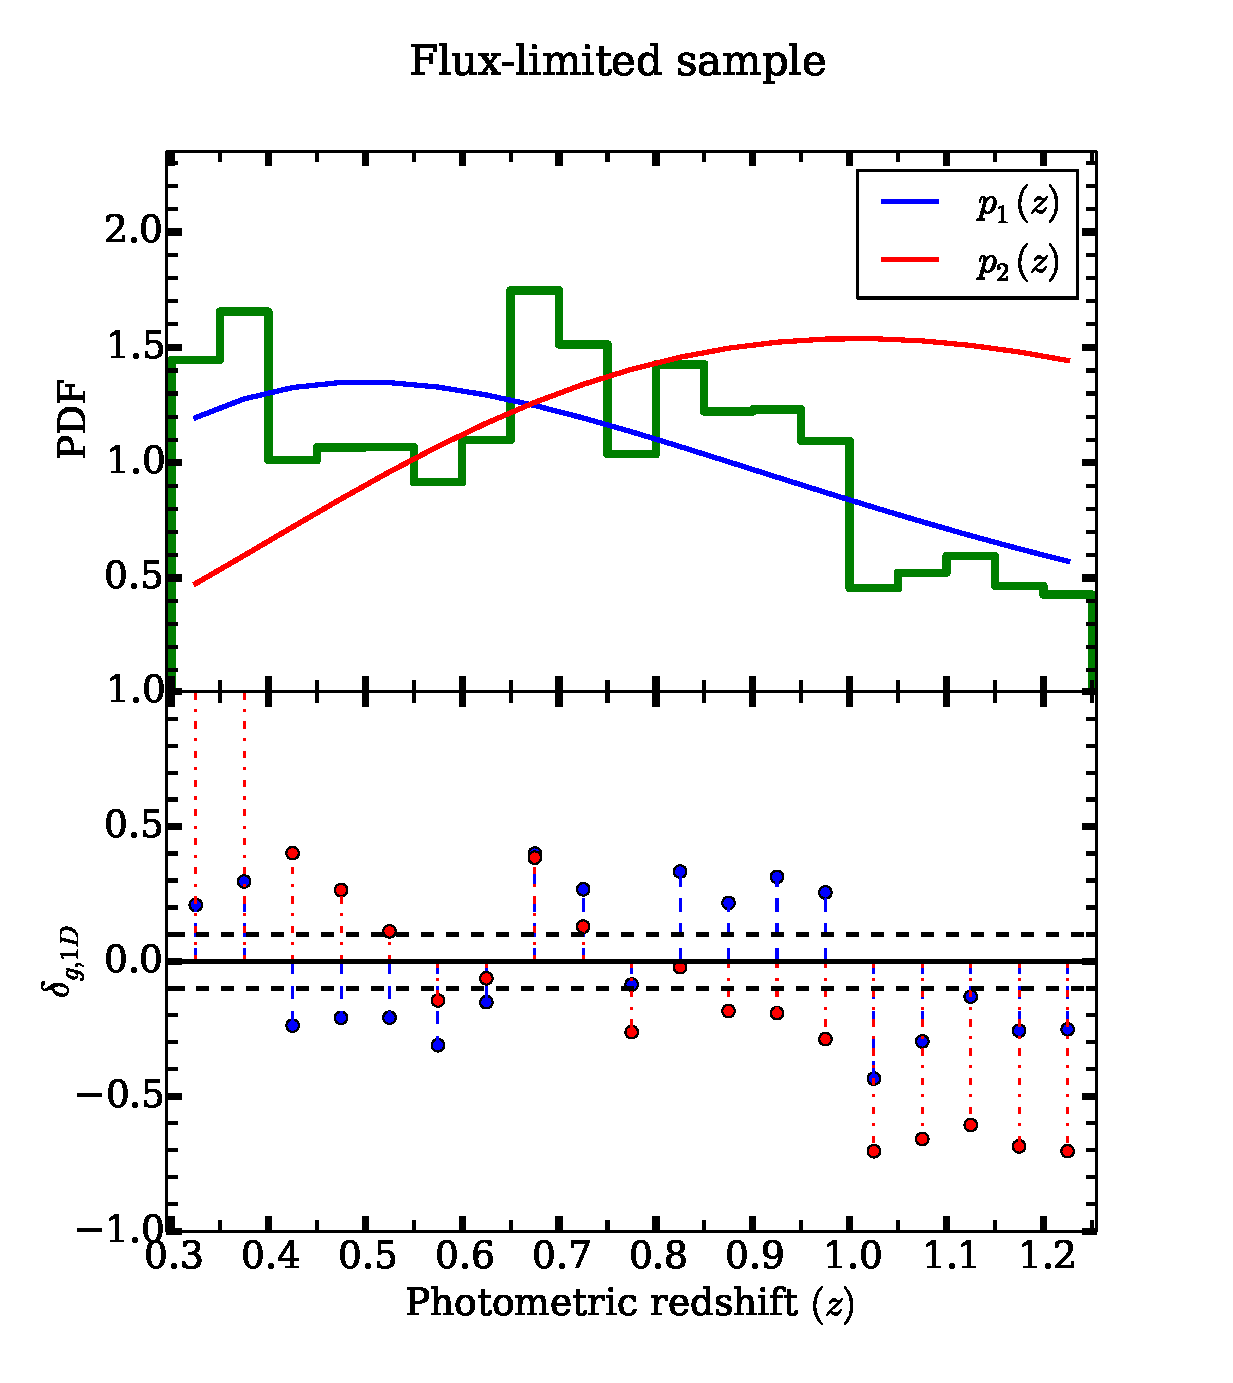
\includegraphics[width=\columnwidth]{redshift_fluxlimited}
  \label{fig:redshift_fluxlimited}
  \caption{}
\end{figure}

Overdensity in a redshift bin is defined as the ratio of the difference between the value given by the histogram and the value predicted by the model to the latter: $\delta=(N-N_{\text{mod}})/N_{\text{mod}}$. 
We leave a 10\% margin of safety i.e. iff $\delta$ from both the fits is greater than $0.1$, then we call that redshift bin as an
overdense region whereas if $\delta$ from both the fits is less than $-0.1$, then we call that as an underdense region. Redshift bins with $-0.1 < \delta < 0.1$ are neither too overdense
nor too underdense and we call them as `unclassified regions'  and discard them from our analysis.{\bf Fig 4 - overdensities vs redshift bins}.
\rachel{Let's not discard them.  We should just treat them as
  ``environmentally neutral.''  You do after all show them on your plots.}

% \begin{figure}
%  \centering
%  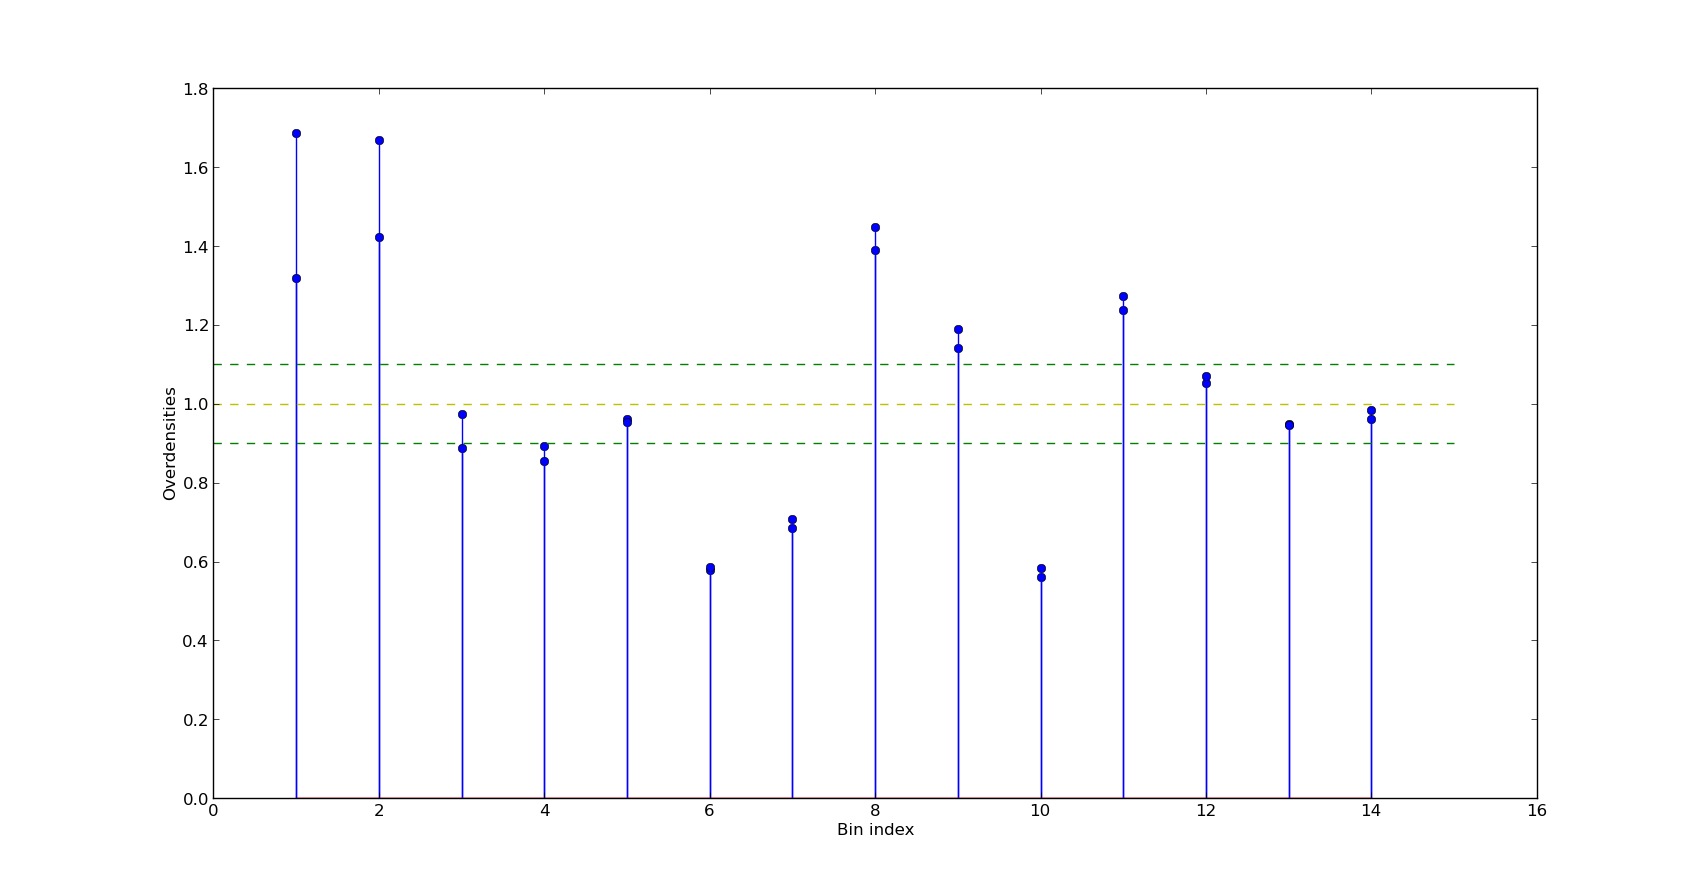
\includegraphics[width=\columnwidth]{fig4}
%  \label{fig:comoving_densities}
%  \caption{Differential comoving densities, integrated within a bin, are plotted. Red line refers to the average comoving density over the entire volume under consideration. 
%           The green lines correspond to the 0.9 and 1.1 times the overall average.}
% \end{figure}

We thus identify the regions $z=0.30-0.40, 0.65-0.75, 0.80-0.85$ as overdense, $z=0.55-0.65, 0.75-0.80$ as underdense and $z=0.40-0.55$ as unclassified.
The classification of overdensities and underdensities agrees with the work done by~\cite{Kovac_Density10k} on the zCOSMOS field using spectra and 3D density field reconstruction , except for the last two high redshift bins.
We believe that this disagreement is due to the errors in our photometric redshifts and the overdensity reported in $z=0.875-1$ slice
is observed by us in $z=0.80-0.85$ slice.

We see that the region between $0.85<z<1.0$ is neither overdense nor underdense according to our model and hence is not going to be considered for further analysis.

We use therefore relax our luminosity cut %to $-20.8$
so that the sample is volume-limited \emph{not} until $z=1$ but until $z=0.85$. 
We choose to impose the cut at $M_I=-20.8$, with 95.3\% completeness. This increases the sample size significantly, from 7,418 galaxies to 11,169.

\rachel{I think ``arbitrary'' is not the right word ot use in this
  paragraph.  It's obviously well-motivated in a general sense, and
  the question is whether it's robust or not.  Comparison with a more
  robust 3d method is what we use as validation to say that it's
  robust enough for our purposes.}
\arun{Done.}

\subsection{Volume limiting}
\label{sub:volumelimiting}
COSMOS is a flux-limited survey and is therefore affected by Malmquist bias, i.e. at higher redshifts, the brighter galaxies are preferentially observed.
Our analysis involves comparing galaxies in different redshift slices to find significant differences in morphology, if any, so with a flux-limited sample, we would be comparing only the bright galaxies at high redshifts with
bright and faint galaxies at low redshifts. For a fair comparison, we must restrict ourselves to bright galaxies at all redshifts and this is acheived by volume-limiting the sample.
%\rachel{Explain why you are doing this.  Before saying {\em how} you
%  generate a volume-limited sample, explain {\em why} you are
%  generating one.}
We generate, using the method below, a volume-limited sample that is complete upto $z=1$ by applying a cut on luminosity such that only galaxies instrinsically brighter than a certain threshold is considered. This threshold is set on $K$-corrected $i$-band magnitudes, denoted as $M_I$.
Since the parent sample contains fainter galaxies, upto F814W=25.2, we compare the distribution of the F814W=23.5 sample with the samples containing fainter galaxies for high redshift bins, to see where the sample is no longer complete.
\begin{figure}
 \centering
 a) 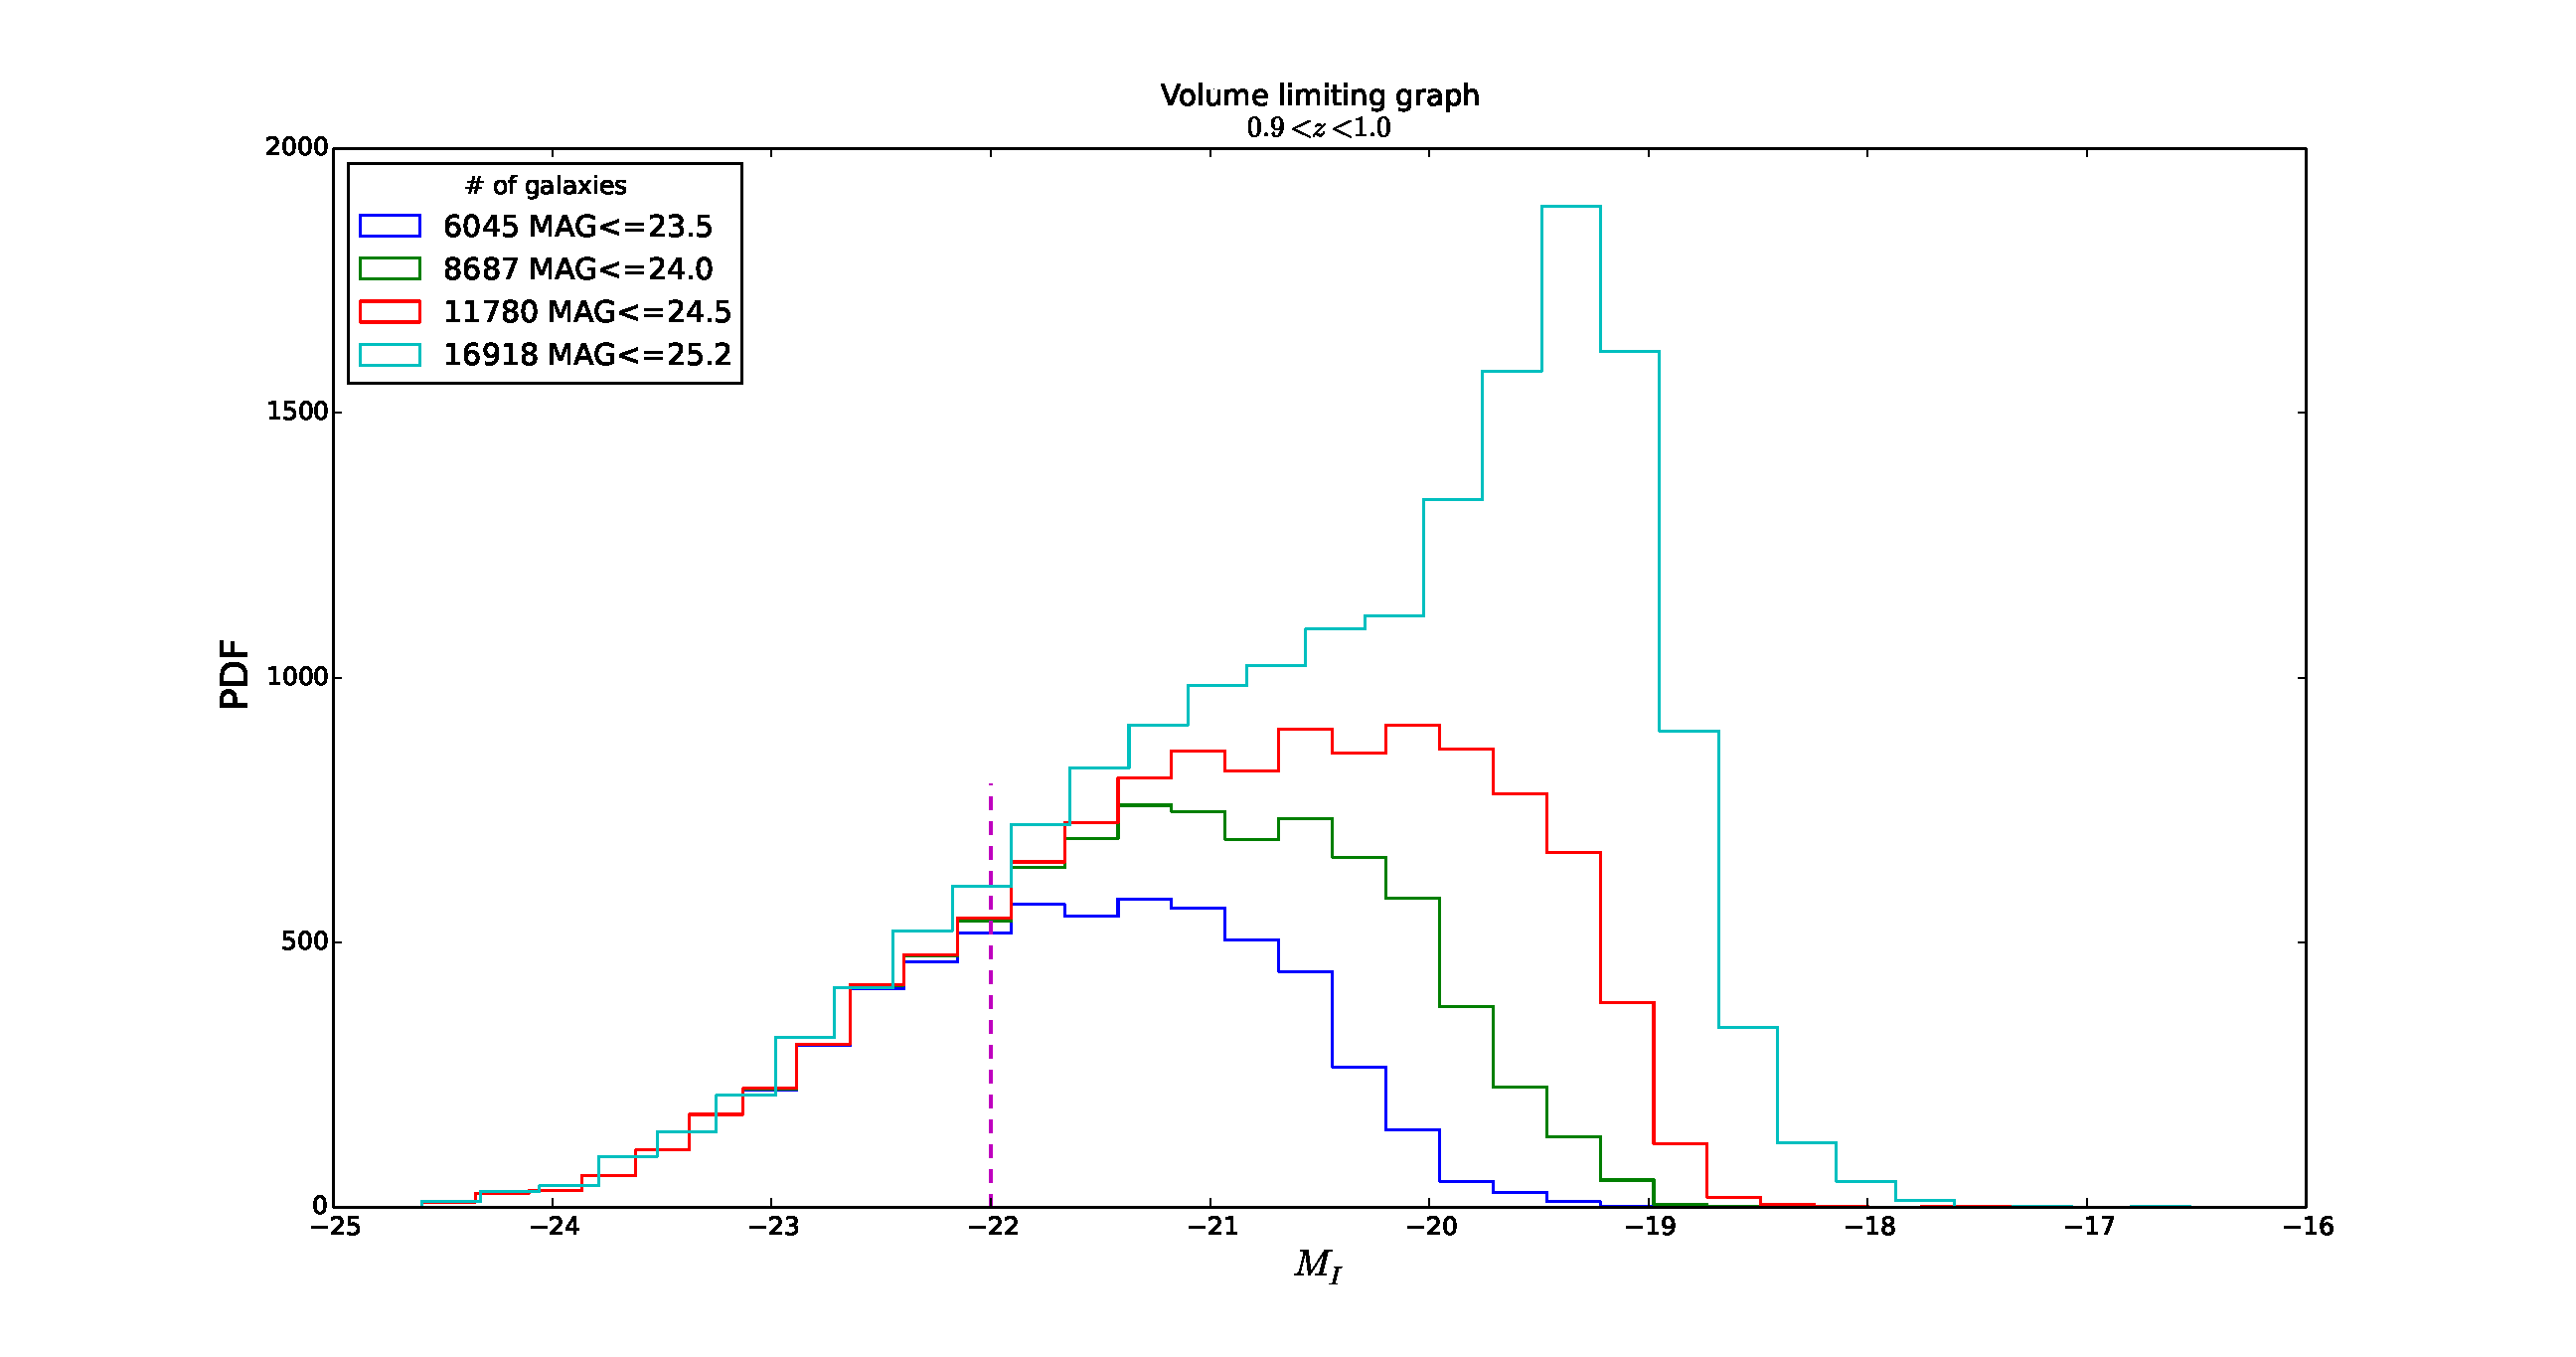
\includegraphics[width=\columnwidth]{volume_limiting_pdf}
 b) 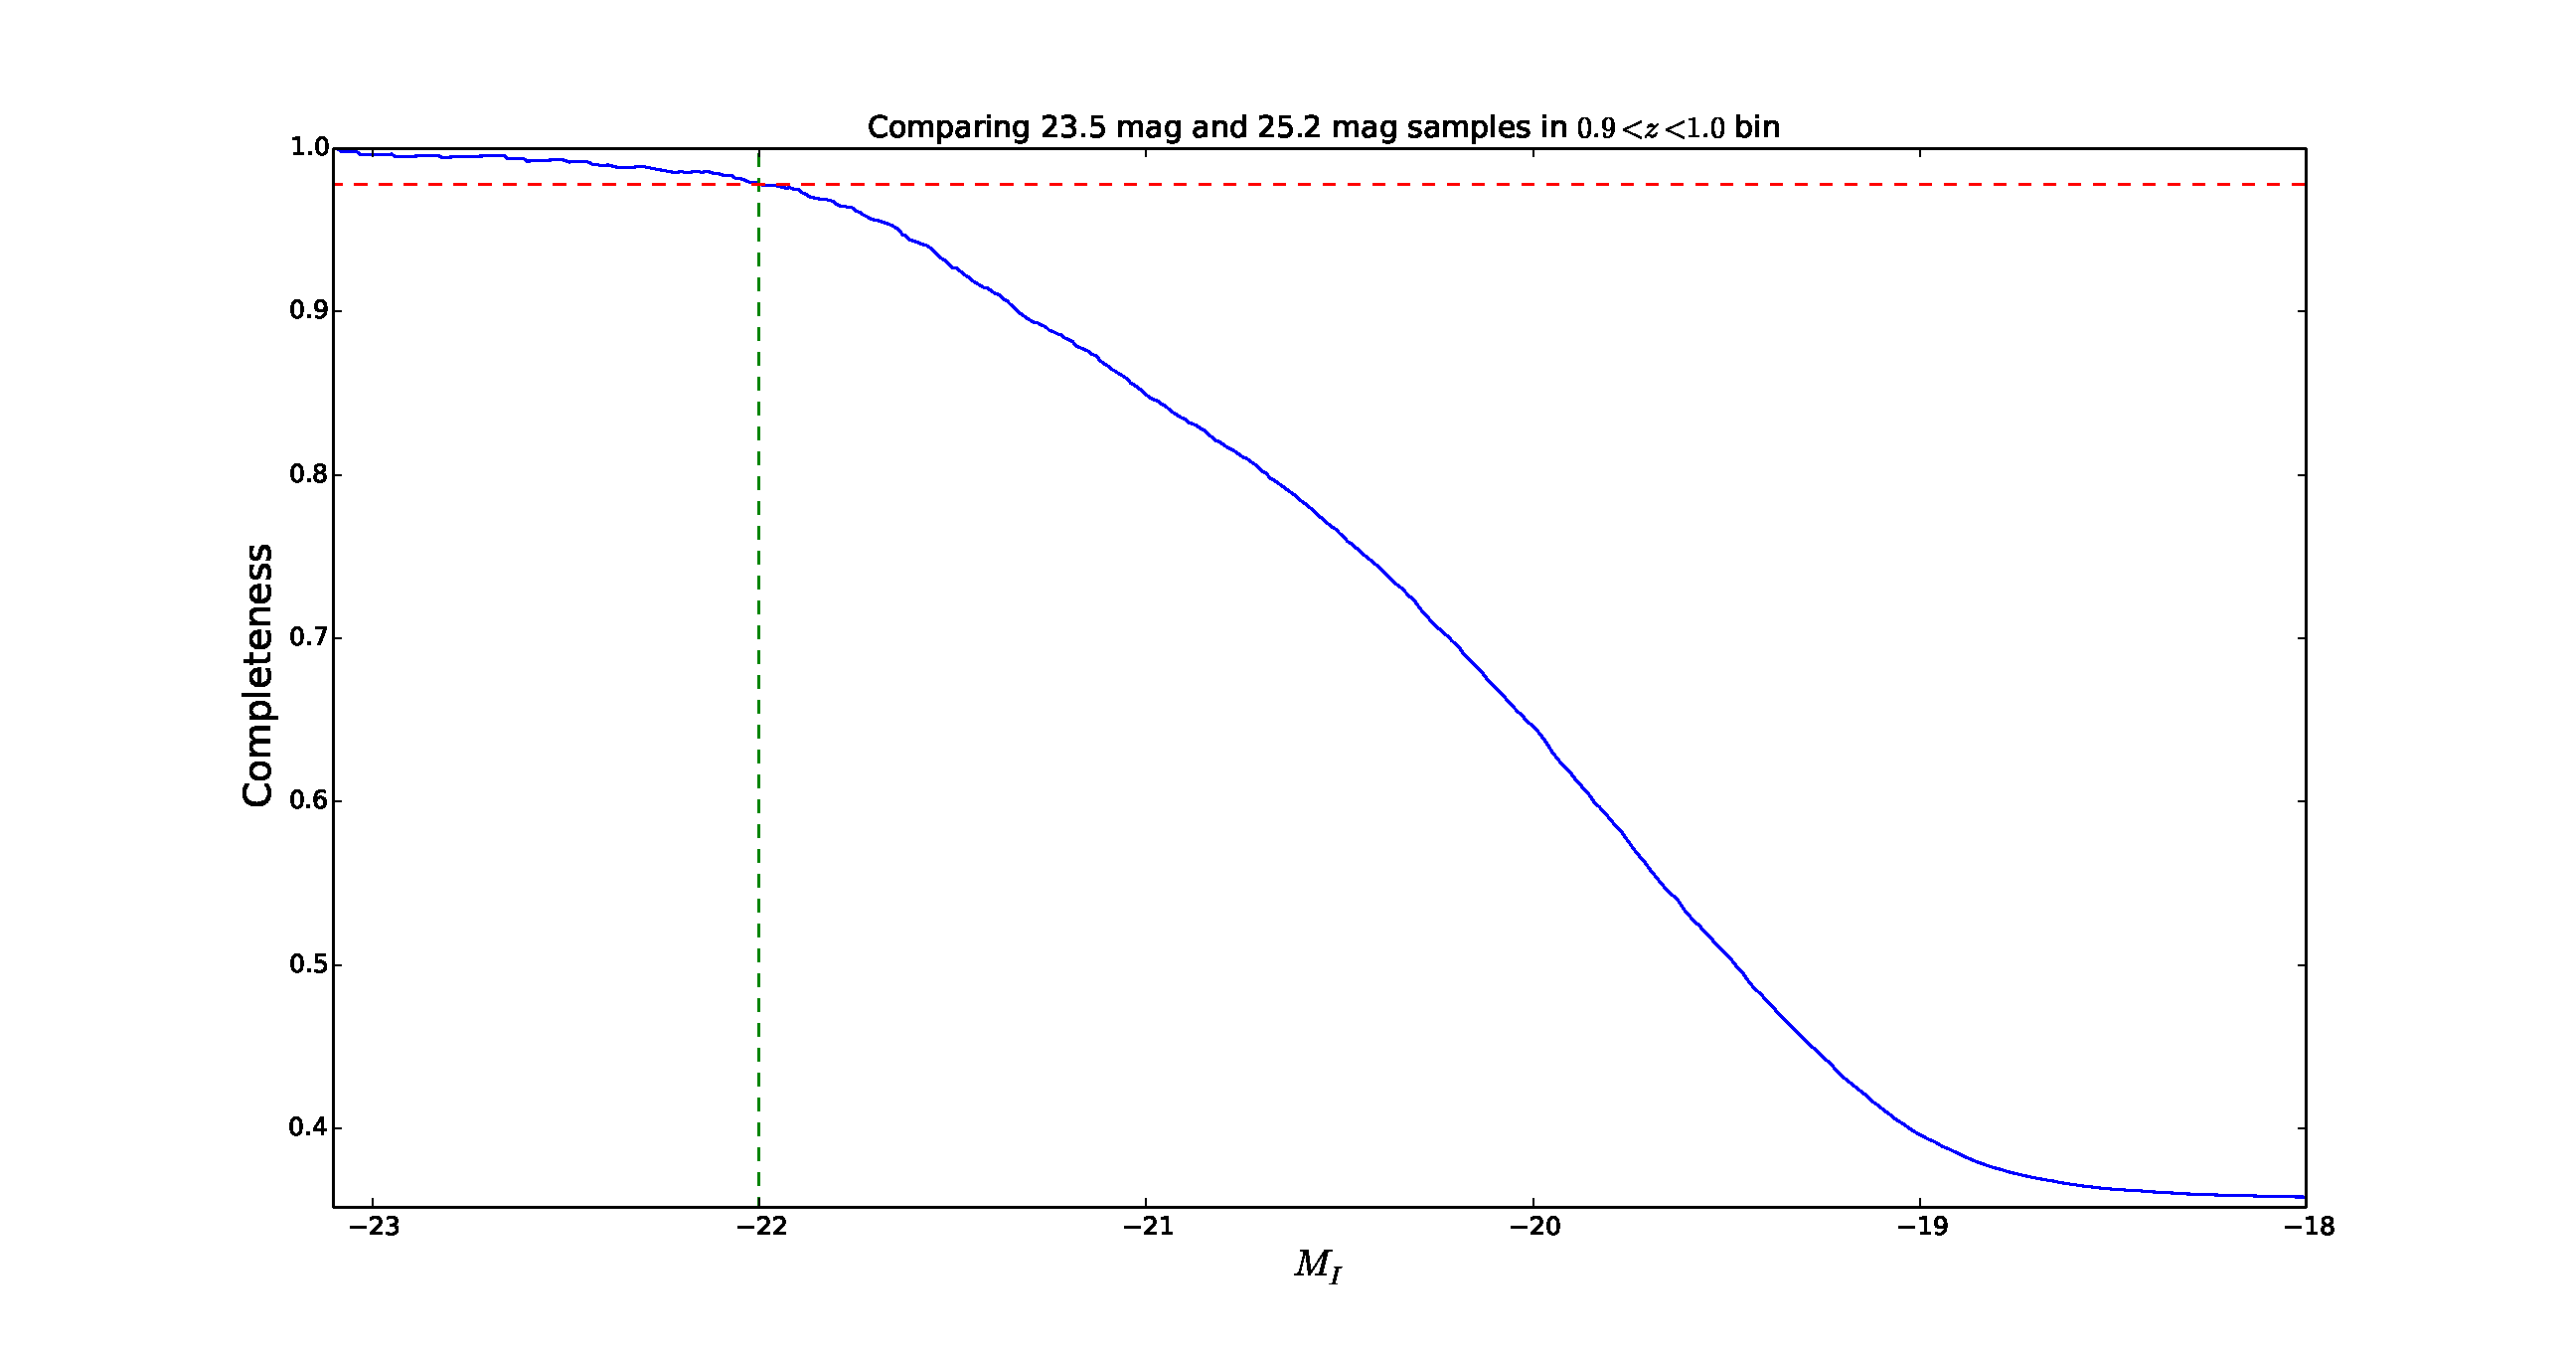
\includegraphics[width=\columnwidth]{volume_limiting_cdf}
 \label{fig:volume_limiting_dist}
 \caption{ ... }
\end{figure}

At $M_I\sim-22.0$, we see the sample is beginning to be biased in the $0.9<z<1.0$ bin due to the flux limit. We obtain 97.84\% completeness in this bin for $M_I$, where completeness is defined as the ratio between the number of galaxies in F814W$\le$23.5 and in F814W$\le$25.2 samples.
Thus the sample $z\le1$ and $M_I<-22$ is at least 97.84\% complete. Fig.~\ref{fig:2Dhist} shows that at $M_I<-22$, we are not affected by flux limit yet. 

However, previous studies {\bf cite} have shown that absolute luminosities evolve with redshift. Thus, we must also let the luminosity cut evolve with the redshift. 
There has been no published literature on the LF for the $I$-band, particularly for the COSMOS survey.
We used the published result~\citep{Faber2007} for the `rate' of evolution of B-band magnitudes for DEEP2 and COMBO-17 surveys, which is $ \Delta M_B^* \sim -1.23$ mag per unit redshift, for both blue and red galaxies combined together.
Typically, estimates of evolution in K-band are lesser than the estimates of evolution in B and V bands.
Assuming that the evolution is a smooth function of the wavelength, the evolution in I-band is expected to be lesser than that of the B-band. 
Thus, by considering no evolution and an upper bound on the evolution, we can interpolate what the results would be like for the true $I$-band evolution.

%In our analysis, we imposed the cut on luminosity for all redshift bins while many studies have shown that the characteristic luminosity of galaxies evolve with redshift. 
% The work that is at least close to what we expect is that of
%~\cite{Faber2007}, who have studied the evolution of Schechter parameters in the B-band of DEEP2 and COMBO-17 surveys. We consider their reported value of $ \Delta M_B^* \sim -1.23$ per unit redshift, for both blue and red galaxies combined together.
%Although it is the $I$-band that is of relevance to us, we expect the evolution in B-band to be an upper bound on the evolution in I-band. 


%Alternatively, we can impose cuts on stellar mass of the galaxies instead of imposing on the luminosity. 
%If we restrict to galaxies with masses $M$ such that $\log(M/M_\odot) \ge 10.15$, then we have at least {\bf 95.0\% } completeness.
Alternatively, one could get around the problem of considering redshift evolution by imposing cuts on stellar mass instead of absolute luminosity in a particular band. In Fig.~\ref{fig:smf}, we show the stellar mass function (SMF) of our sample for various F814W flux limit.
\cite{Tomczak_SMF} report the SMFs for the ZFOURGE survey, which includes COSMOS. They considered for this work, a single stellar population following a Chabrier{\bf cite} IMF. 
We plot their SMF for \emph{all} in ~\ref{fig:smf} for reference. Their SMF is higher than ours since they reach $K_s$-band $5\sigma$ depth of 24.9 {\bf What exactly does this mean?}
As in the case of $M_I$ s, we compare the stellar mass in the F814W$\le$23.5 sample with that of the F814W$\le$25.2 sample. 
The sample $\log(M/M_\odot) > 10.15$ is about 95\% complete in the redshift bin $\left[ 0.75 - 0.85\right]$ and has 10,341 galaxies in total.

\begin{figure*}
 \centering
 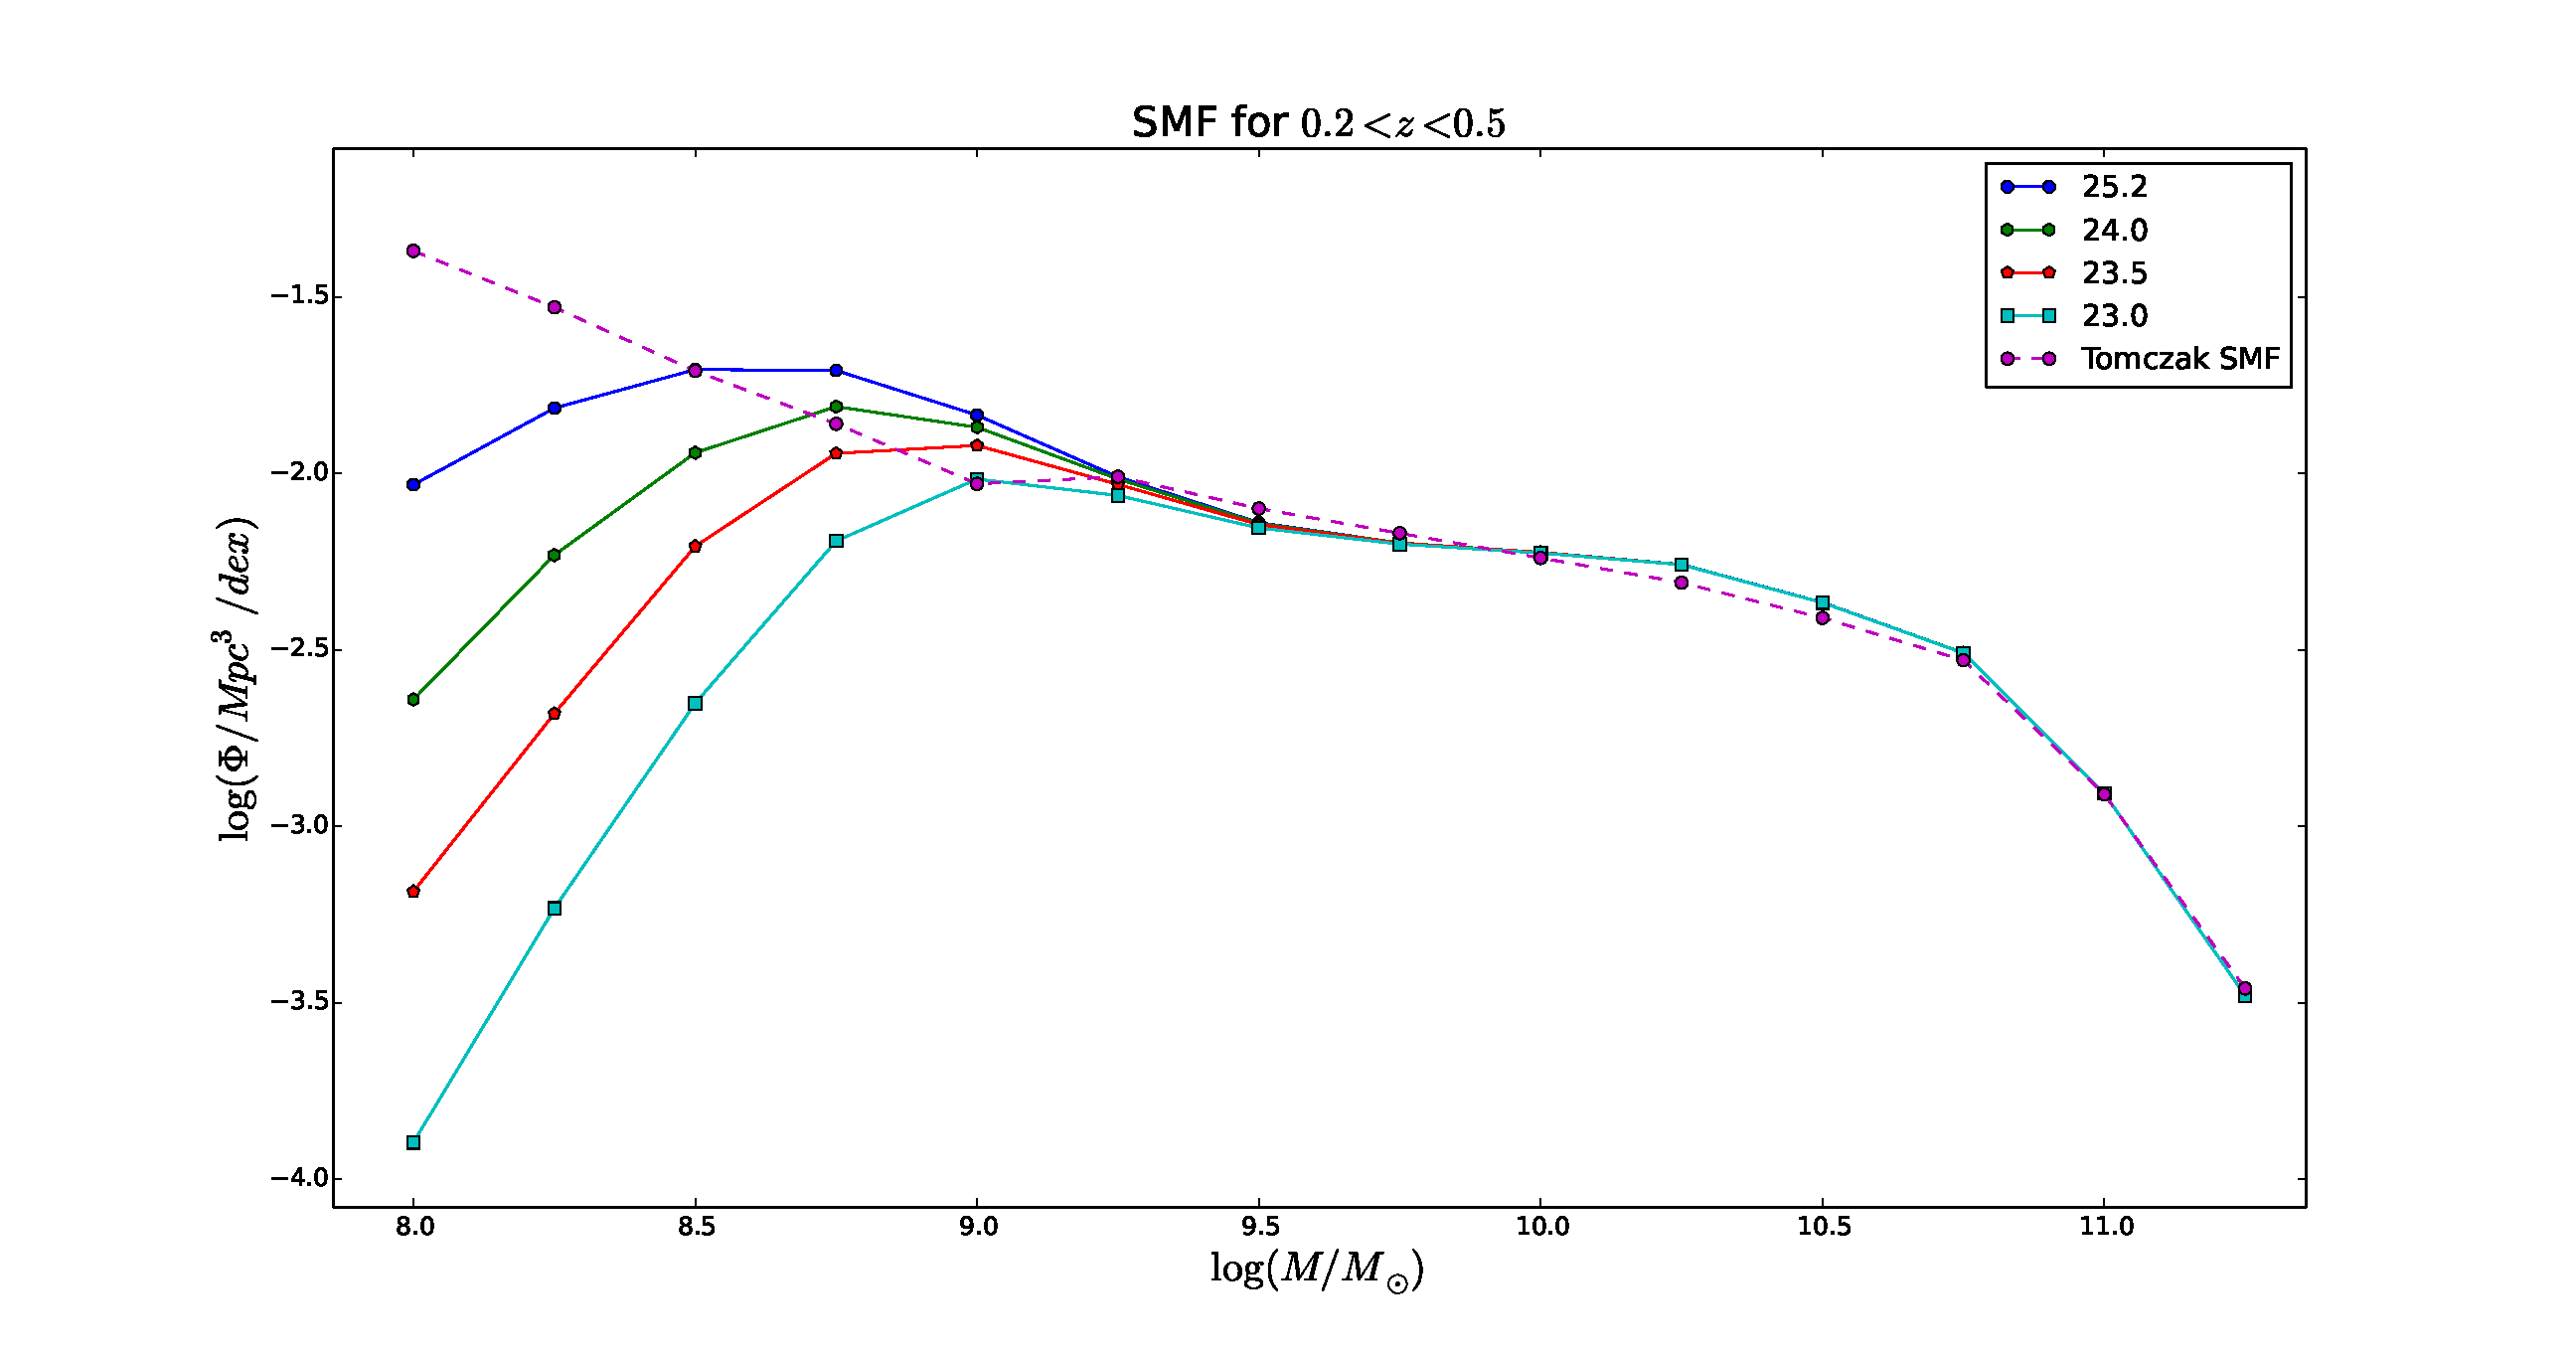
\includegraphics[width=0.66\columnwidth]{SMF1} \
 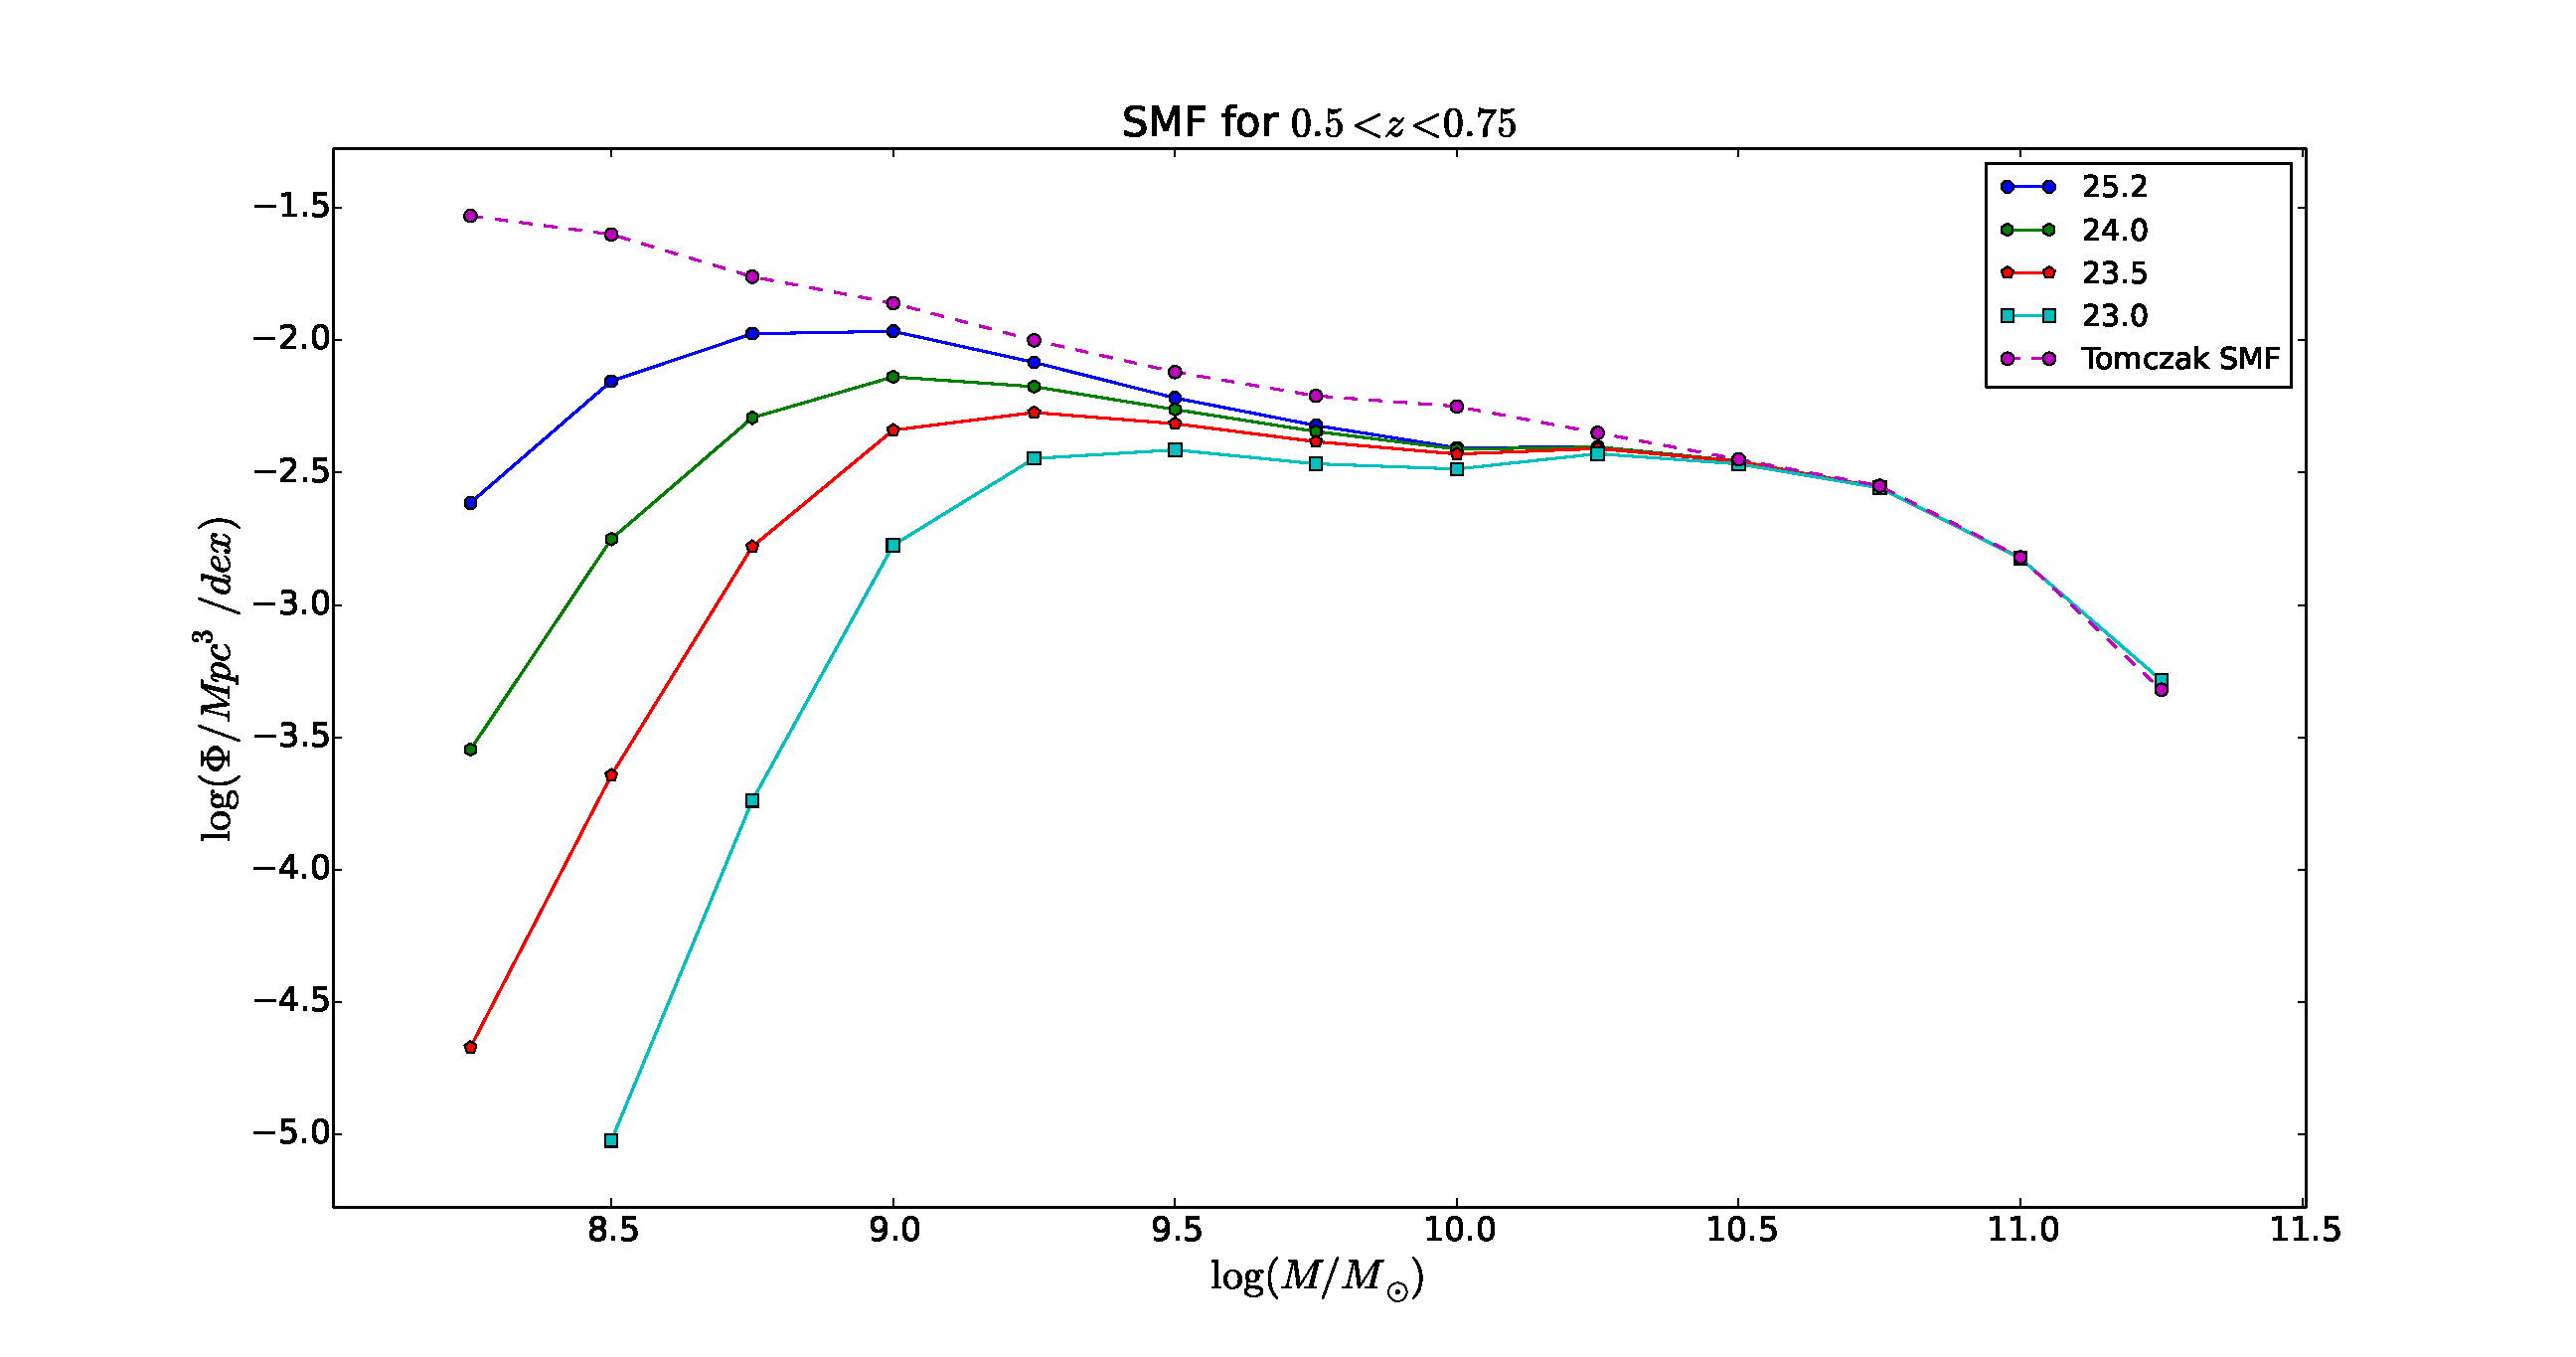
\includegraphics[width=0.66\columnwidth]{SMF2} \
 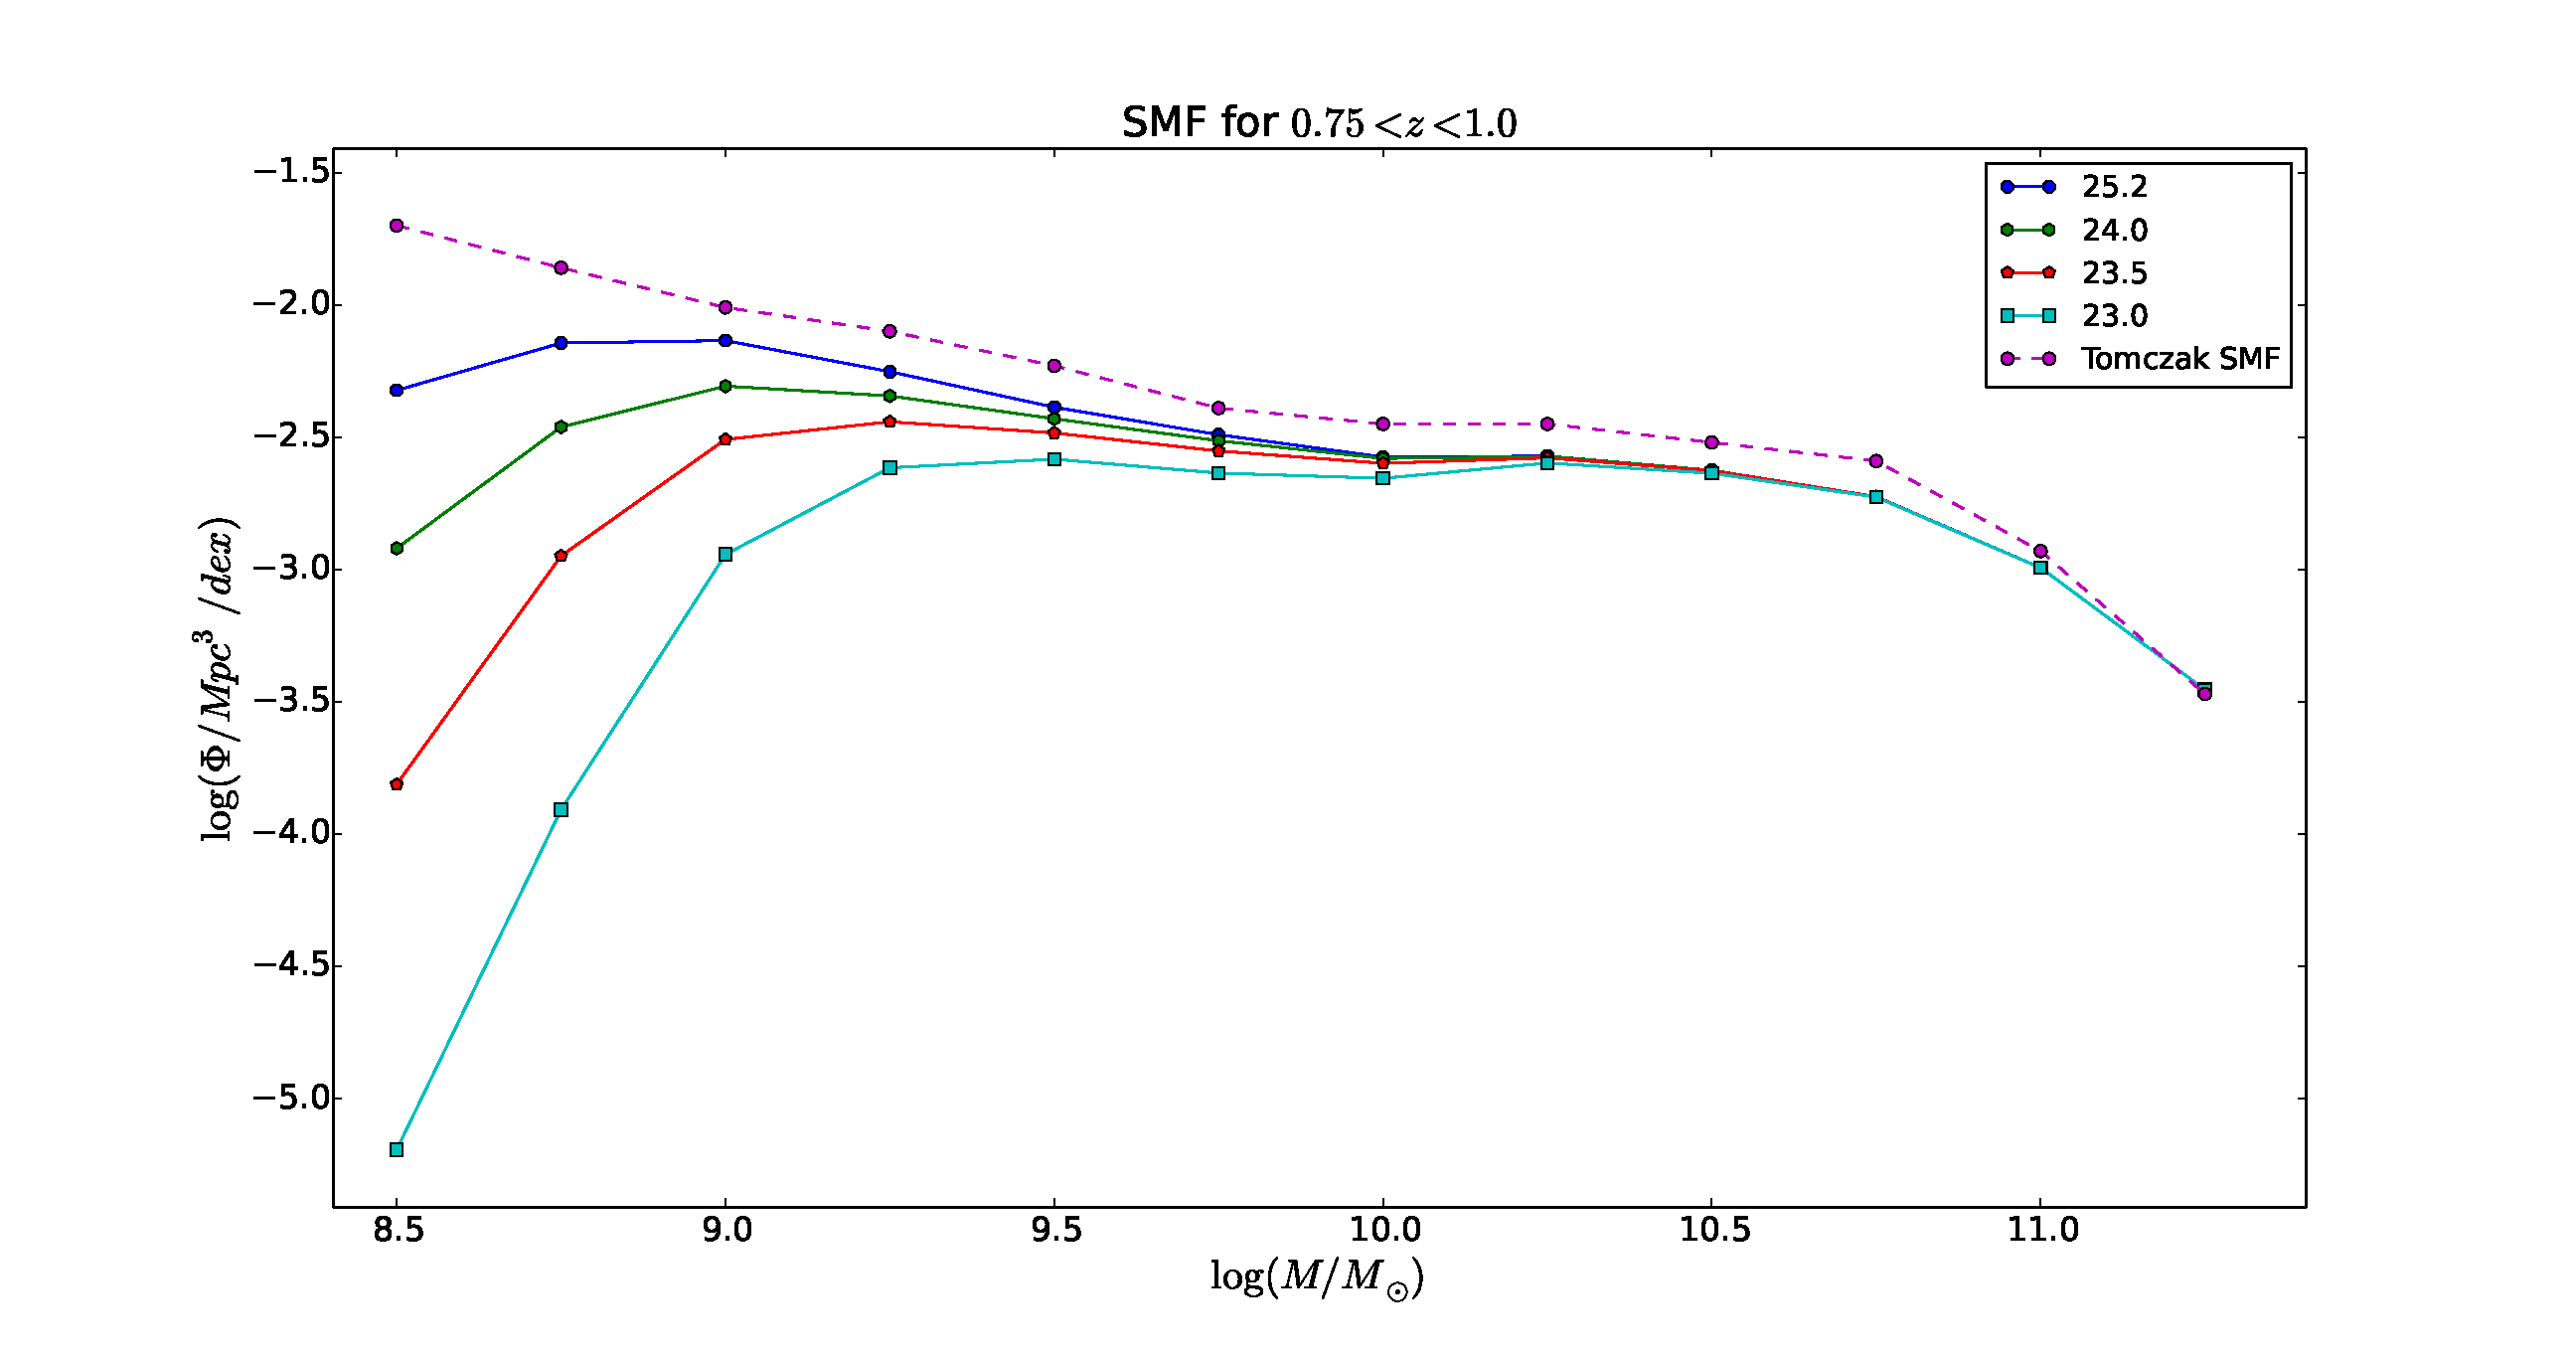
\includegraphics[width=0.66\columnwidth]{SMF3}
 \caption{SMF plots}
 \label{fig:smf}
\end{figure*}

There is a minor pitfall with this method. We analyse only those galaxies for which postage stamp images exist.
Postage stamps may not exist either because the image occurs near the edge of the CCD chips or because the image is too large to fit in a bounding box. \arun{Rachel, please correct my terminology here.}
While the former is purely random and doesn't introduce bias, the latter is not. Typically galaxies that are nearby and intrinsically very bright do not have postage stamps associated with them and this effect is dominant at lower redshifts. 
Thus, we use the full F814W$\le$23.5 sample, irrespective of the existence of postage stamps, and believe that our conclusions are not affected by this bias.

Not surprisingly, we see the overdense and underdense regions obtained by the above method have local average number density higher than the global average number density after volume limiting. %Refer to Figure~\ref{fig:comoving_densities}.
And the environmentally neutral regions fall below or at least lie close to the 10\% margin.
%Refitting the model to our new sample is consistent with the previous assignment of overdensities.

\begin{figure}
 \centering
  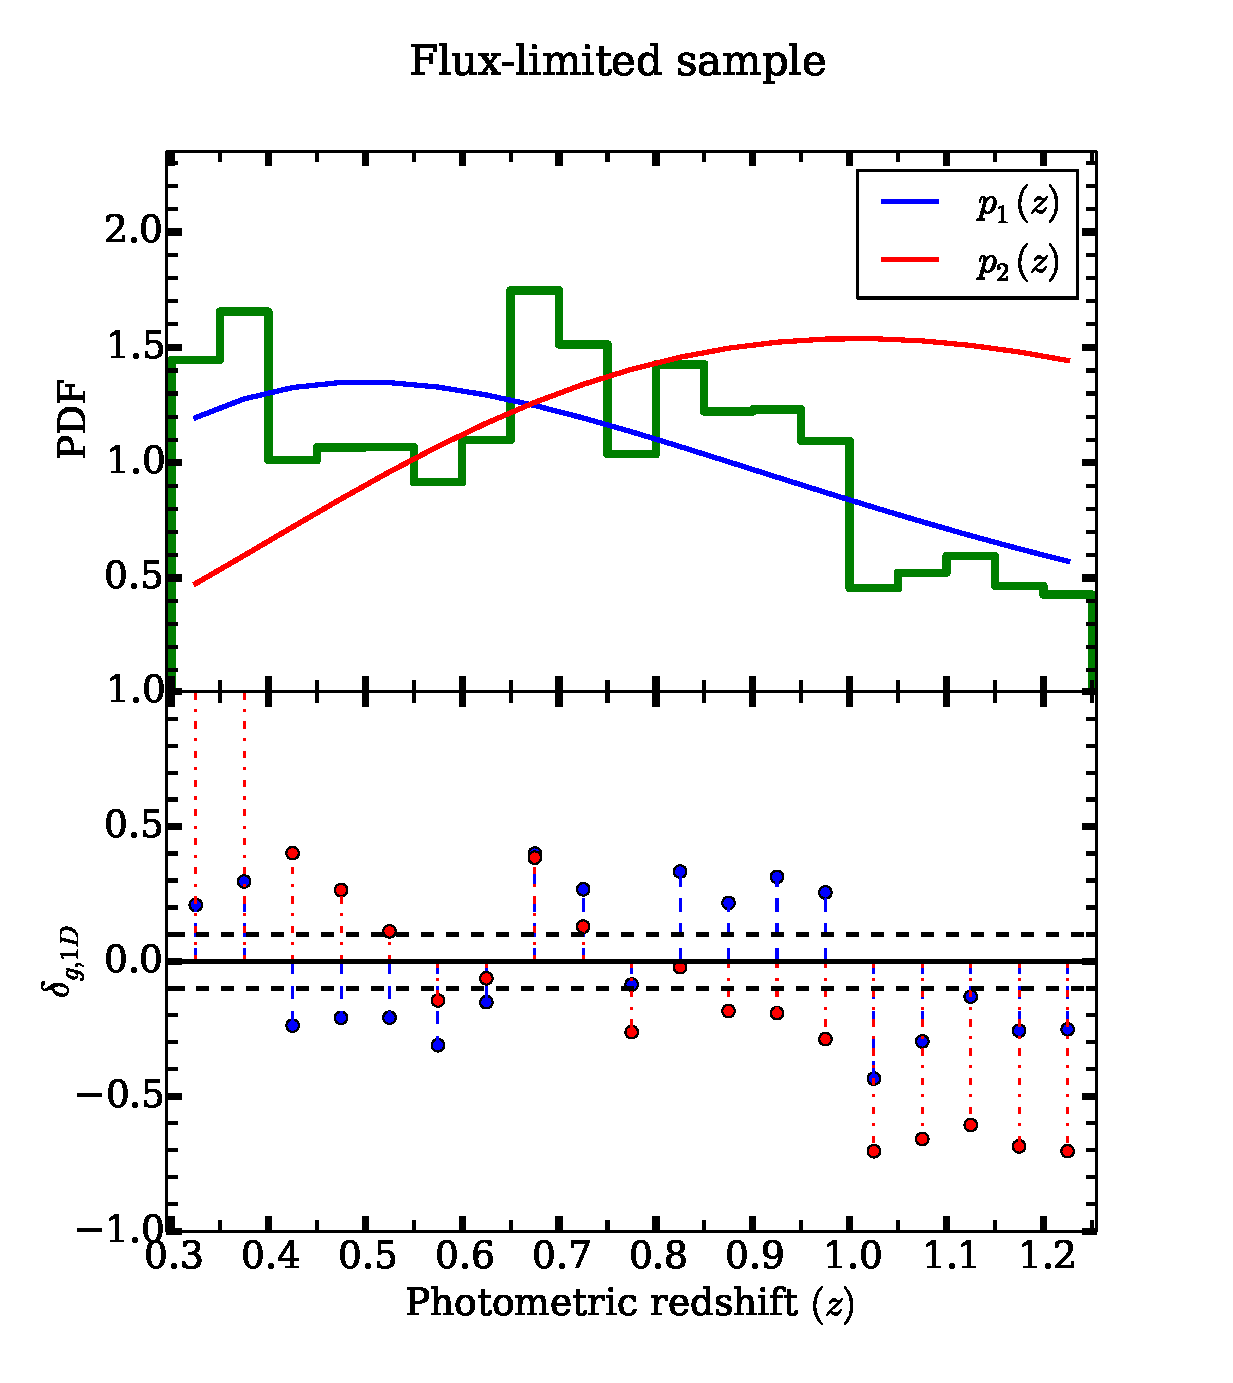
\includegraphics[width=\columnwidth]{redshift_fluxlimited}
  \label{fig:redshift_fluxlimited}
  \caption{}
\end{figure}

% \begin{figure}
%  \centering
%  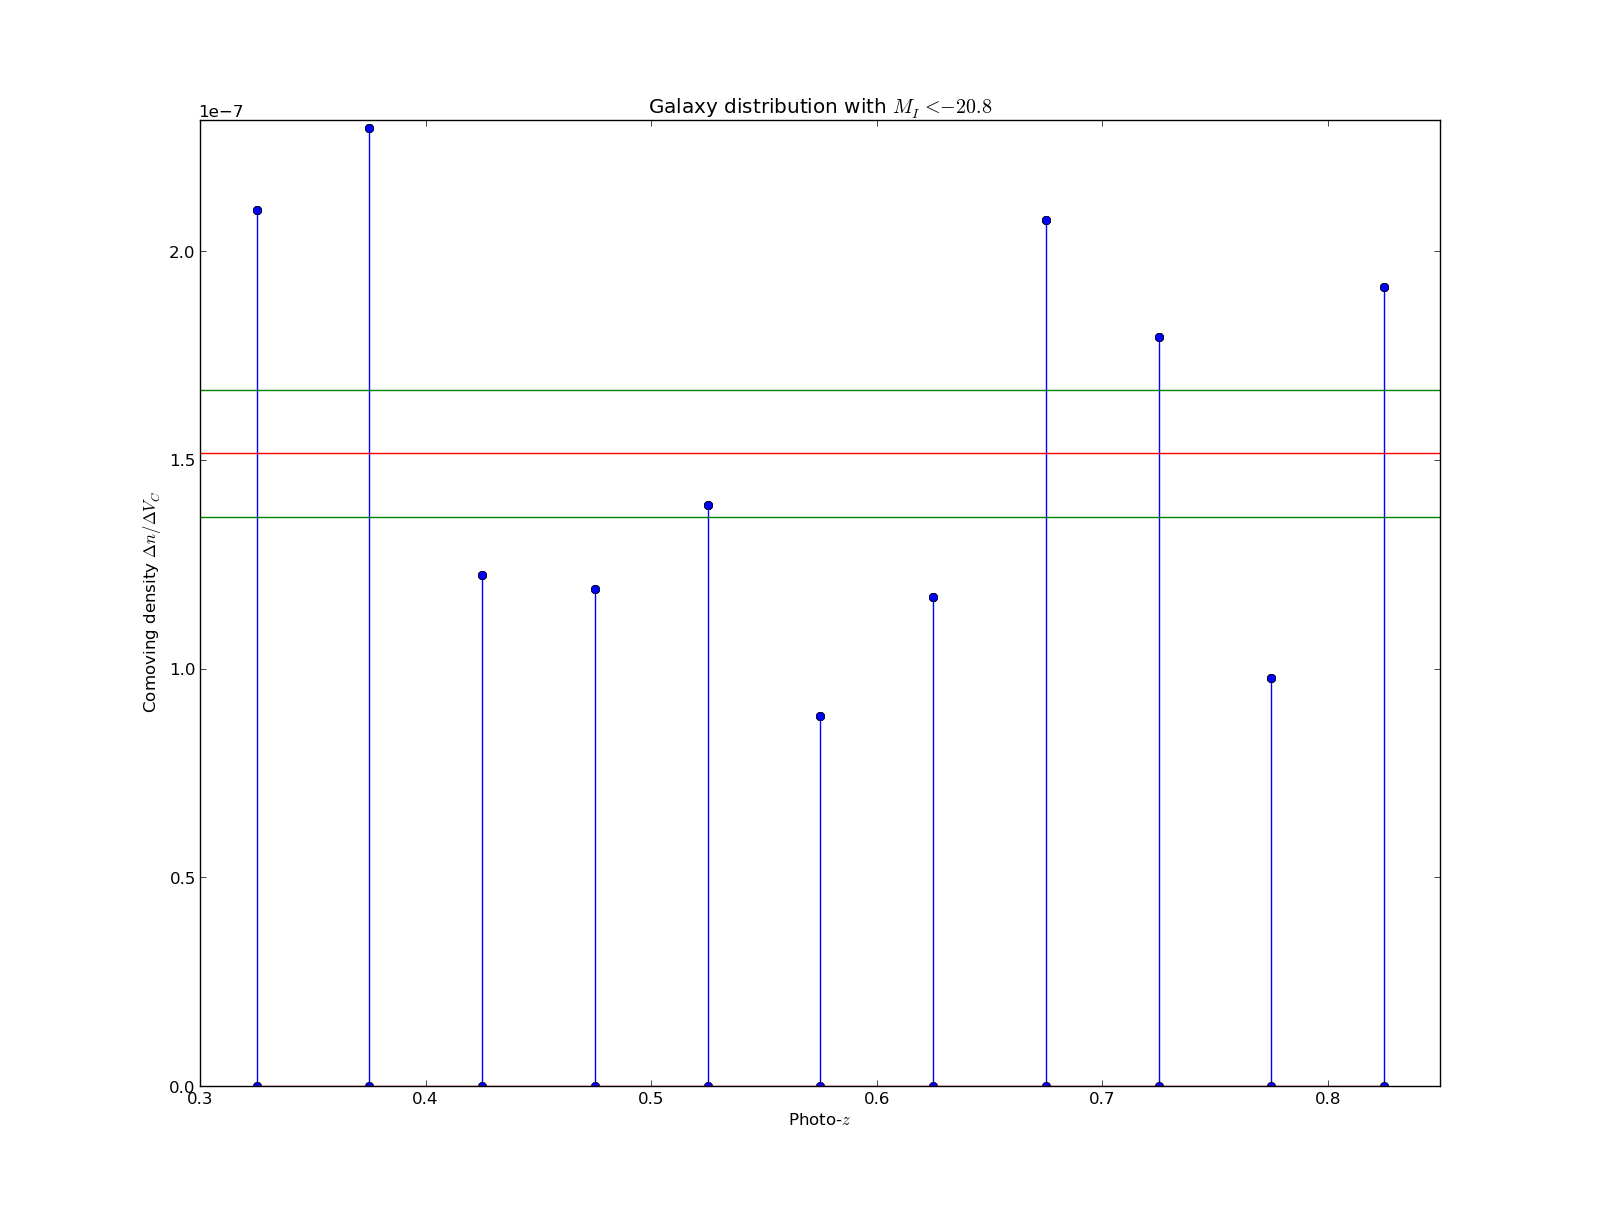
\includegraphics[width=\columnwidth]{../plots_20140219/comoving_densities(2b).png}
%  \label{fig:comoving_densities}
%  \caption{In computing comoving densities, we have chosen the following values for the $\Lambda$CDM parameters: $\Omega_m = 0.3, \Omega_\Lambda = 0.7 \text{ and } \Omega_k = 0$ with the Hubble parameter $h = 0.72$.}
% \end{figure}

\begin{figure}
  \centering
   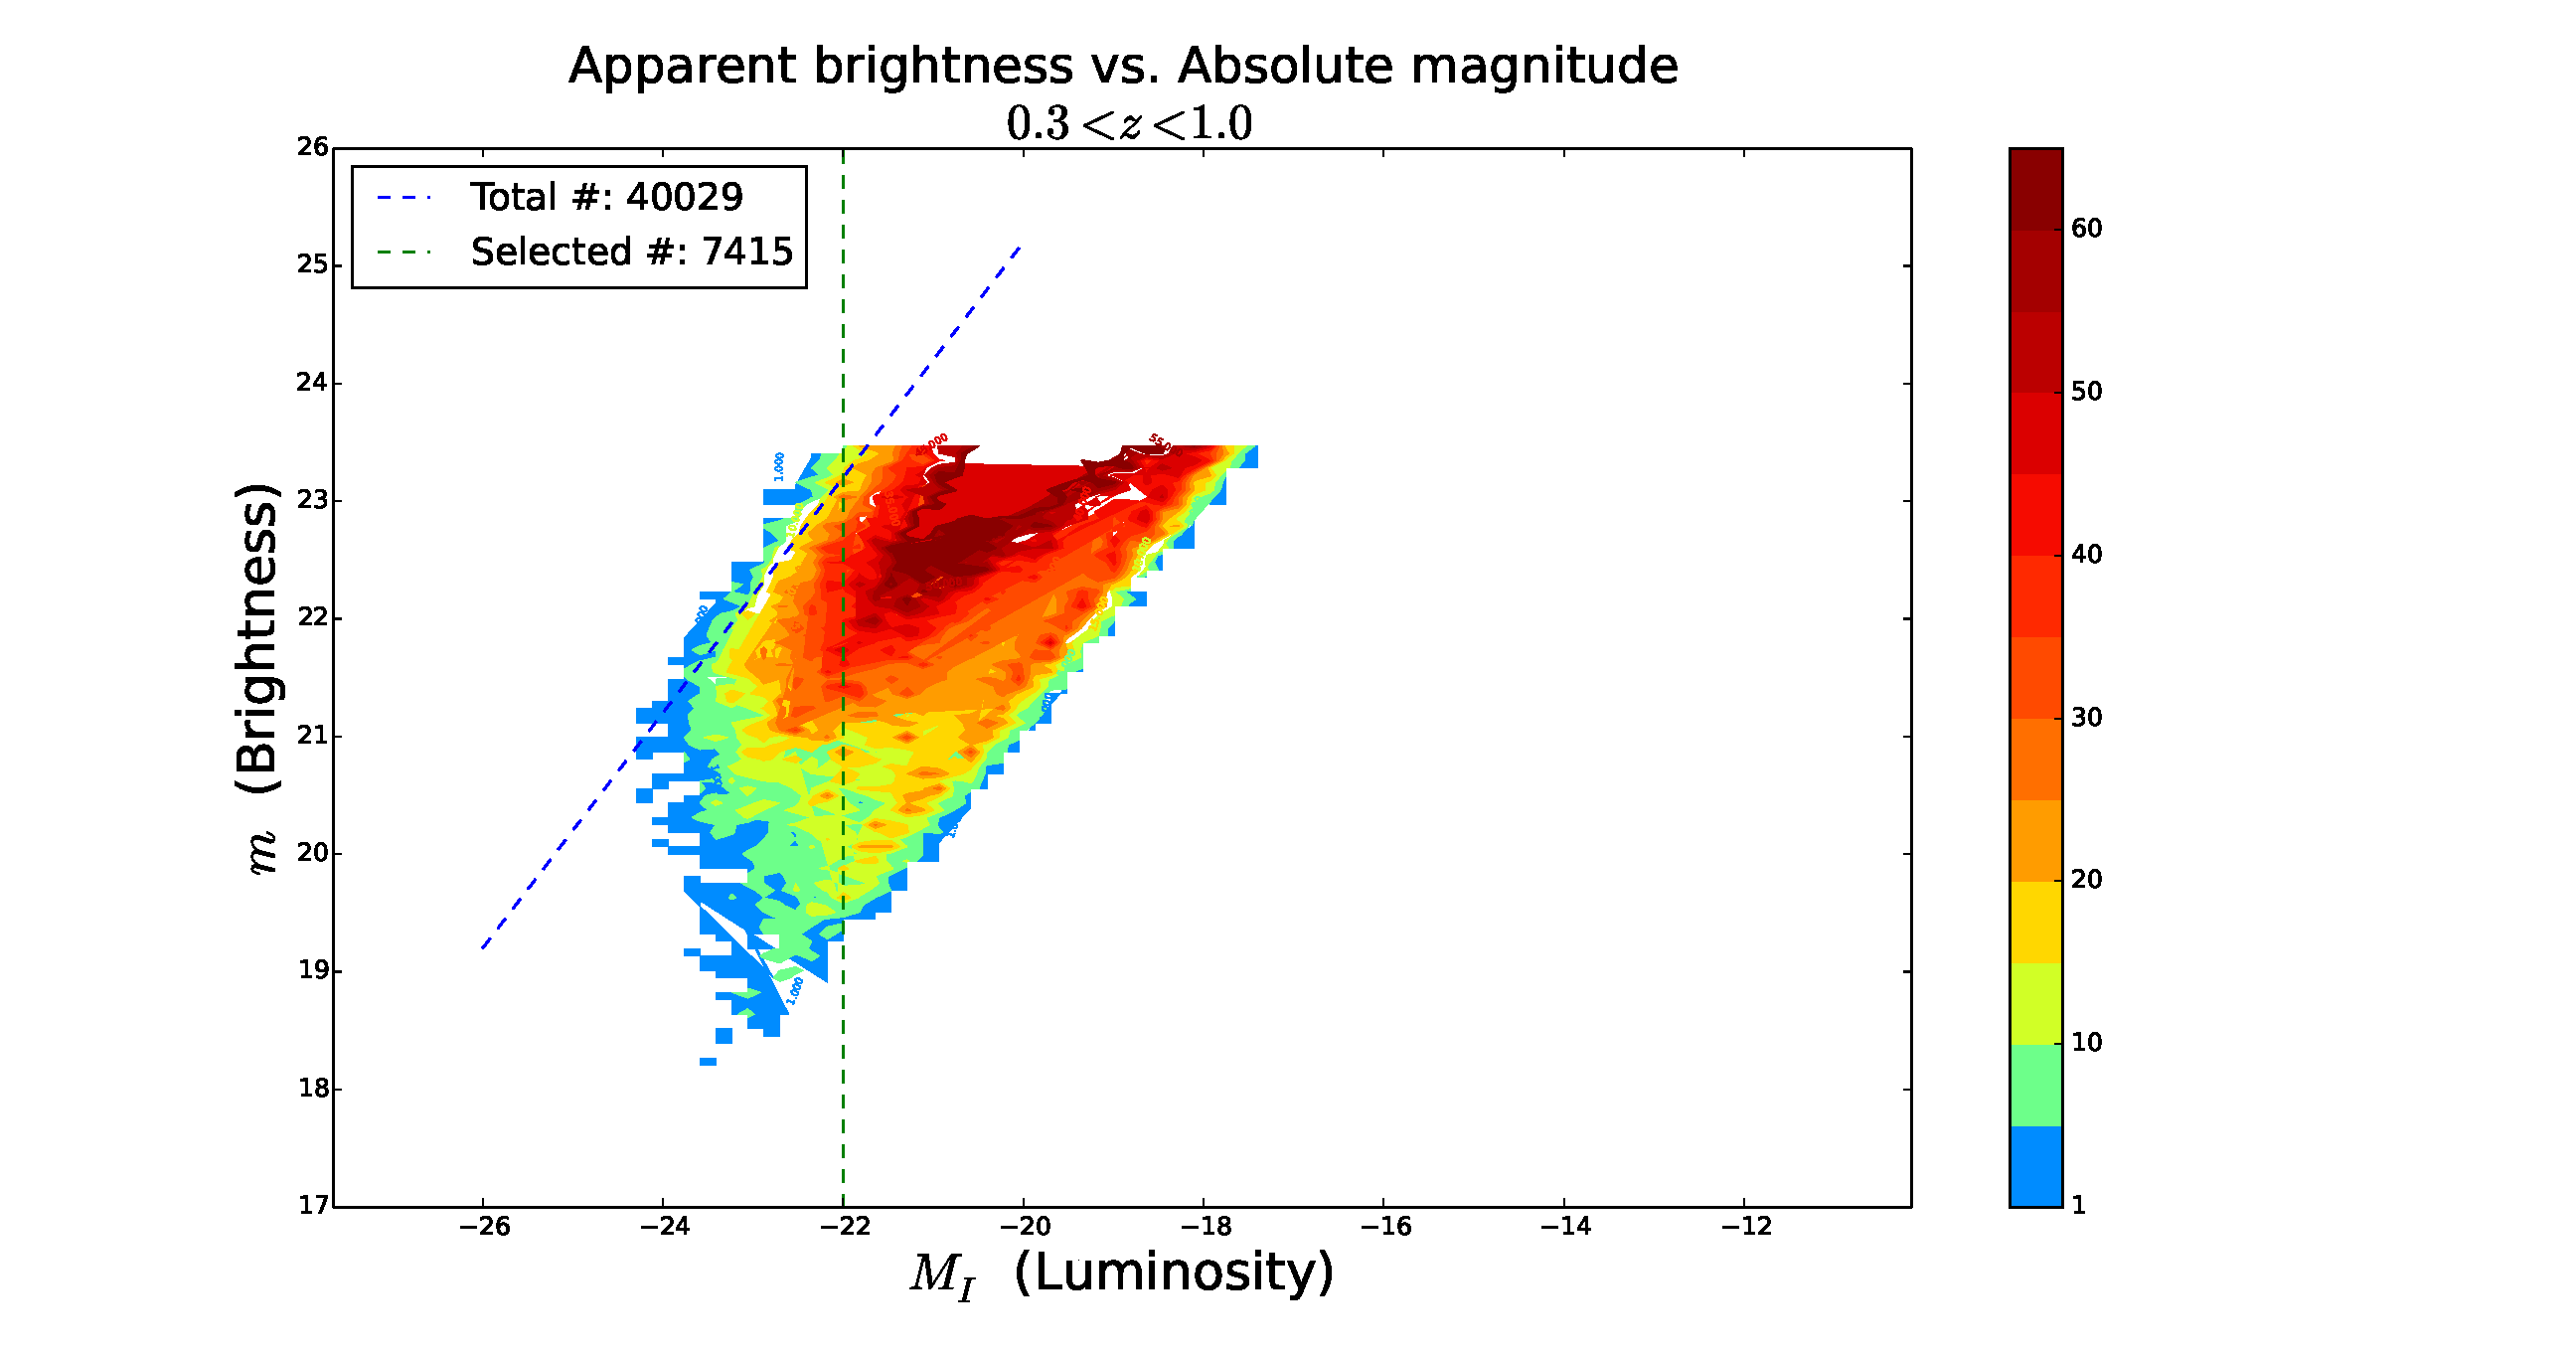
\includegraphics[width=\columnwidth]{hist2d_mag_mi}
   \caption{2-D histogram of galaxies in apparent magnitude ($m$) and absolute magnitude ($M_I$) space.}
   \label{fig:2Dhist}
 \end{figure}
  

\begin{tabular}{c|c|c|}
 \hline
 Redshift & \# of galaxies & Environment \\
 \hline
 0.30-0.35 & 726 & Overdense \\
 0.35-0.40 & 1000 & Overdense \\
 0.55-0.60 & 727 & Underdense \\
 0.60-0.65 & 1070 & Underdense \\
 0.65-0.70 & 2089 & Overdense \\
 0.70-0.75 & 1970 & Overdense \\
 0.75-0.80 & 1159 & Underdense \\
 0.80-0.85 & 2428 & Overdense \\
 \hline
\end{tabular}

In the following section, we will compare and analyze the distribution of properties of the galaxies residing in the overdense regions.

\emph{Talk more about environments - Nature and nurture?}

%\section{Implications/Comparisons}
%\section{Results}
\subsection{Finding fit parameters}
\label{sub:axisratio}
{\bf Should explain in brief Claire's work.} \\
If galaxies have elliptical isophotes, its shape and size could be defined by the axis ratio and the area enclosed by a boundary isophote. However, in real galaxy images,
the boundary may not be well defined and the shape may not be well approximated by an ellipse. Given the surface brightness (intensity) $I(\vec{\theta})$ of a galaxy image at every angular position $\vec{\theta}$,
we can define the tensor of second brightness moments as
\begin{equation}
 Q_{ij} = \frac{\int\rmd^2\theta q_I (\theta_i - \overline{\theta_i})(\theta_j - \overline{\theta_j})}{\int\rmd^2\theta q_I},
\end{equation}
where $q_I$ is a suitable chosen kernel and $\overline{\vec{\theta}}$ is the average angular coordinate, weighted by the same kernel function and $i,j\in\lbrace 1,2 \rbrace$ are the componenets of $\vec{\theta}$.
It is common to find in literature two kinds of \emph{complex }ellipticities that quantify the shape of the galaxies - $\chi$ and $\epsilon$ defined as
\begin{align}
 \chi &= \frac{Q_{11}-Q_{12}+2iQ_{12}}{Q_{11}+Q_{22}} \\ \epsilon &= \frac{Q_{11}-Q_{22}+2iQ_{12}}{Q_{11}+Q_{22}+2(Q_{11}Q_{22}-Q_{12})^{1/2}}
\end{align}
If the image has elliptical isophotes with axis ratio $q$, then 
\begin{equation}
 |\chi| = \frac{1-q^2}{1+q^2}, \;\;\; |\epsilon| = \frac{1-q}{1+q}. 
\end{equation}


Conversely, one could compute $\chi$ or $\epsilon$ for a galaxy, and obtain an effective, azimuthally averaged {\bf(?)} axis-ratio $q$. 
\rachel{No, that isn't possible because of the PSF.  One would have to
  use a PSF correction scheme.  Recommend removing much of the above discussion.}
\arun{Should I remove these even if we plan to use the ellipticities from the second moments?}  
However, our method of finding the value of $q$ is little more complicated. Briefly, we fit
two models to each image:
\begin{enumerate}
 \item a \sersic profile given by the expression 
       \begin{equation} 
    S = \Sigma_{1/2}\exp{\left( -k(R/R_{\text{eff}})^{1/n} -1 \right)},
       \end{equation}
       \item two \sersic component fits: de Vaucoulers bulge $(n=4)$ + exponential disc profile $(n=1)$,
\end{enumerate}
where \begin{align*} R^2 = & ((x-x_0)\cos\Phi+(y-y_0)\sin\Phi)^2  \\ & + ((y-y_0)\cos\Phi-(x-x_0)\sin\Phi)^2/q^2, \end{align*}
$R_{\text{eff}}$ is the half-light radius of the profile, $\Sigma_{1/2}$ is the surface brightness at $R=R_{\text{eff}}$, $(x_0,y_0)$ is the centroid of the image,
$\Phi$ is the profile rotation angle, $n$ is the \sersic index, $k$ is a $n$-dependent normalization factor and $q$ is the axis ratio of the elliptical isophotes.
Thus, the \sersic profile has 7 free parameters. The bulge+disk model has 10 free parameters since the \sersic indices are fixed as 1 and 4
and both the profiles are required to have the same centroid $(x_0,y_0)$. Best-fit parameters were found, by minimizing the weighted
sum of the difference between the image and the PSF-convolved mode using Levenberg-Marquardt minimization, \texttt{mpfit2fun} in IDL {\bf cite}. More details about the fit can be found in~\cite{Claire_Fits}.

\section{Results}
\label{S:results}
The distribution of the axis ratios that are obtained by the above manner are compared between redshift bins. We use two statistical tests namely the Kolmogorov-Smirnov test and Anderson-Darling test to compare distributions.

We first compare the distribution of the axis ratio in \emph{all} overdense bins and \emph{all} underdense bins. The p-value from both the KS and AD tests are below 0.05, 
so we reject the `null hypothesis' that the overdense and underdense regions have same axis ratio distributions at 95\% significance level.
Next, we will compare distributions between two overdense / underdense regions, where we expect to find similarity, and between an overdense and underdense regions,
where we expect the distributions to differ.
Figures~\ref{fig:axisratio_similar} and~\ref{fig:axisratio_contrasting} show that the distributions are indeed similar when the environments are similar and different when the environments are different, confirming our expectation.
The cumulative distinction functions are also plotted alongside in order to be able to visualize the `distance' between the distributions.


%The shape of a population of galaxies can be characterized by a single number called `RMS ellipticity'. If $q=b/a$ is the axis-ratio, then the ellipticity maybe defined as $\frac{1-q}{1+q}$
%or as $\frac{1-q^2}{1+q^2}$. The root mean squared (RMS) of ellipticities of galaxies in each redshift bin are shown in Figure~\ref{fig:rms_ellip}.
It is useful to consider the root mean square ellipticity since it can characterize the shape of the population/sample of galaxies.

The RMS ellipticities of galaxies in each redshift bin are shown in Figure~\ref{fig:rms_ellip}. As one can see, the underdense regions
have significantly higher values for RMS ellipticities when compared to the overdense regions. Note in particular that we've been able to capture the narrow overdense bin $0.\le z < 0.80$.  
There is (almost) no redshift dependence in the figure.
The dependence on the local environment is consistent with {\bf give physical argument.}. 
From Figs.~\ref{fig:overdensities} and~\ref{fig:comoving_densities},
the region $0.4\le z < 0.55$ show signs of being marginally underdense but have low RMS ellipticities too that agree with the rest of the overdense regions.

When the evolution is taken into account, there is a systematic increase in the ellipticity at lower redshifts. 

Figures \ref{} show the median of the \sersic index with and without taking into account of the luminosity evolution. Median values obtained using stellar mass selected samples are plotted alongside for reference.
We chose median over mean since \sersic n greater than 6 are truncated to 6. This affects the mean statistic more than the median.
\begin{figure*}
 \centering
 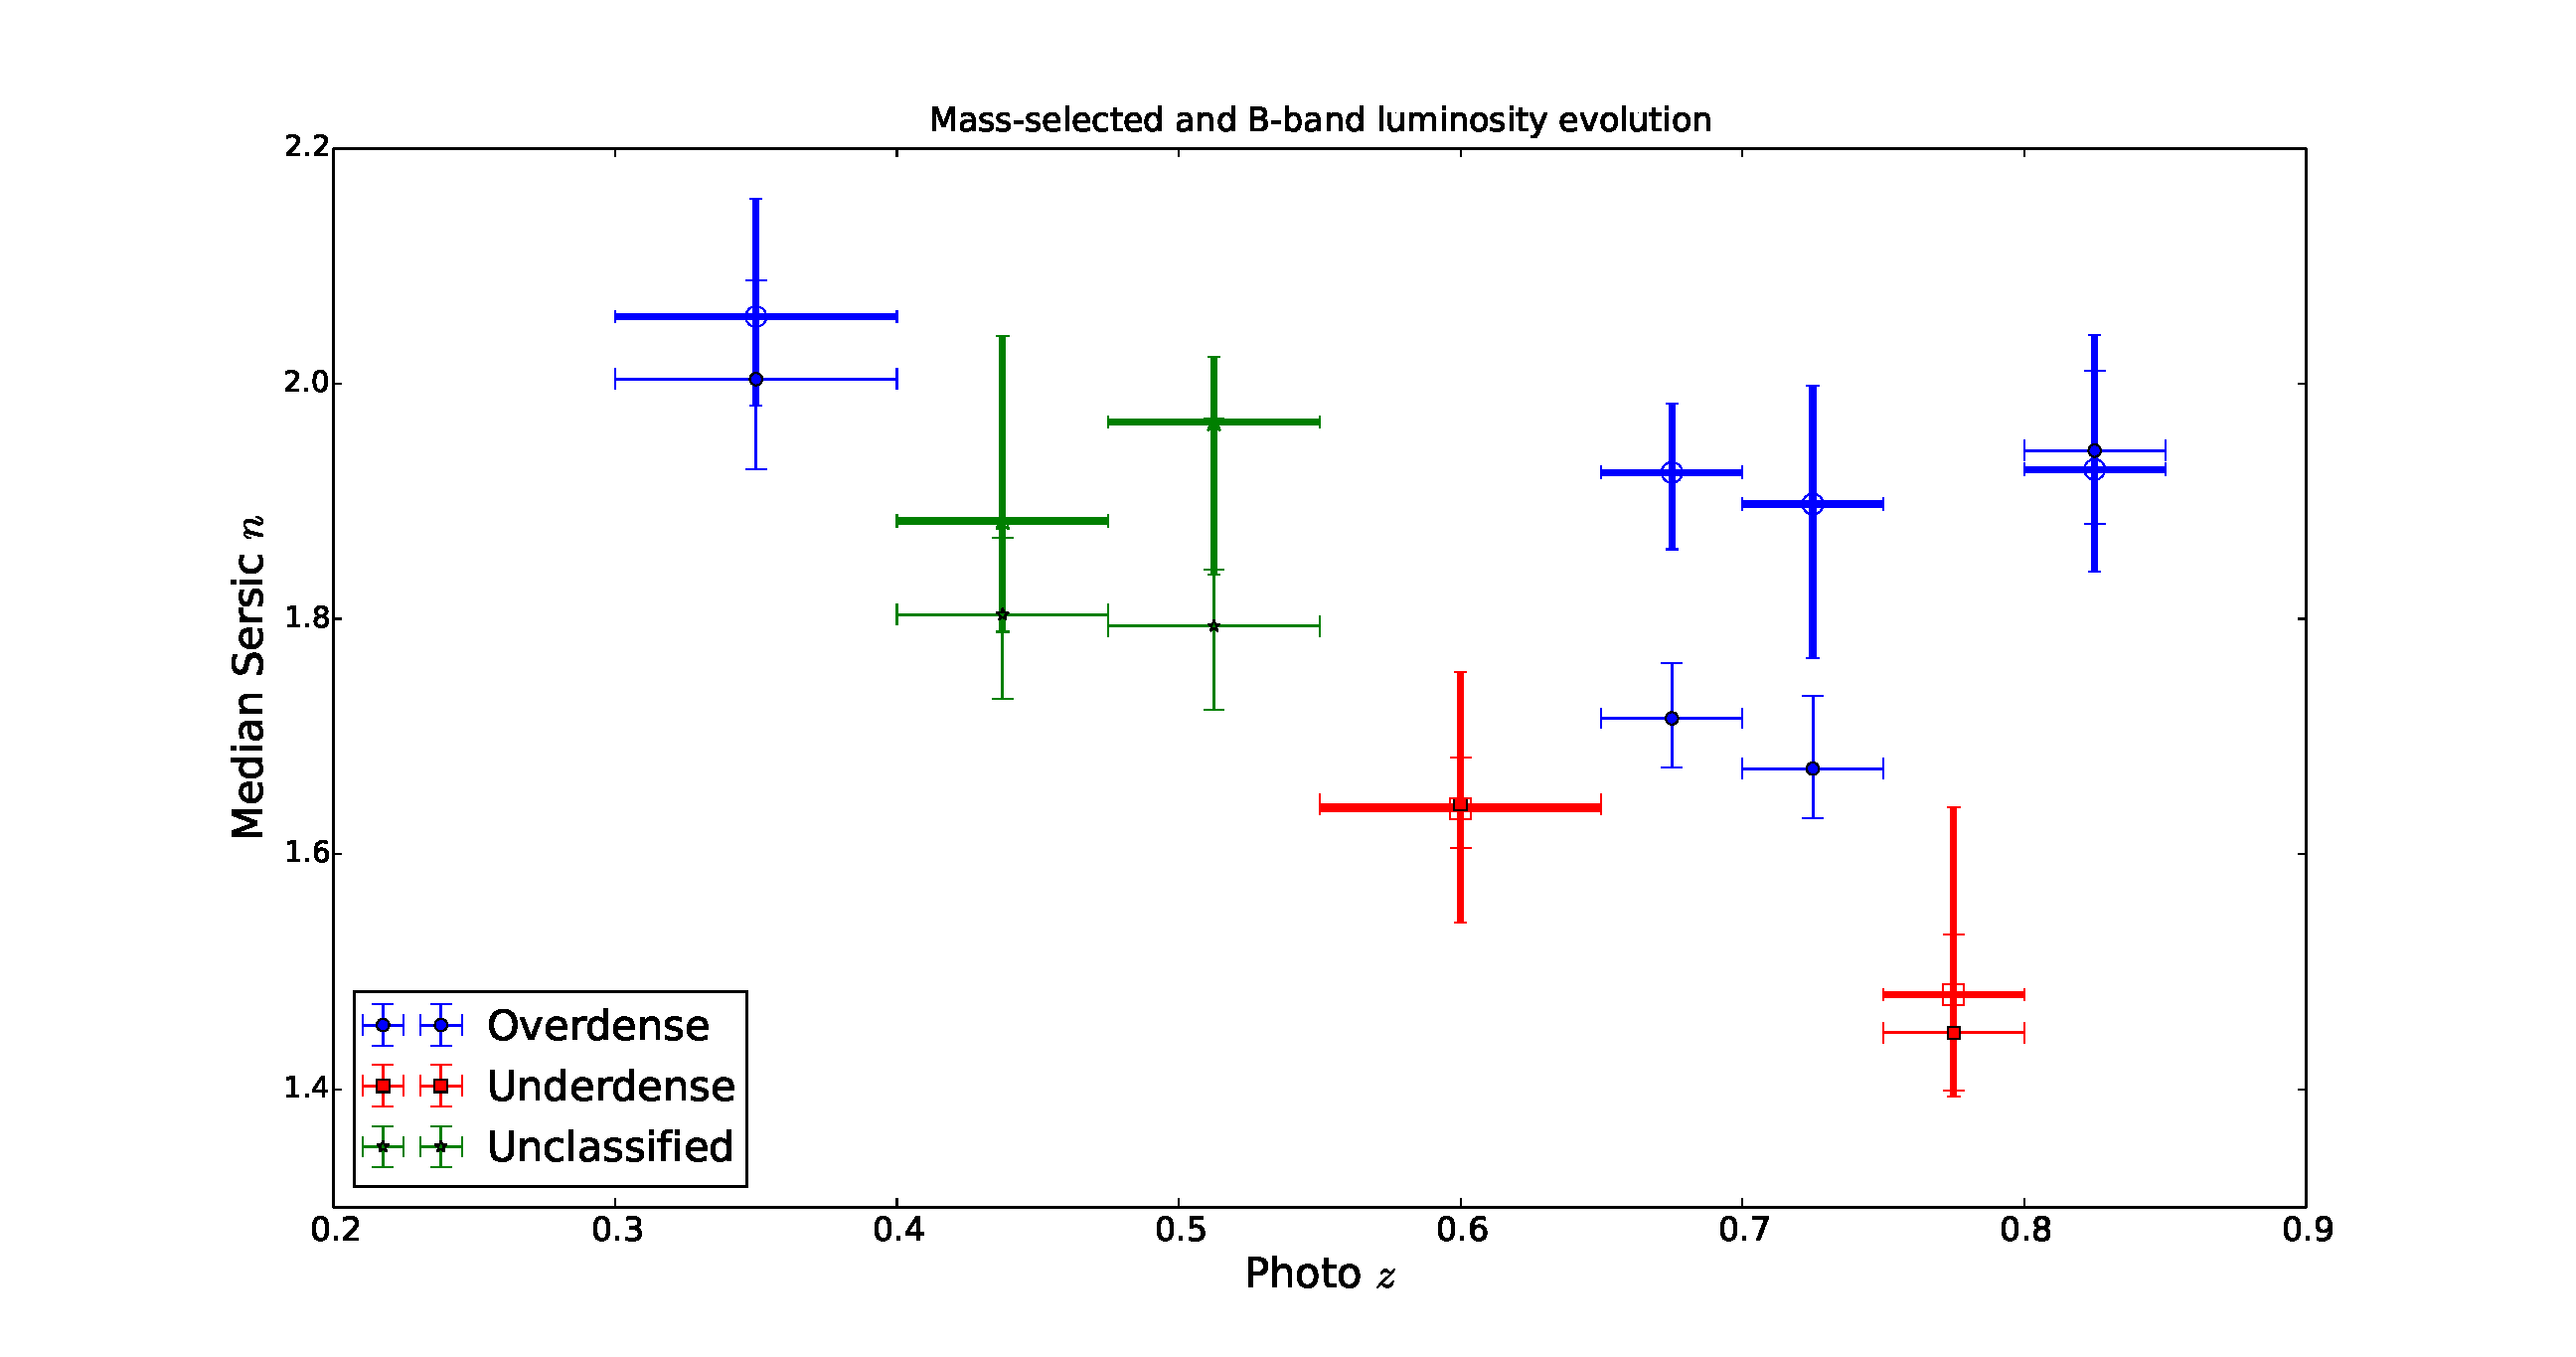
\includegraphics[width=\columnwidth]{median_sersicn}
 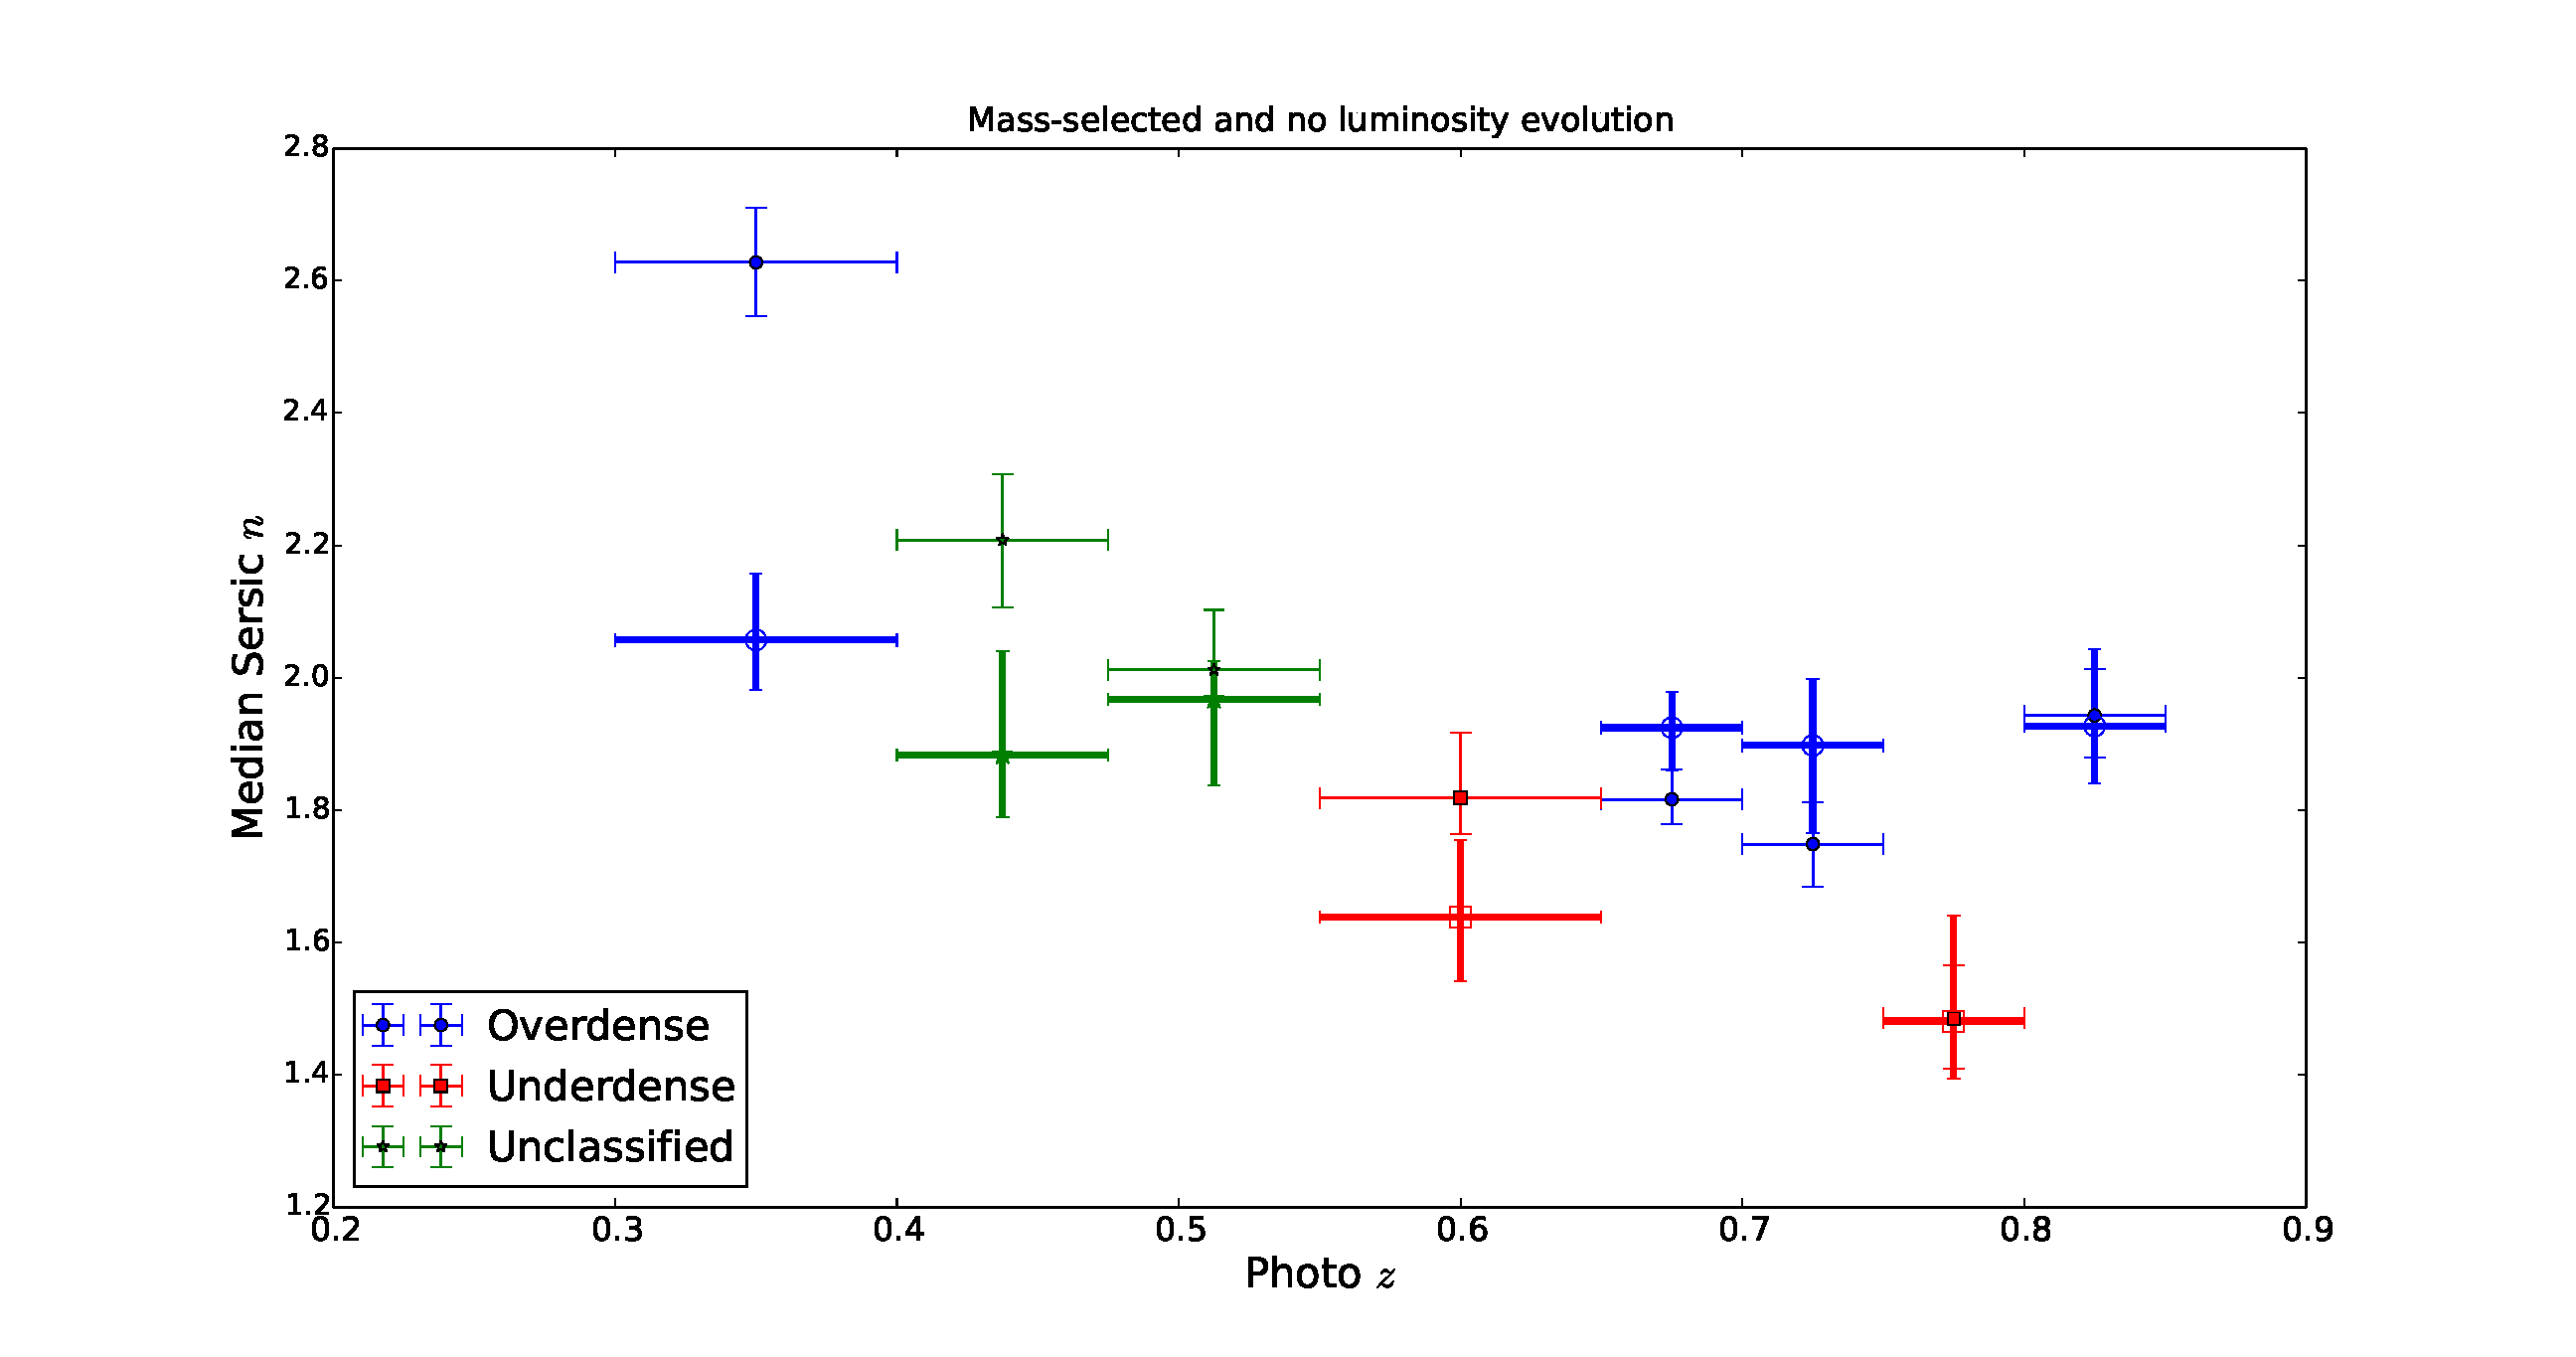
\includegraphics[width=\columnwidth]{median_sersicn(2)}
 \caption{something}
 \label{fig:median_sersicn}
\end{figure*}

\begin{figure*}
 \centering
 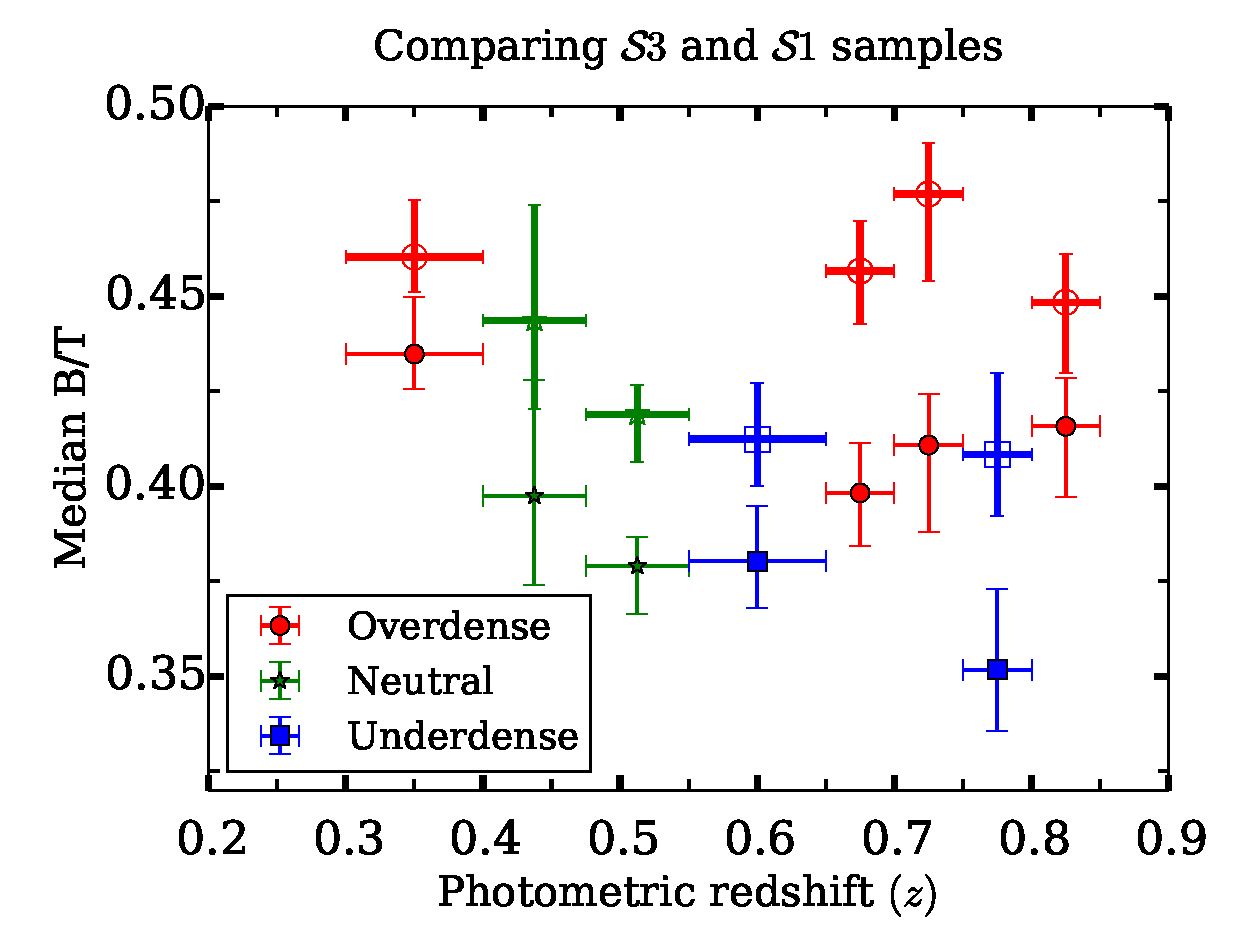
\includegraphics[width=\columnwidth]{median_dvcbtt}
 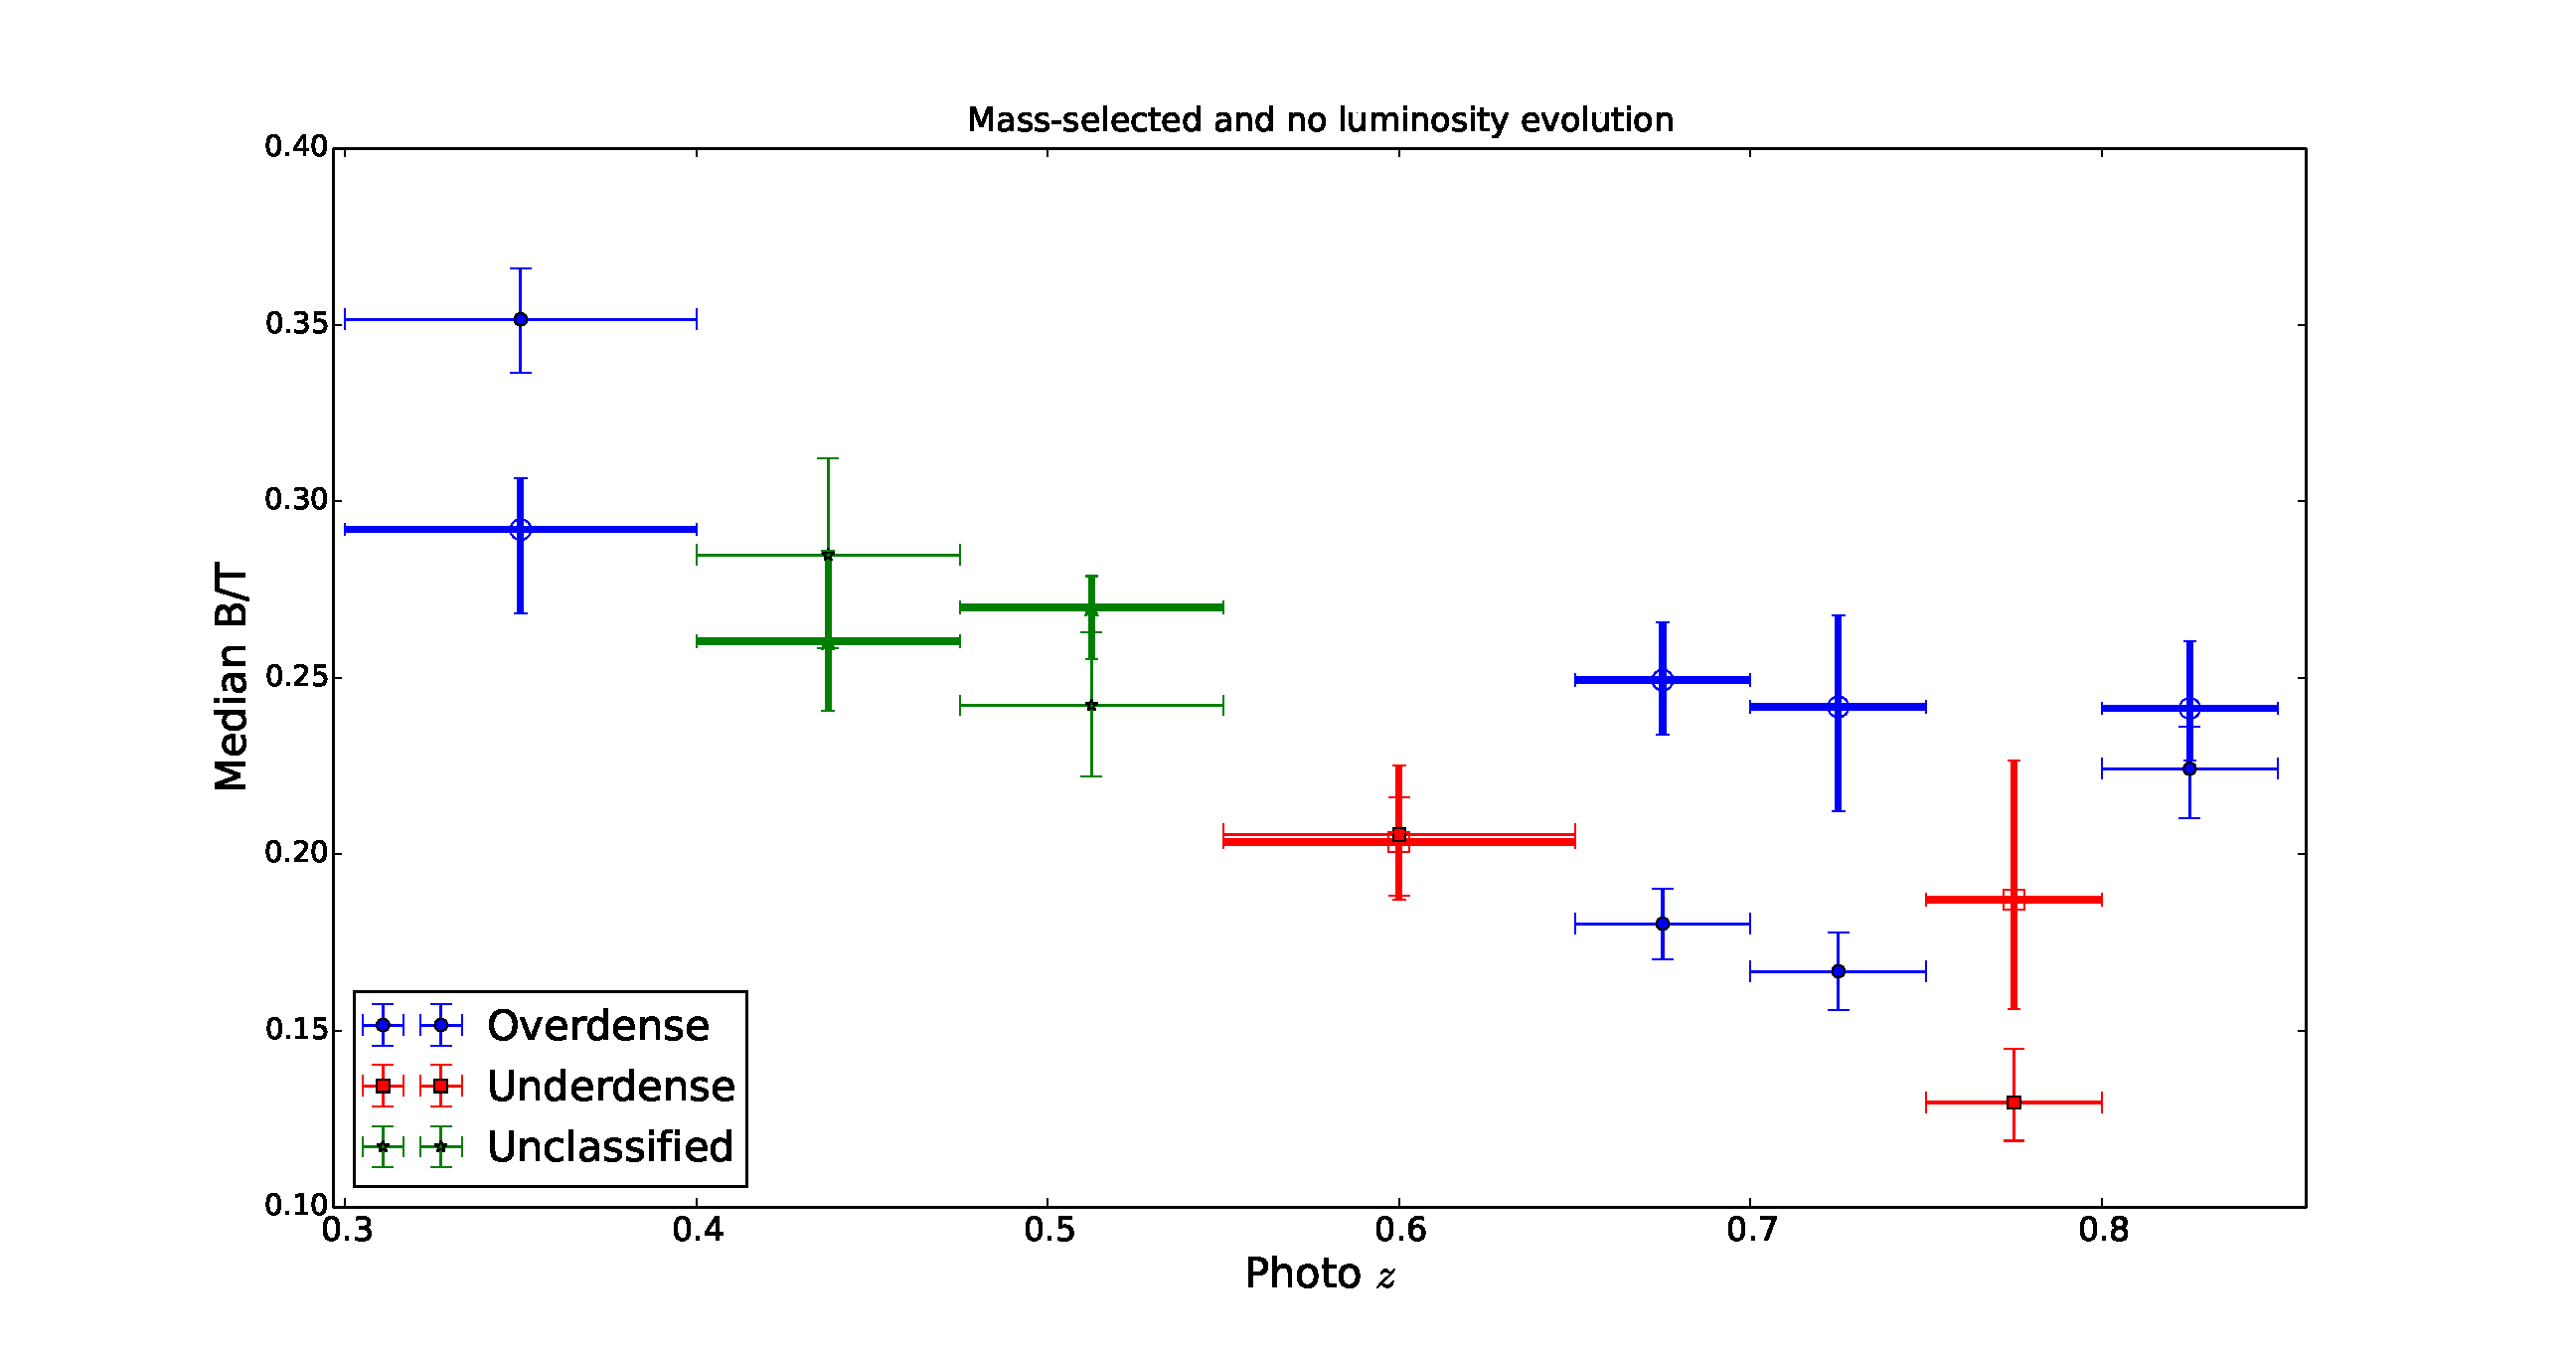
\includegraphics[width=\columnwidth]{median_dvcbtt(2)}
 \caption{something else}
 \label{fig:median_dvcbtt}
\end{figure*}

\section{Conclusion}
\label{S:conclusion}

We have shown that 
\section*{Acknowledgments}

AK and RM acknowledge the support of NASA ROSES 12-EUCLID12-0004, and
program HST-AR-12857.01-A, provided by NASA through a grant from the
Space Telescope Science Institute, which is operated by the
Association of Universities for Research in Astronomy, Incorporated,
under NASA contract NAS5-26555. AK and RM thank Alexie Leauthaud for many useful discussions.

%\begin{thebibliography}
\bibliography{ref}
%\end{thebibliography}

\begin{figure}
 \centering
 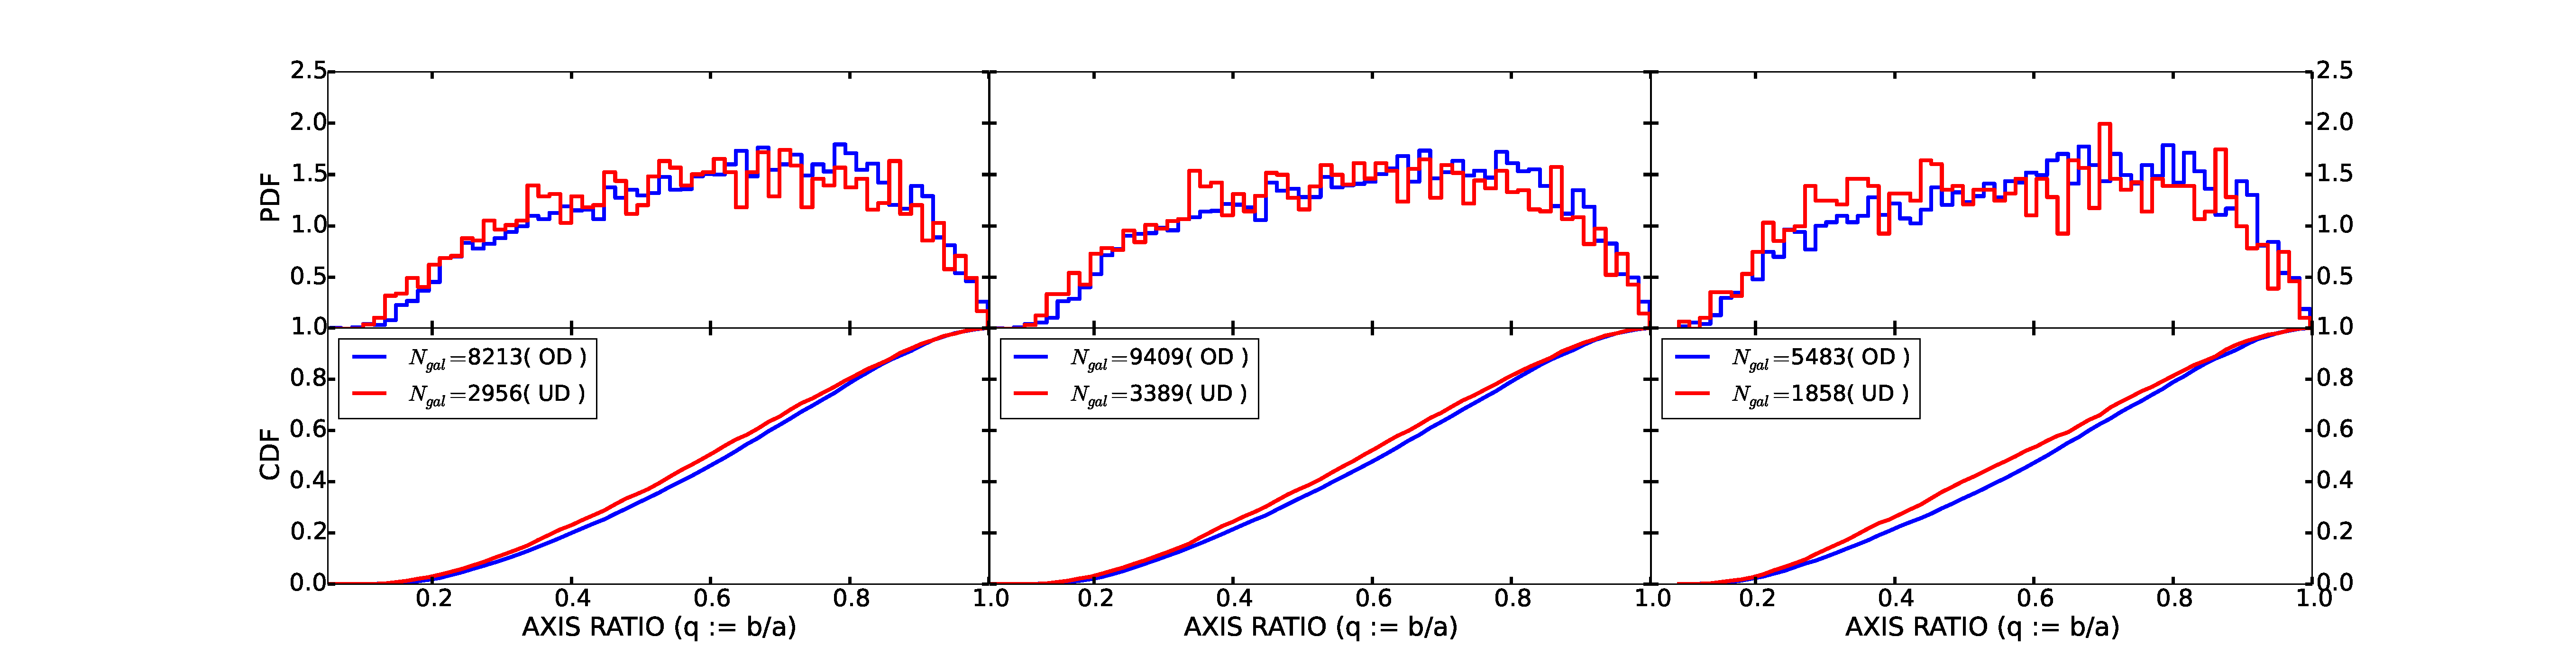
\includegraphics[width=\columnwidth]{axis_ratio_all.eps}
 \caption{KS p-value = 0.004 \& AD p-value = 0.001}
 \label{fig:axisratio_all}
\end{figure}


\begin{figure*}
 \centering
 a) 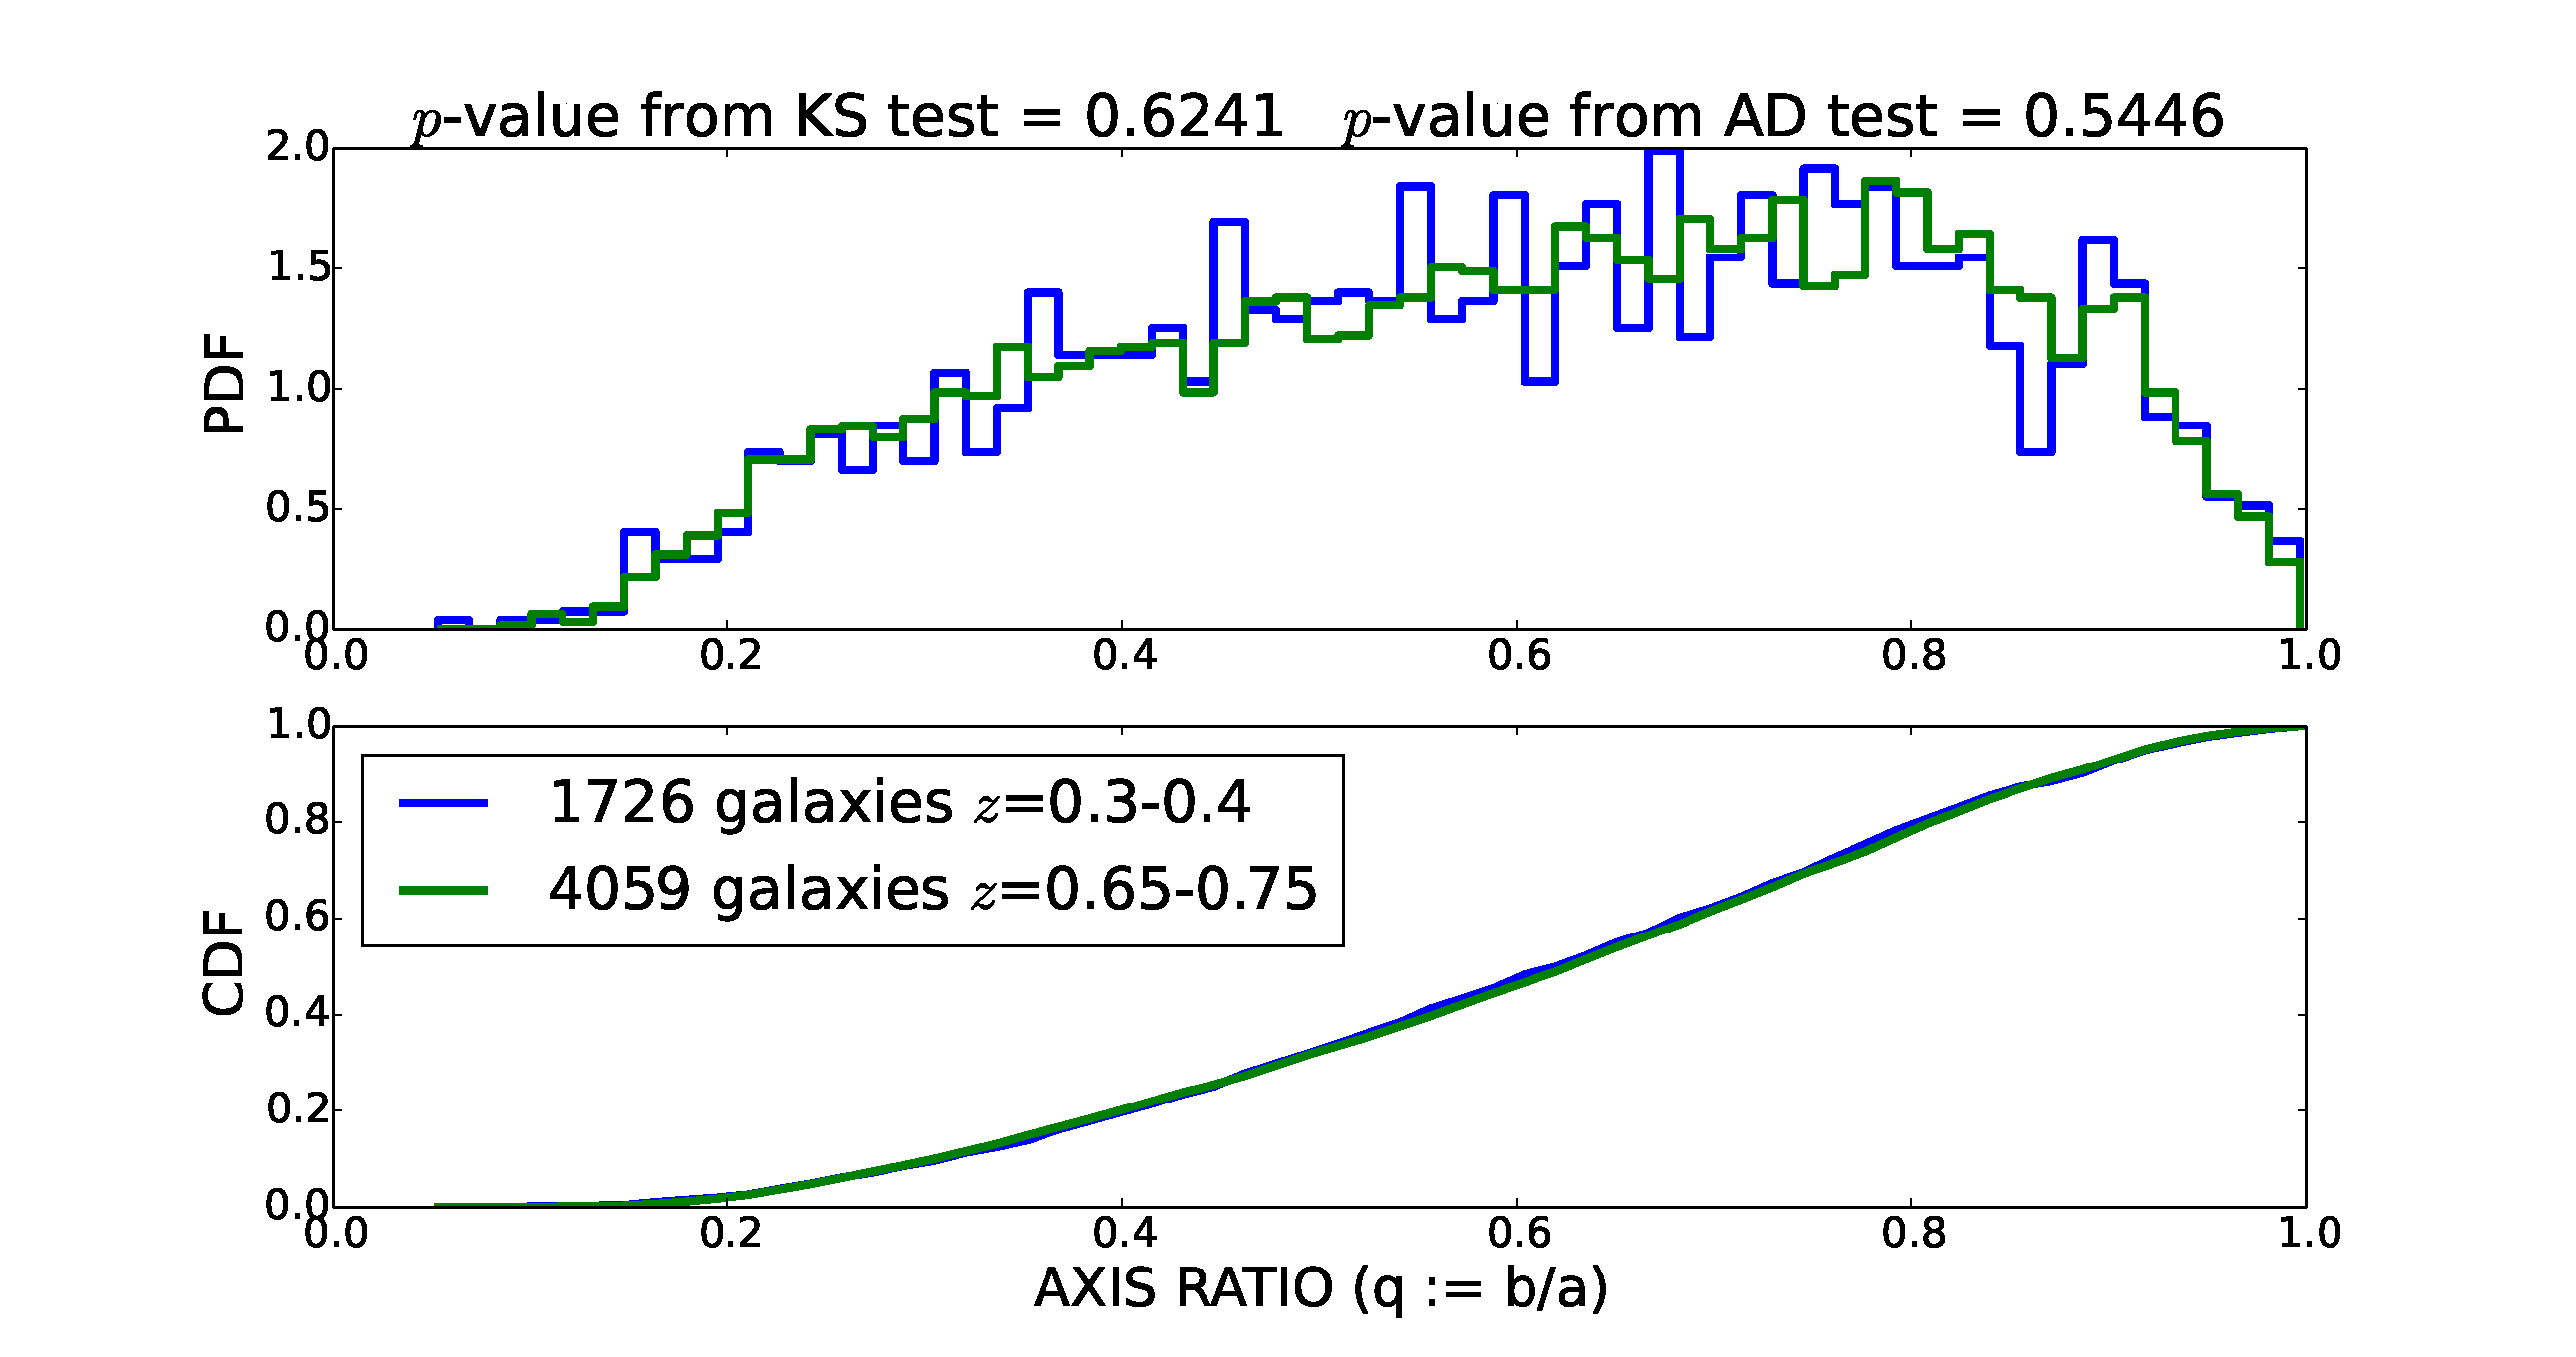
\includegraphics[width=0.9\columnwidth]{axisratio(0)_0dot3-0dot4_0dot65-0dot75.eps} \
 b) 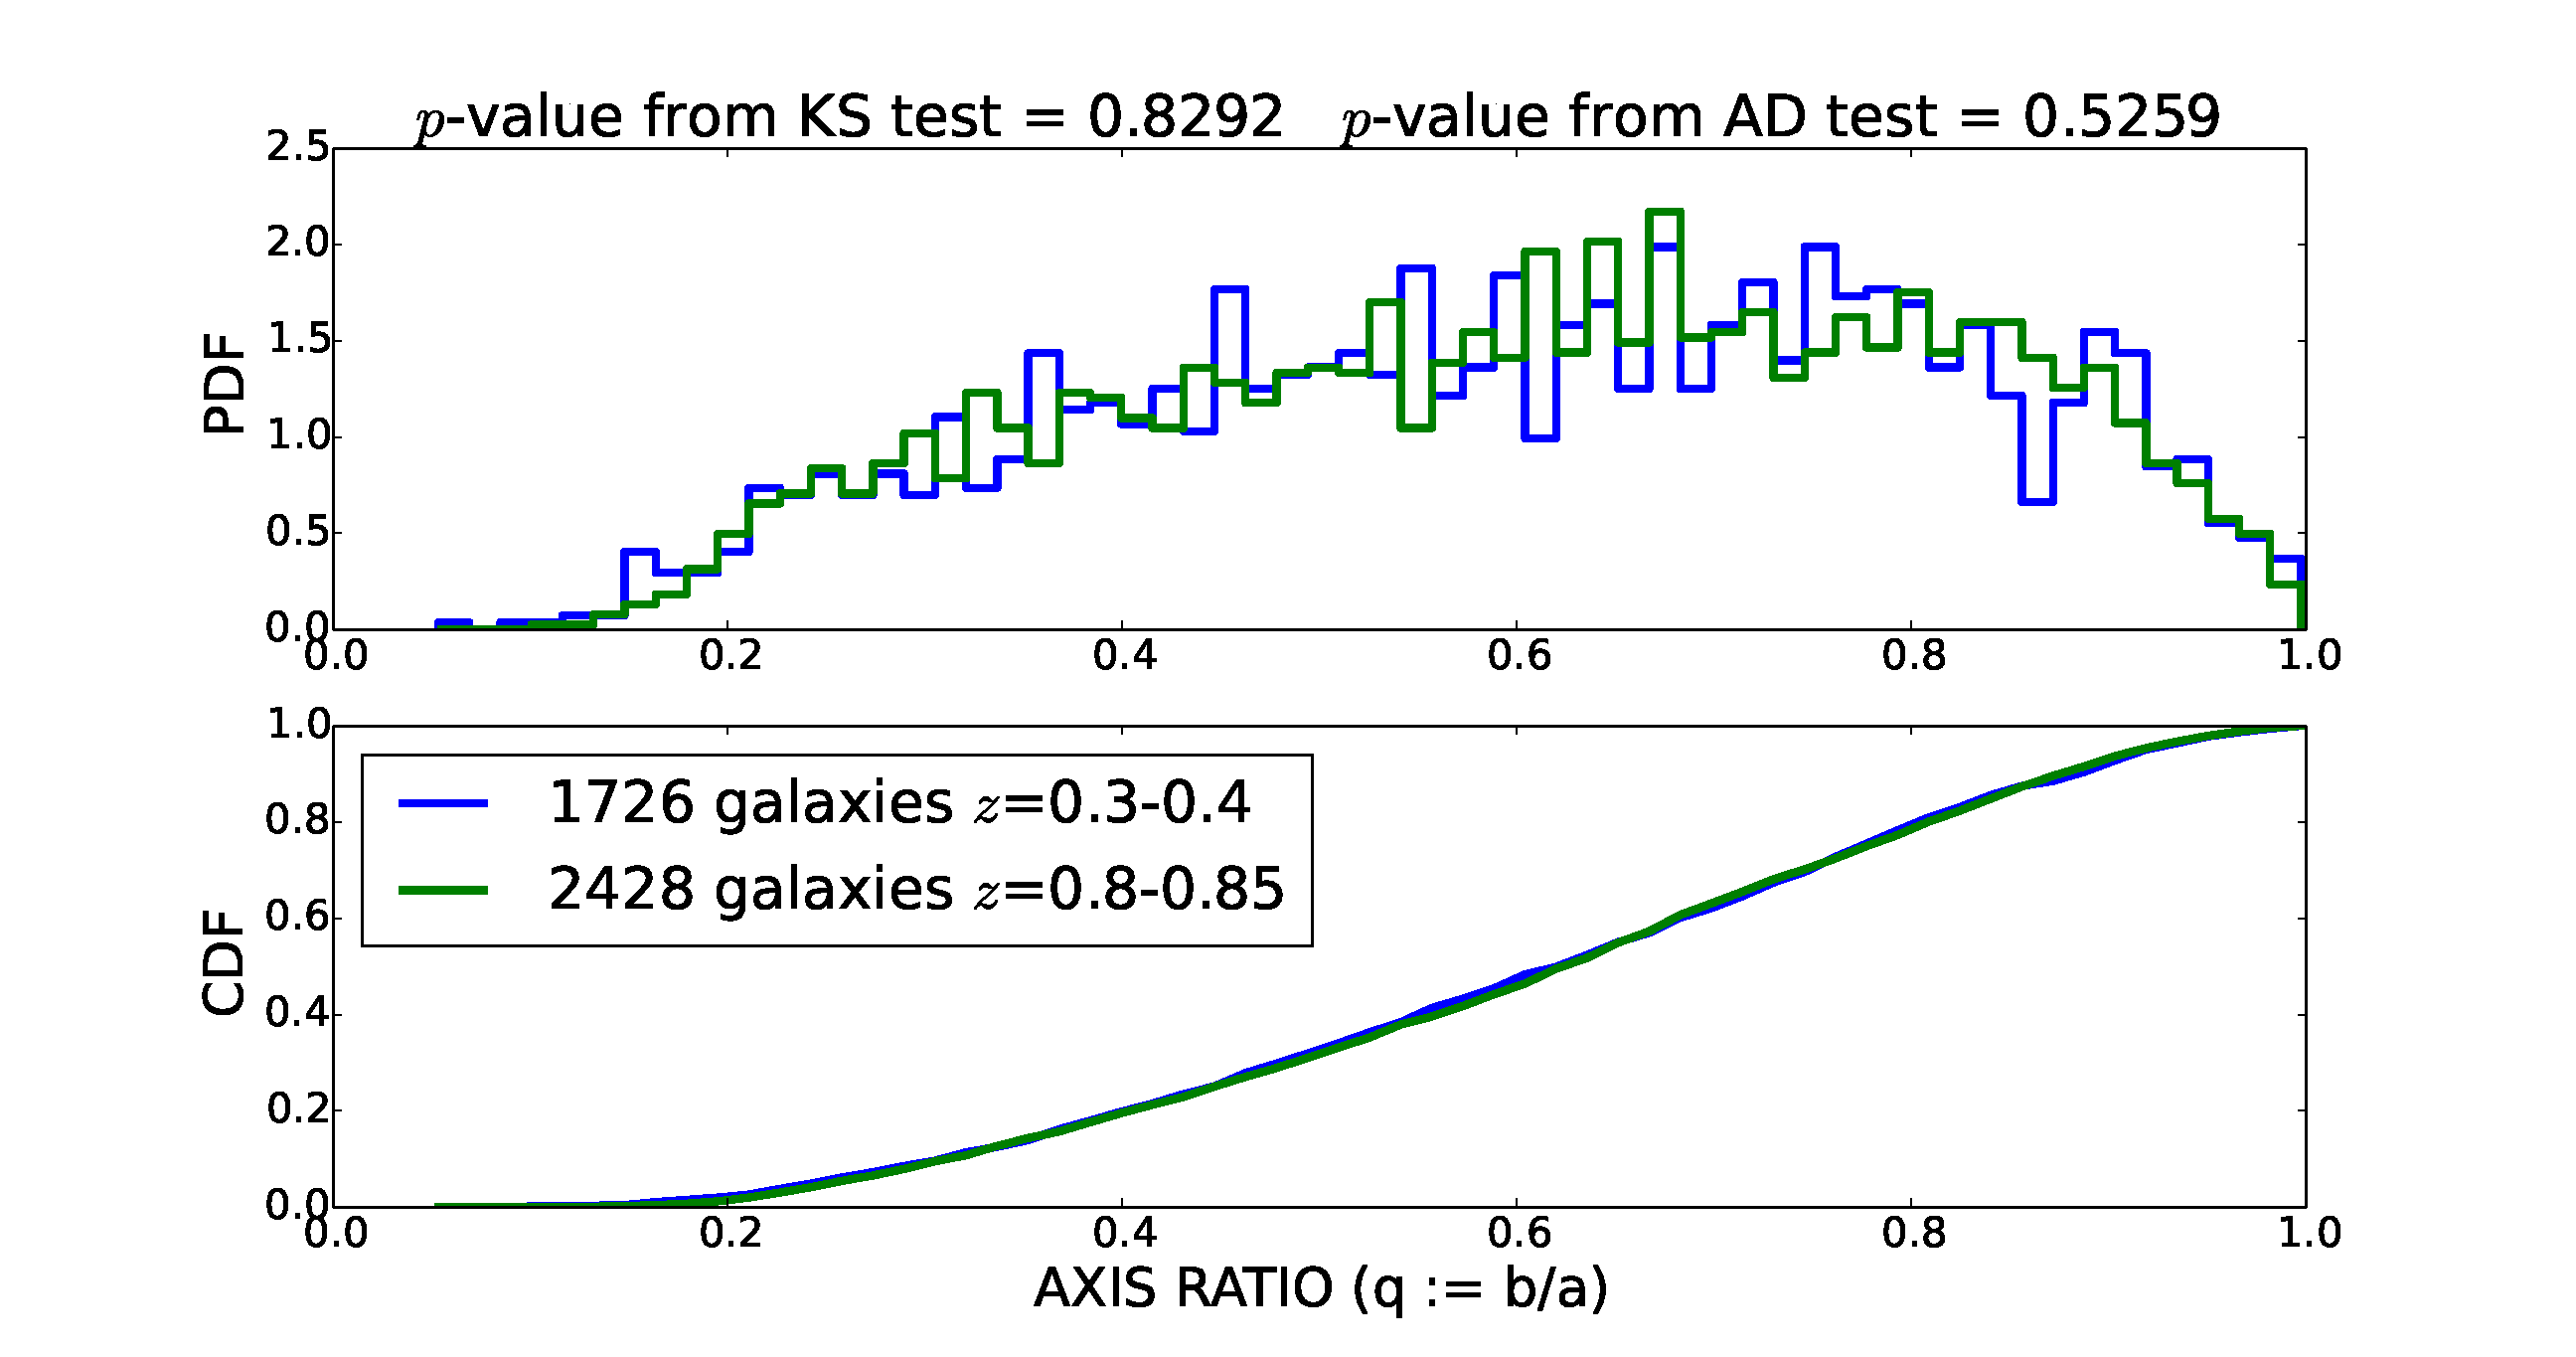
\includegraphics[width=0.9\columnwidth]{axisratio(0)_0dot3-0dot4_0dot80-0dot85.eps} \\
 c) 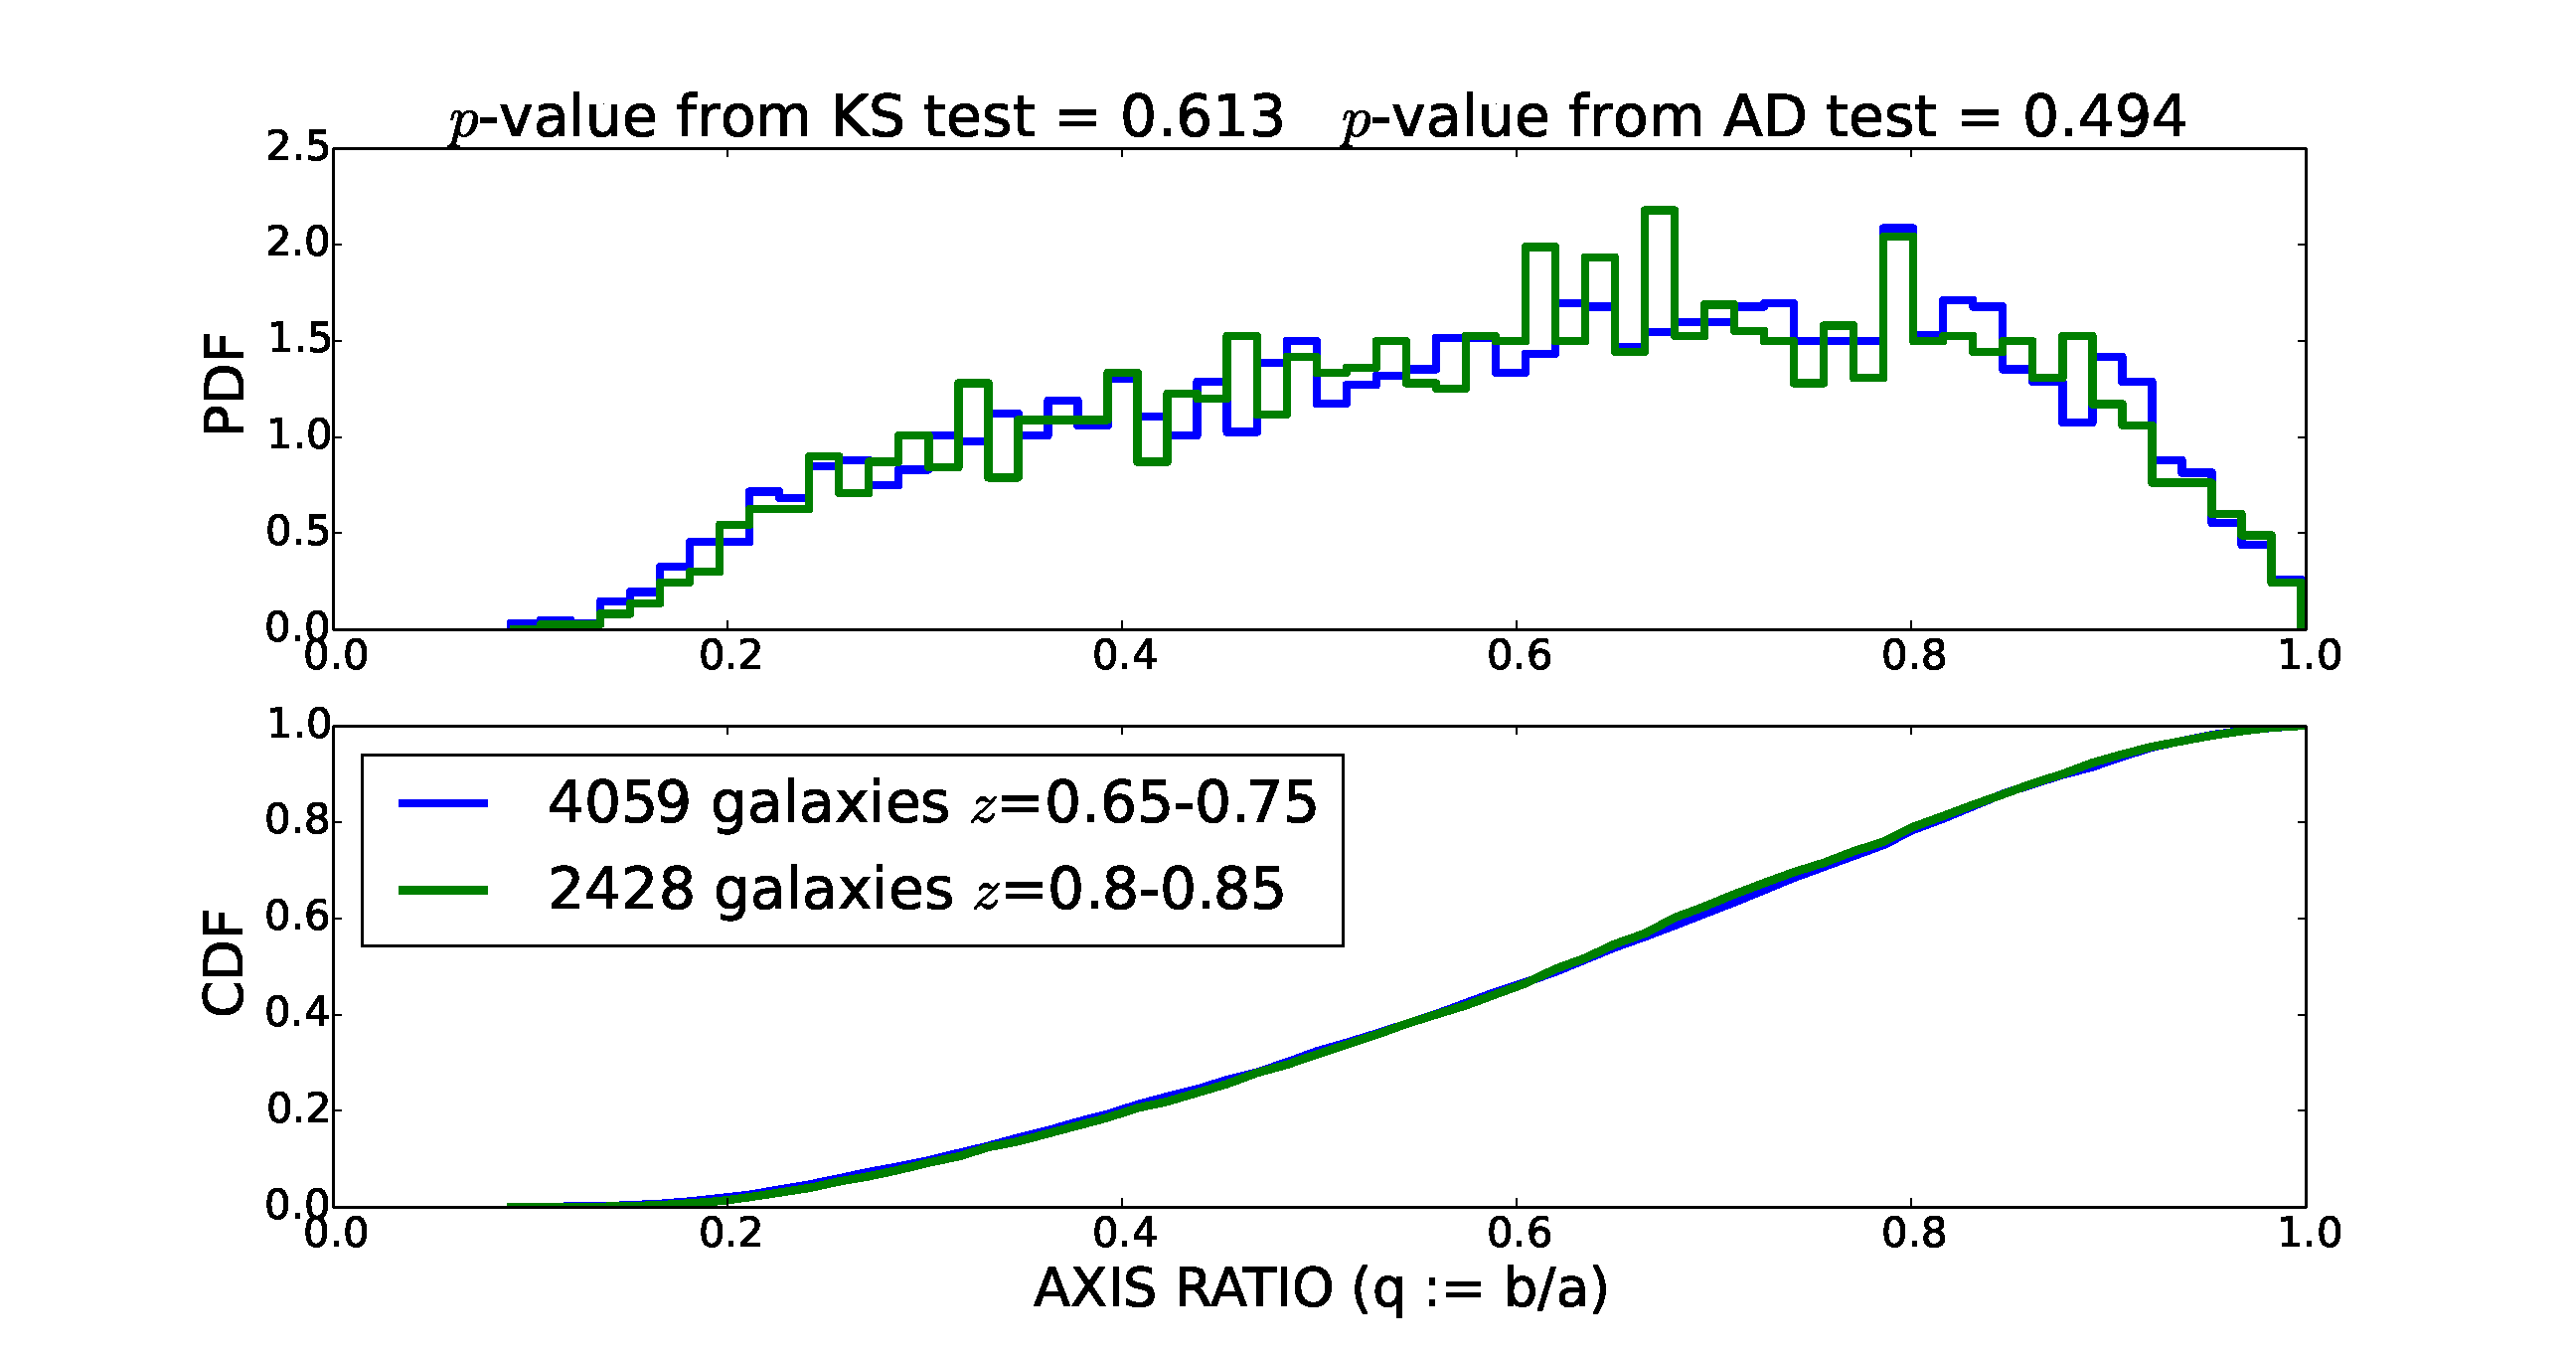
\includegraphics[width=0.9\columnwidth]{axisratio(0)_0dot65-0dot75_0dot80-0dot85.eps} \
 d) 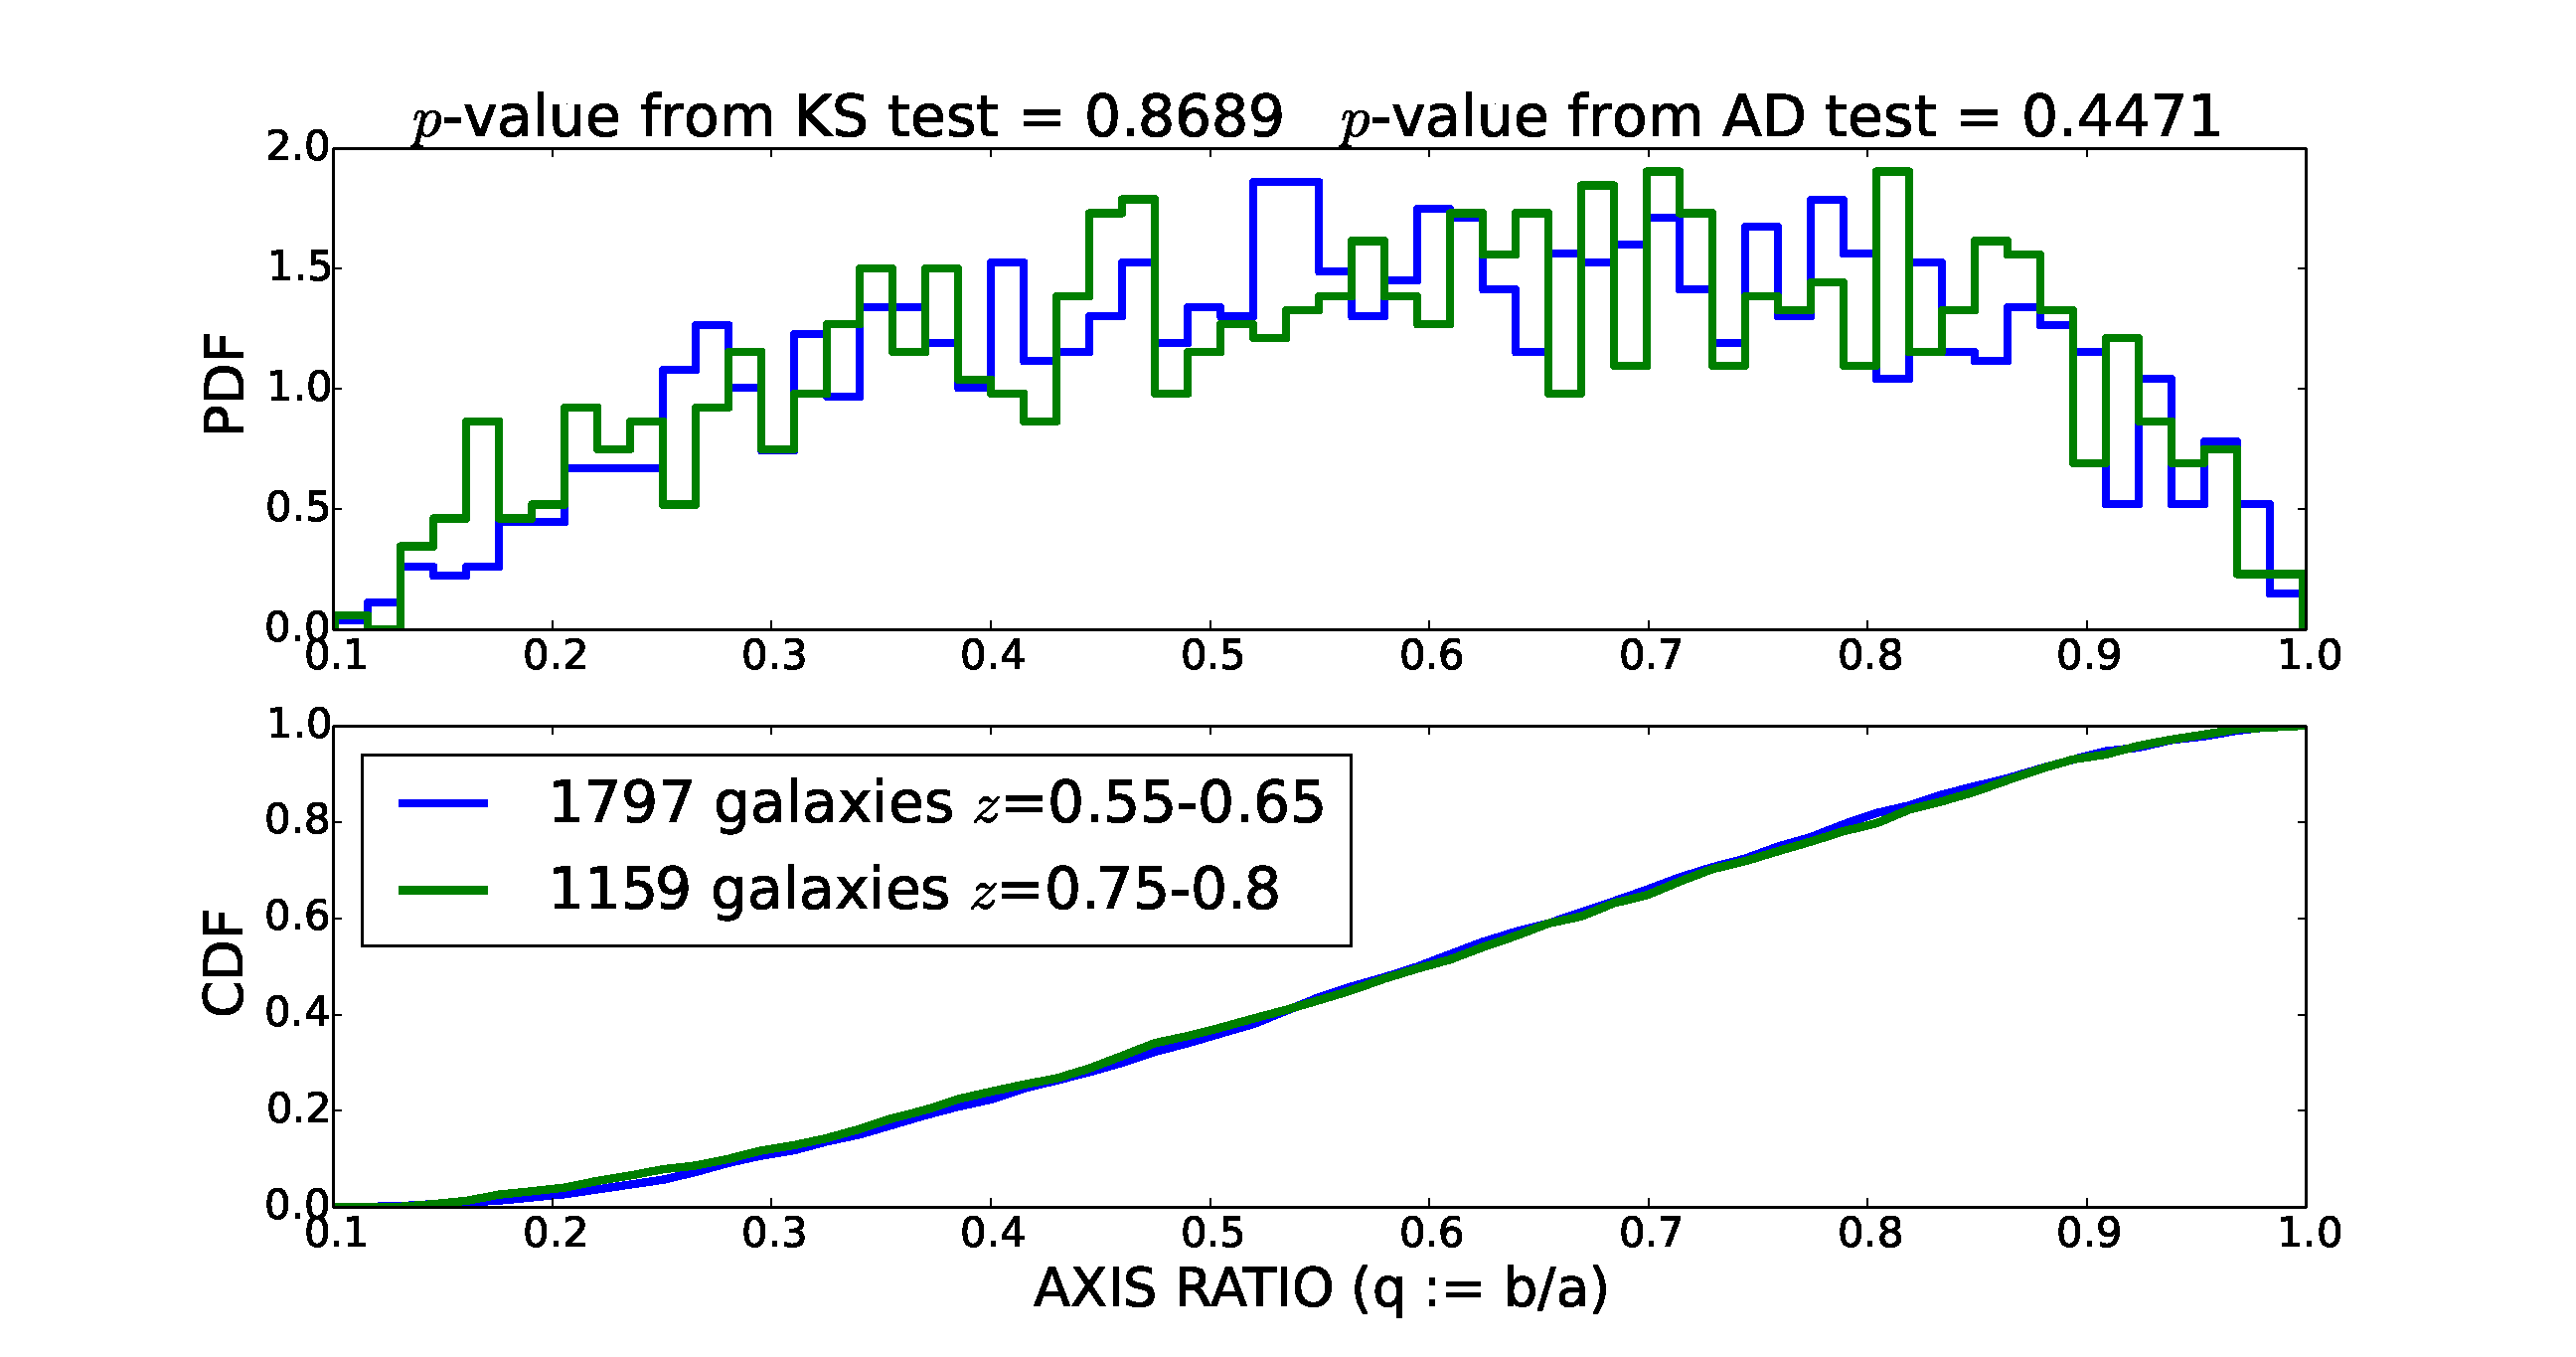
\includegraphics[width=0.9\columnwidth]{axisratio(0)_0dot55-0dot65_0dot75-0dot8.eps} \
 \caption{Comparison of axis ratios of galaxies in similar environments. $p$-values from the KS and AD test are (will be) given in the plot.}
 \label{fig:axisratio_similar}
\end{figure*}

\begin{figure*}
 \centering
 a) 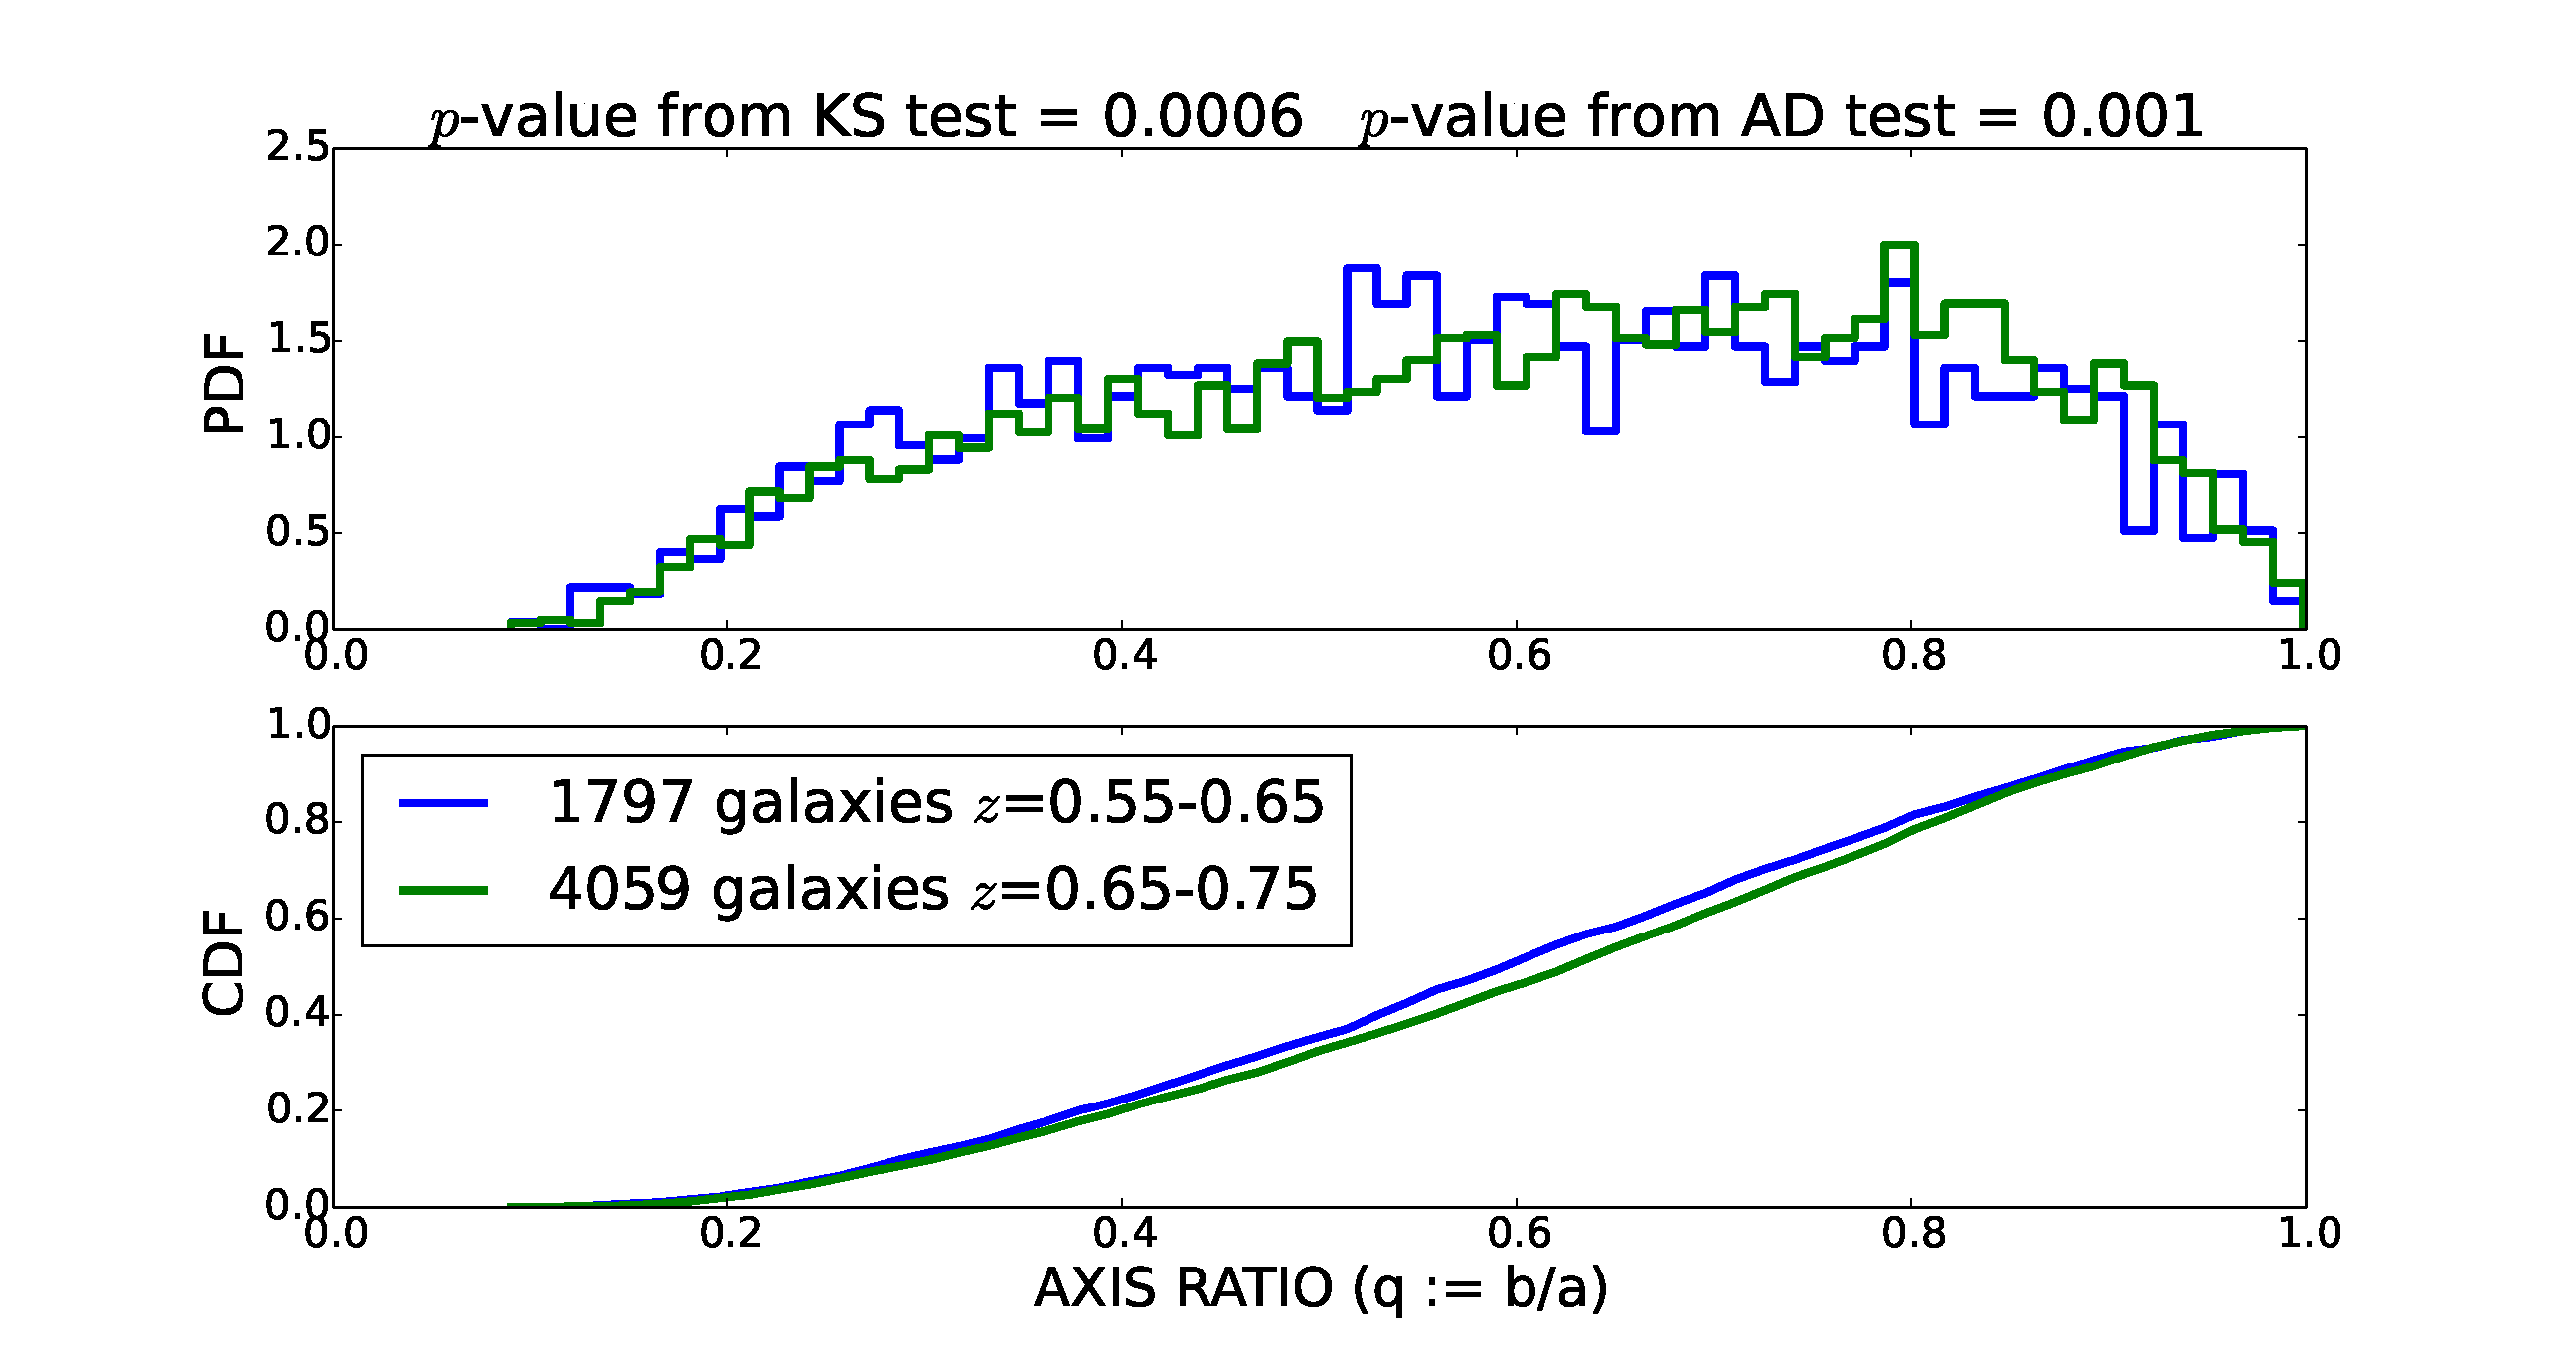
\includegraphics[width=0.9\columnwidth]{axisratio(0)_0dot55-0dot65_0dot65-0dot75.eps} \
 b) 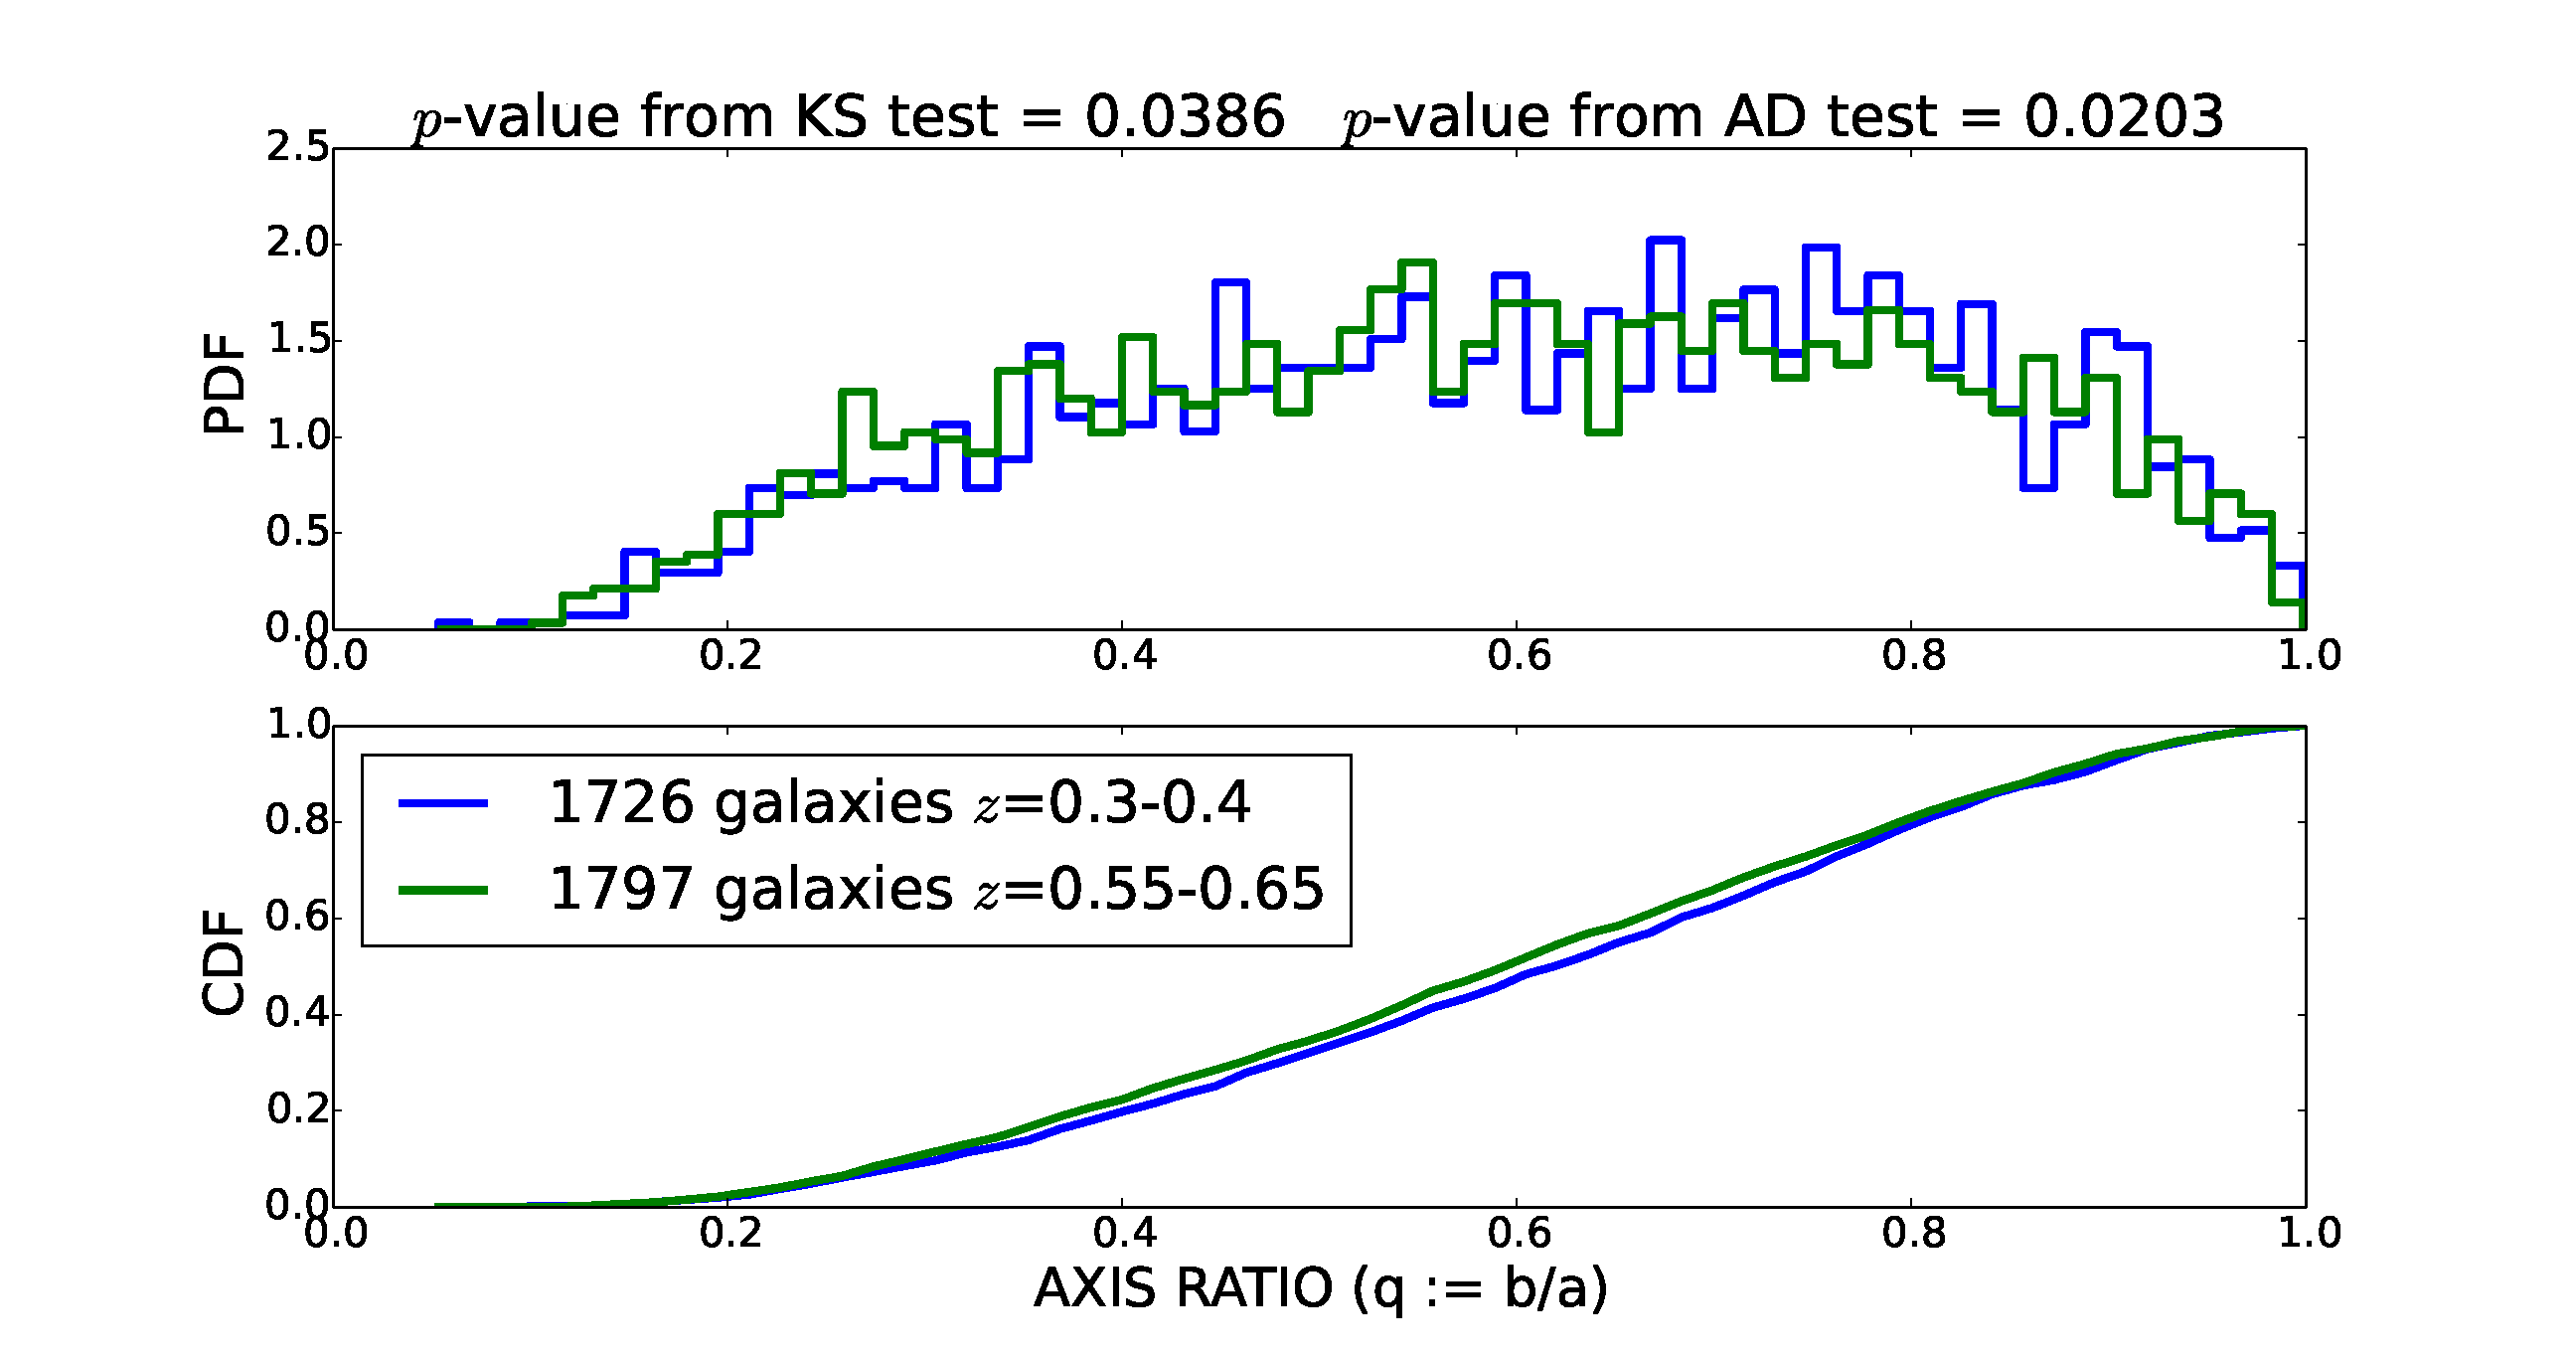
\includegraphics[width=0.9\columnwidth]{axisratio(0)_0dot3-0dot4_0dot55-0dot65.eps} \\
 c) 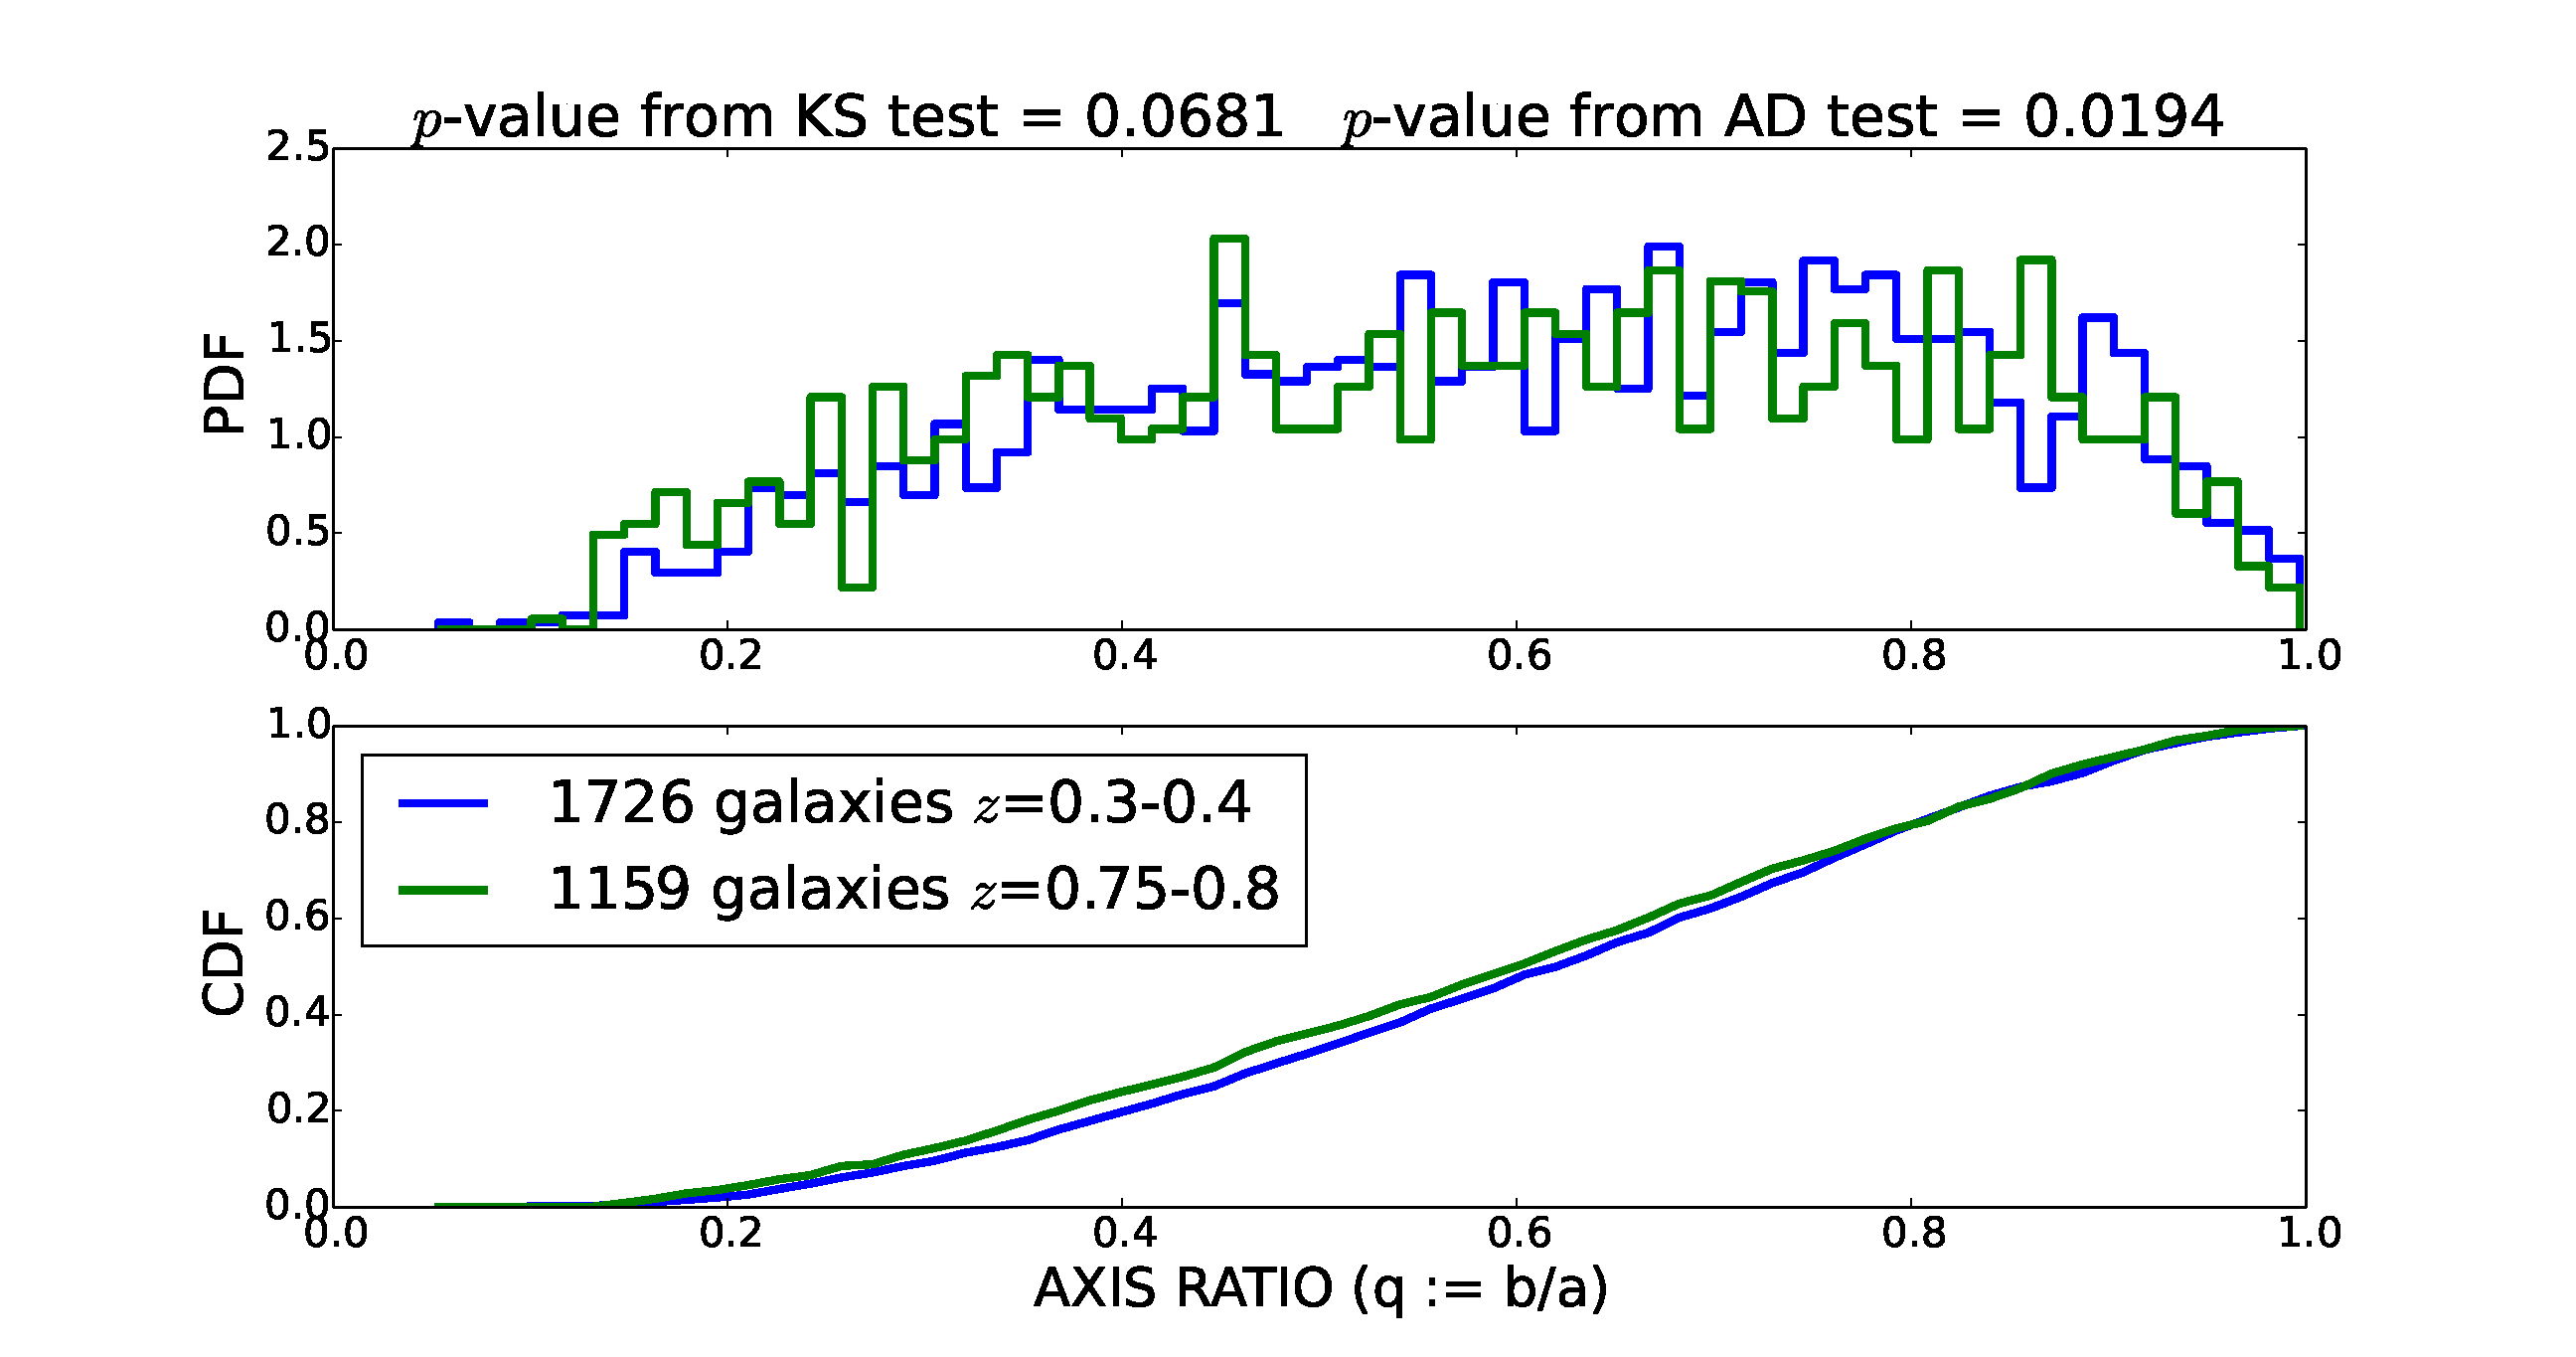
\includegraphics[width=0.9\columnwidth]{axisratio(0)_0dot3-0dot4_0dot75-0dot8.eps} \
 d) 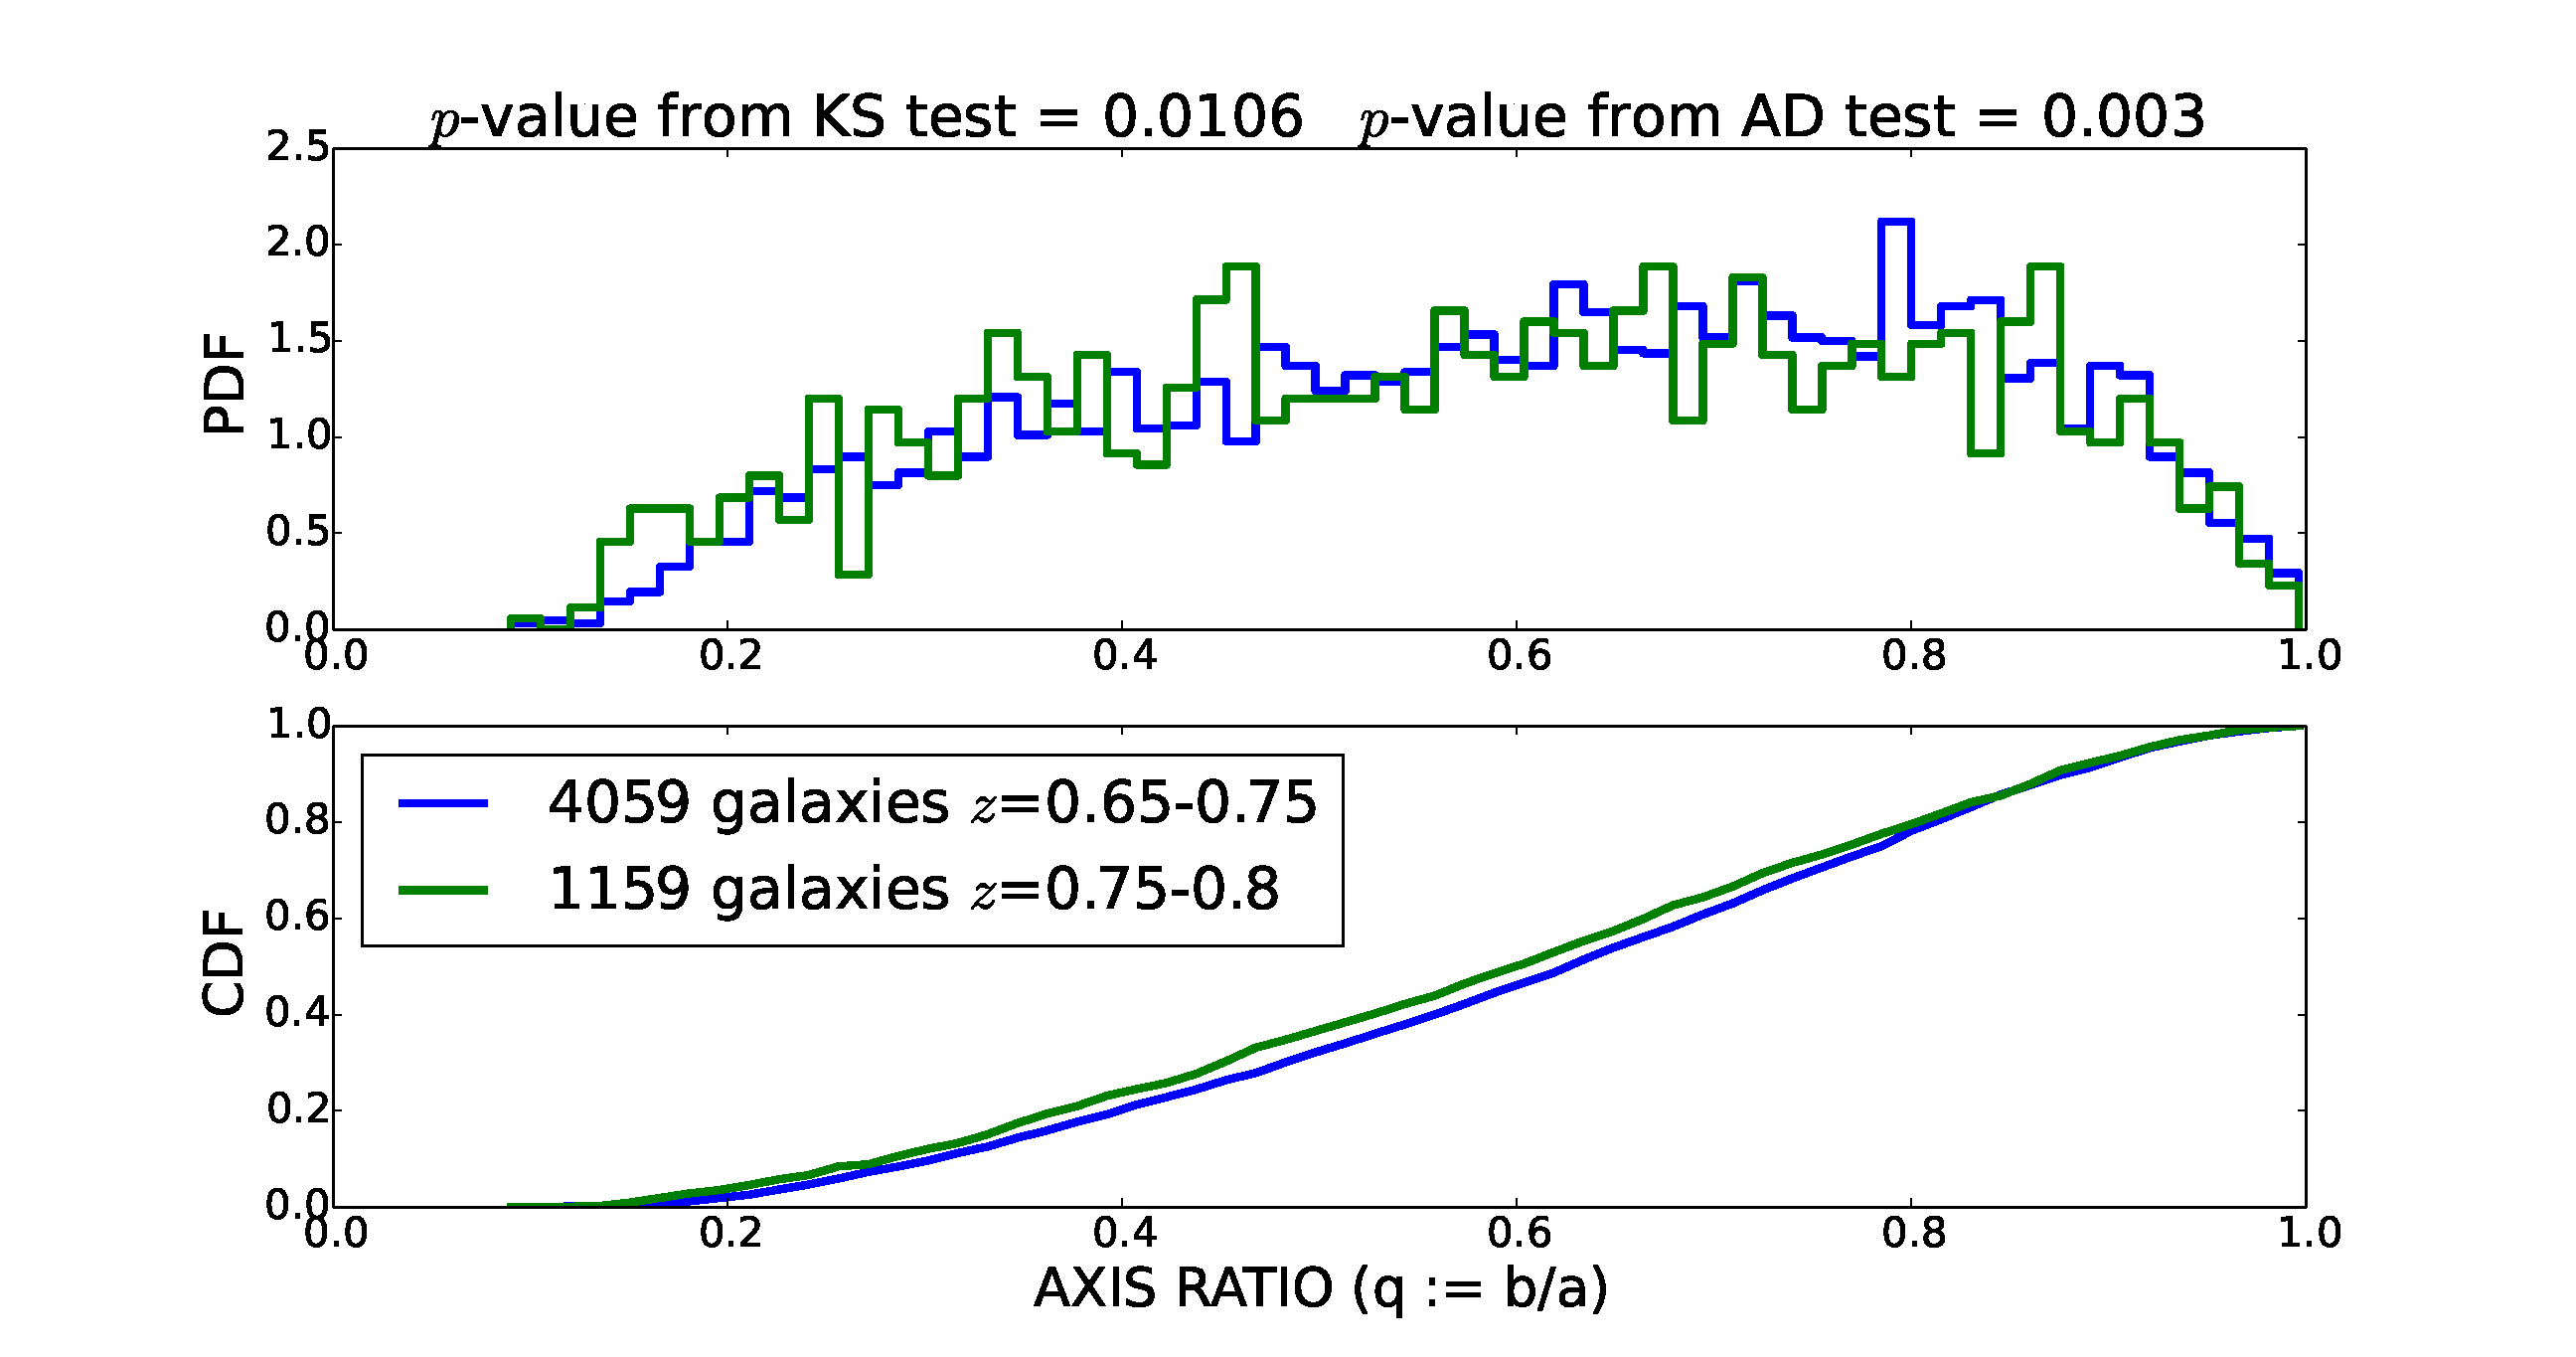
\includegraphics[width=0.9\columnwidth]{axisratio(0)_0dot65-0dot75_0dot75-0dot80.eps} \
 \caption{Comparison of axis ratios of galaxies in contrasting environments. $p$-values from the KS and AD test are (will be) given in the plot.}
 \label{fig:axisratio_contrasting}
\end{figure*}


\begin{figure*}
 \centering
 a) 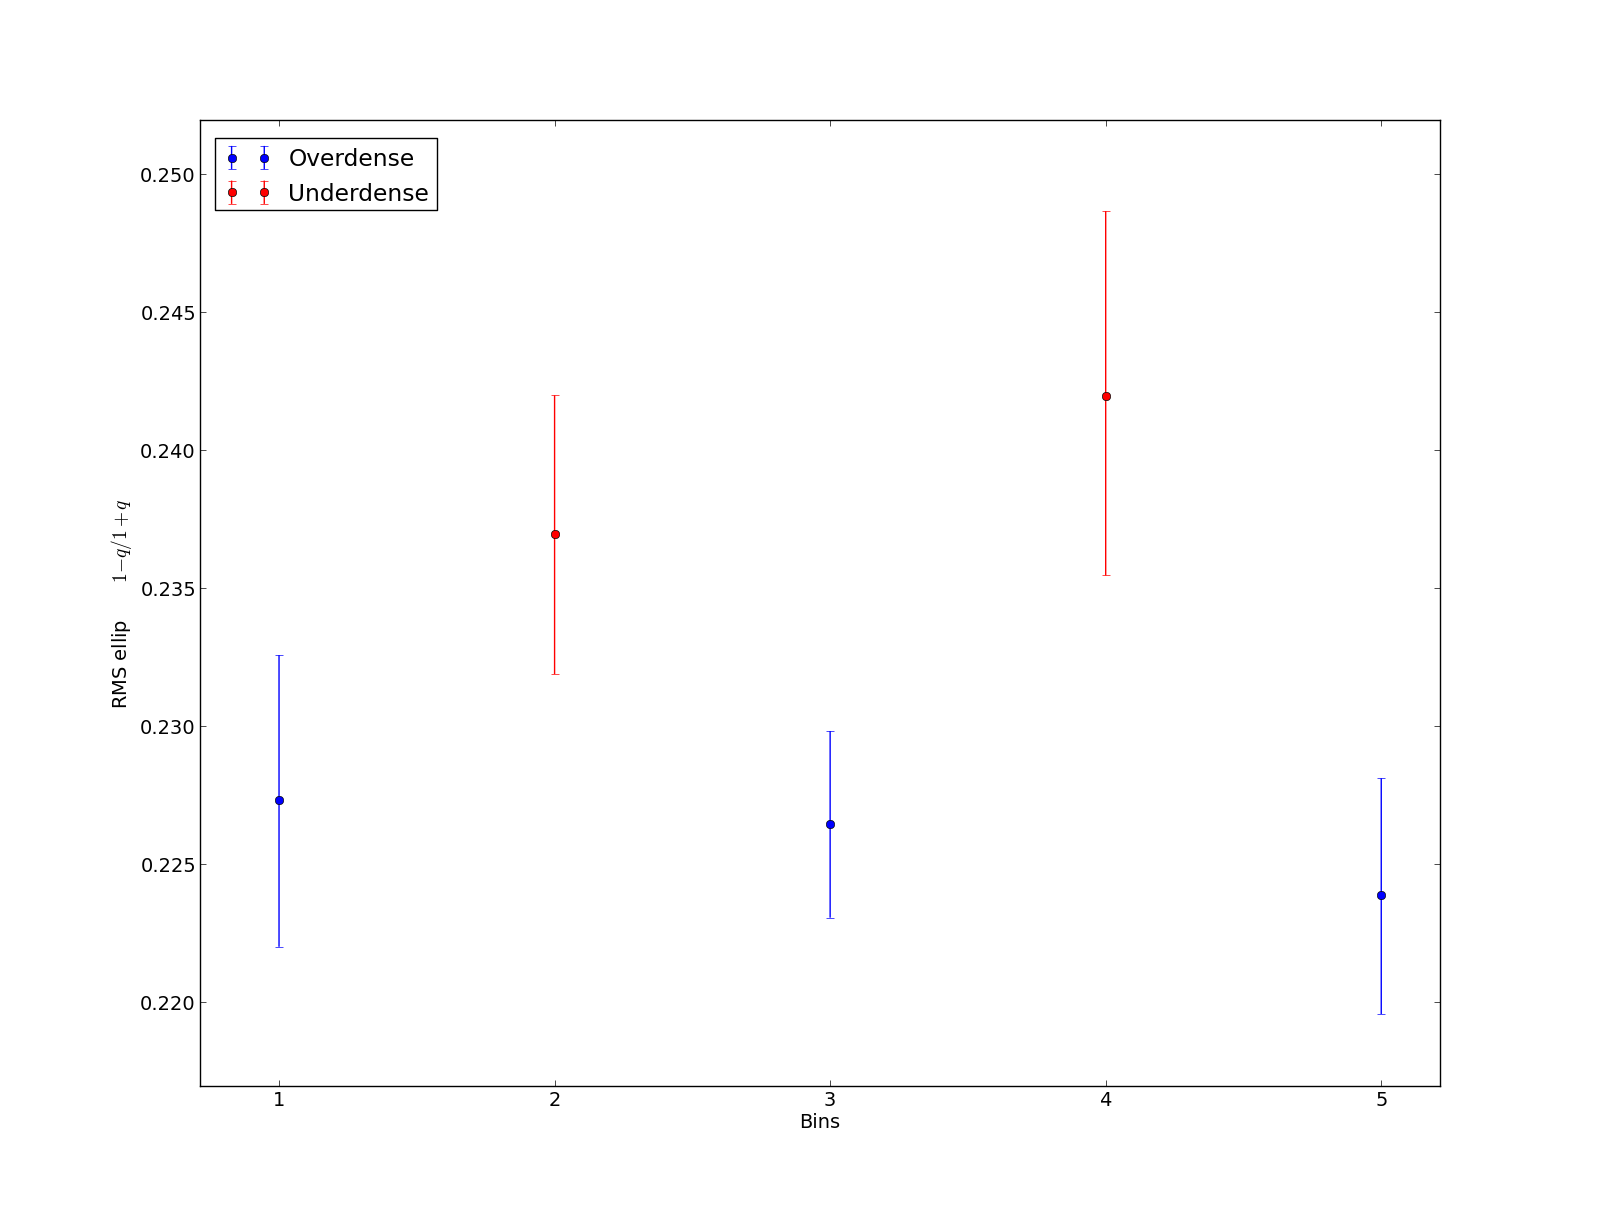
\includegraphics[width=0.9\columnwidth]{rms_ellip1.eps} \
 b) 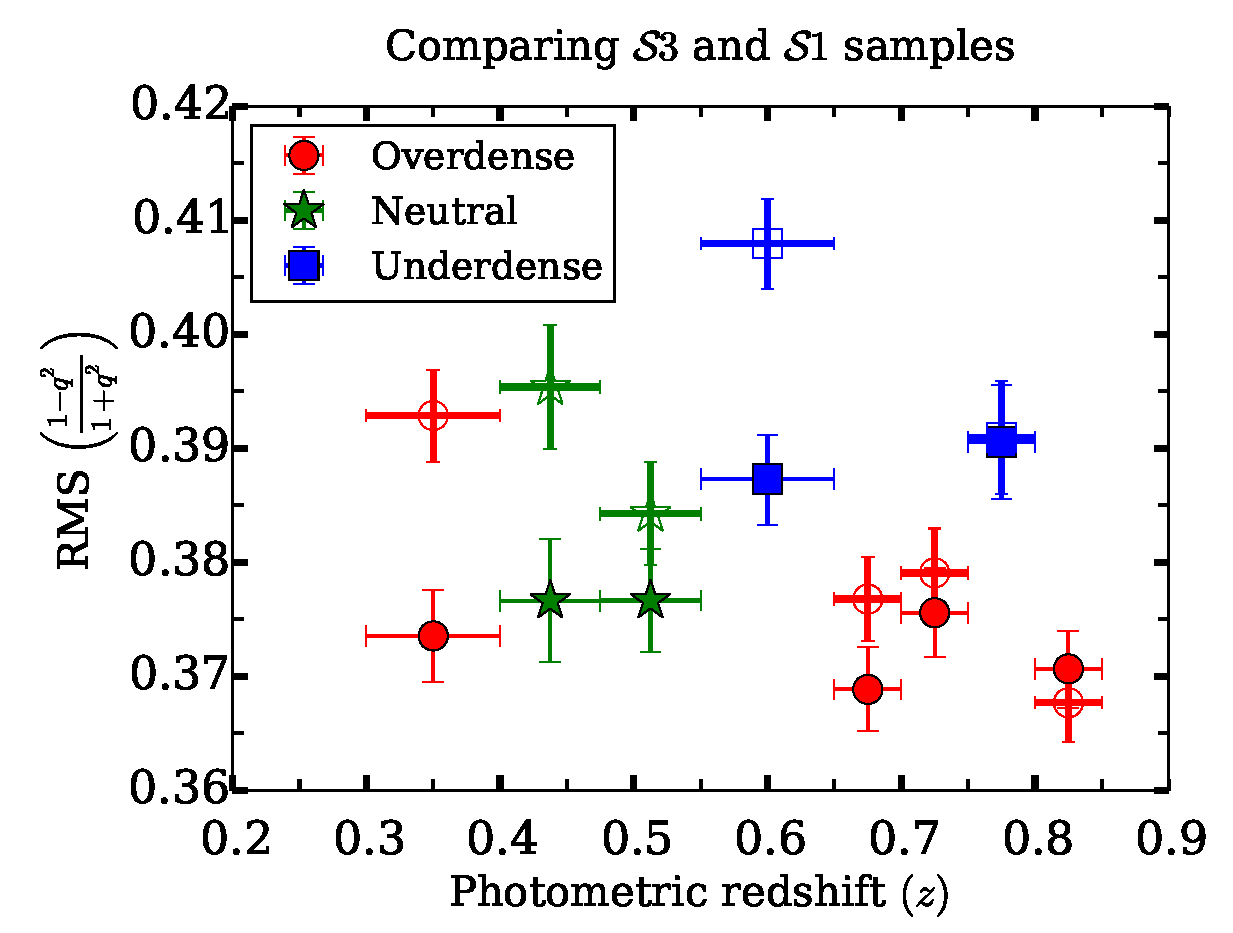
\includegraphics[width=0.9\columnwidth]{rms_ellip2_noevolution.eps} \\
 \caption{Left: RMS ellipticities with ellipticity defined as $\frac{1-q}{1+q}$. \; 
          Right: RMS ellipticities with ellipticity defined as $\frac{1-q^2}{1+q^2}$.\\ The horizontal errorbars simply correspond to the binwidth while the vertical ones
          are $1\sigma$ errorbars obtained by bootstrapping.}
 \label{fig:rms_ellip}
\end{figure*}

\begin{figure*}
 \centering
 a) 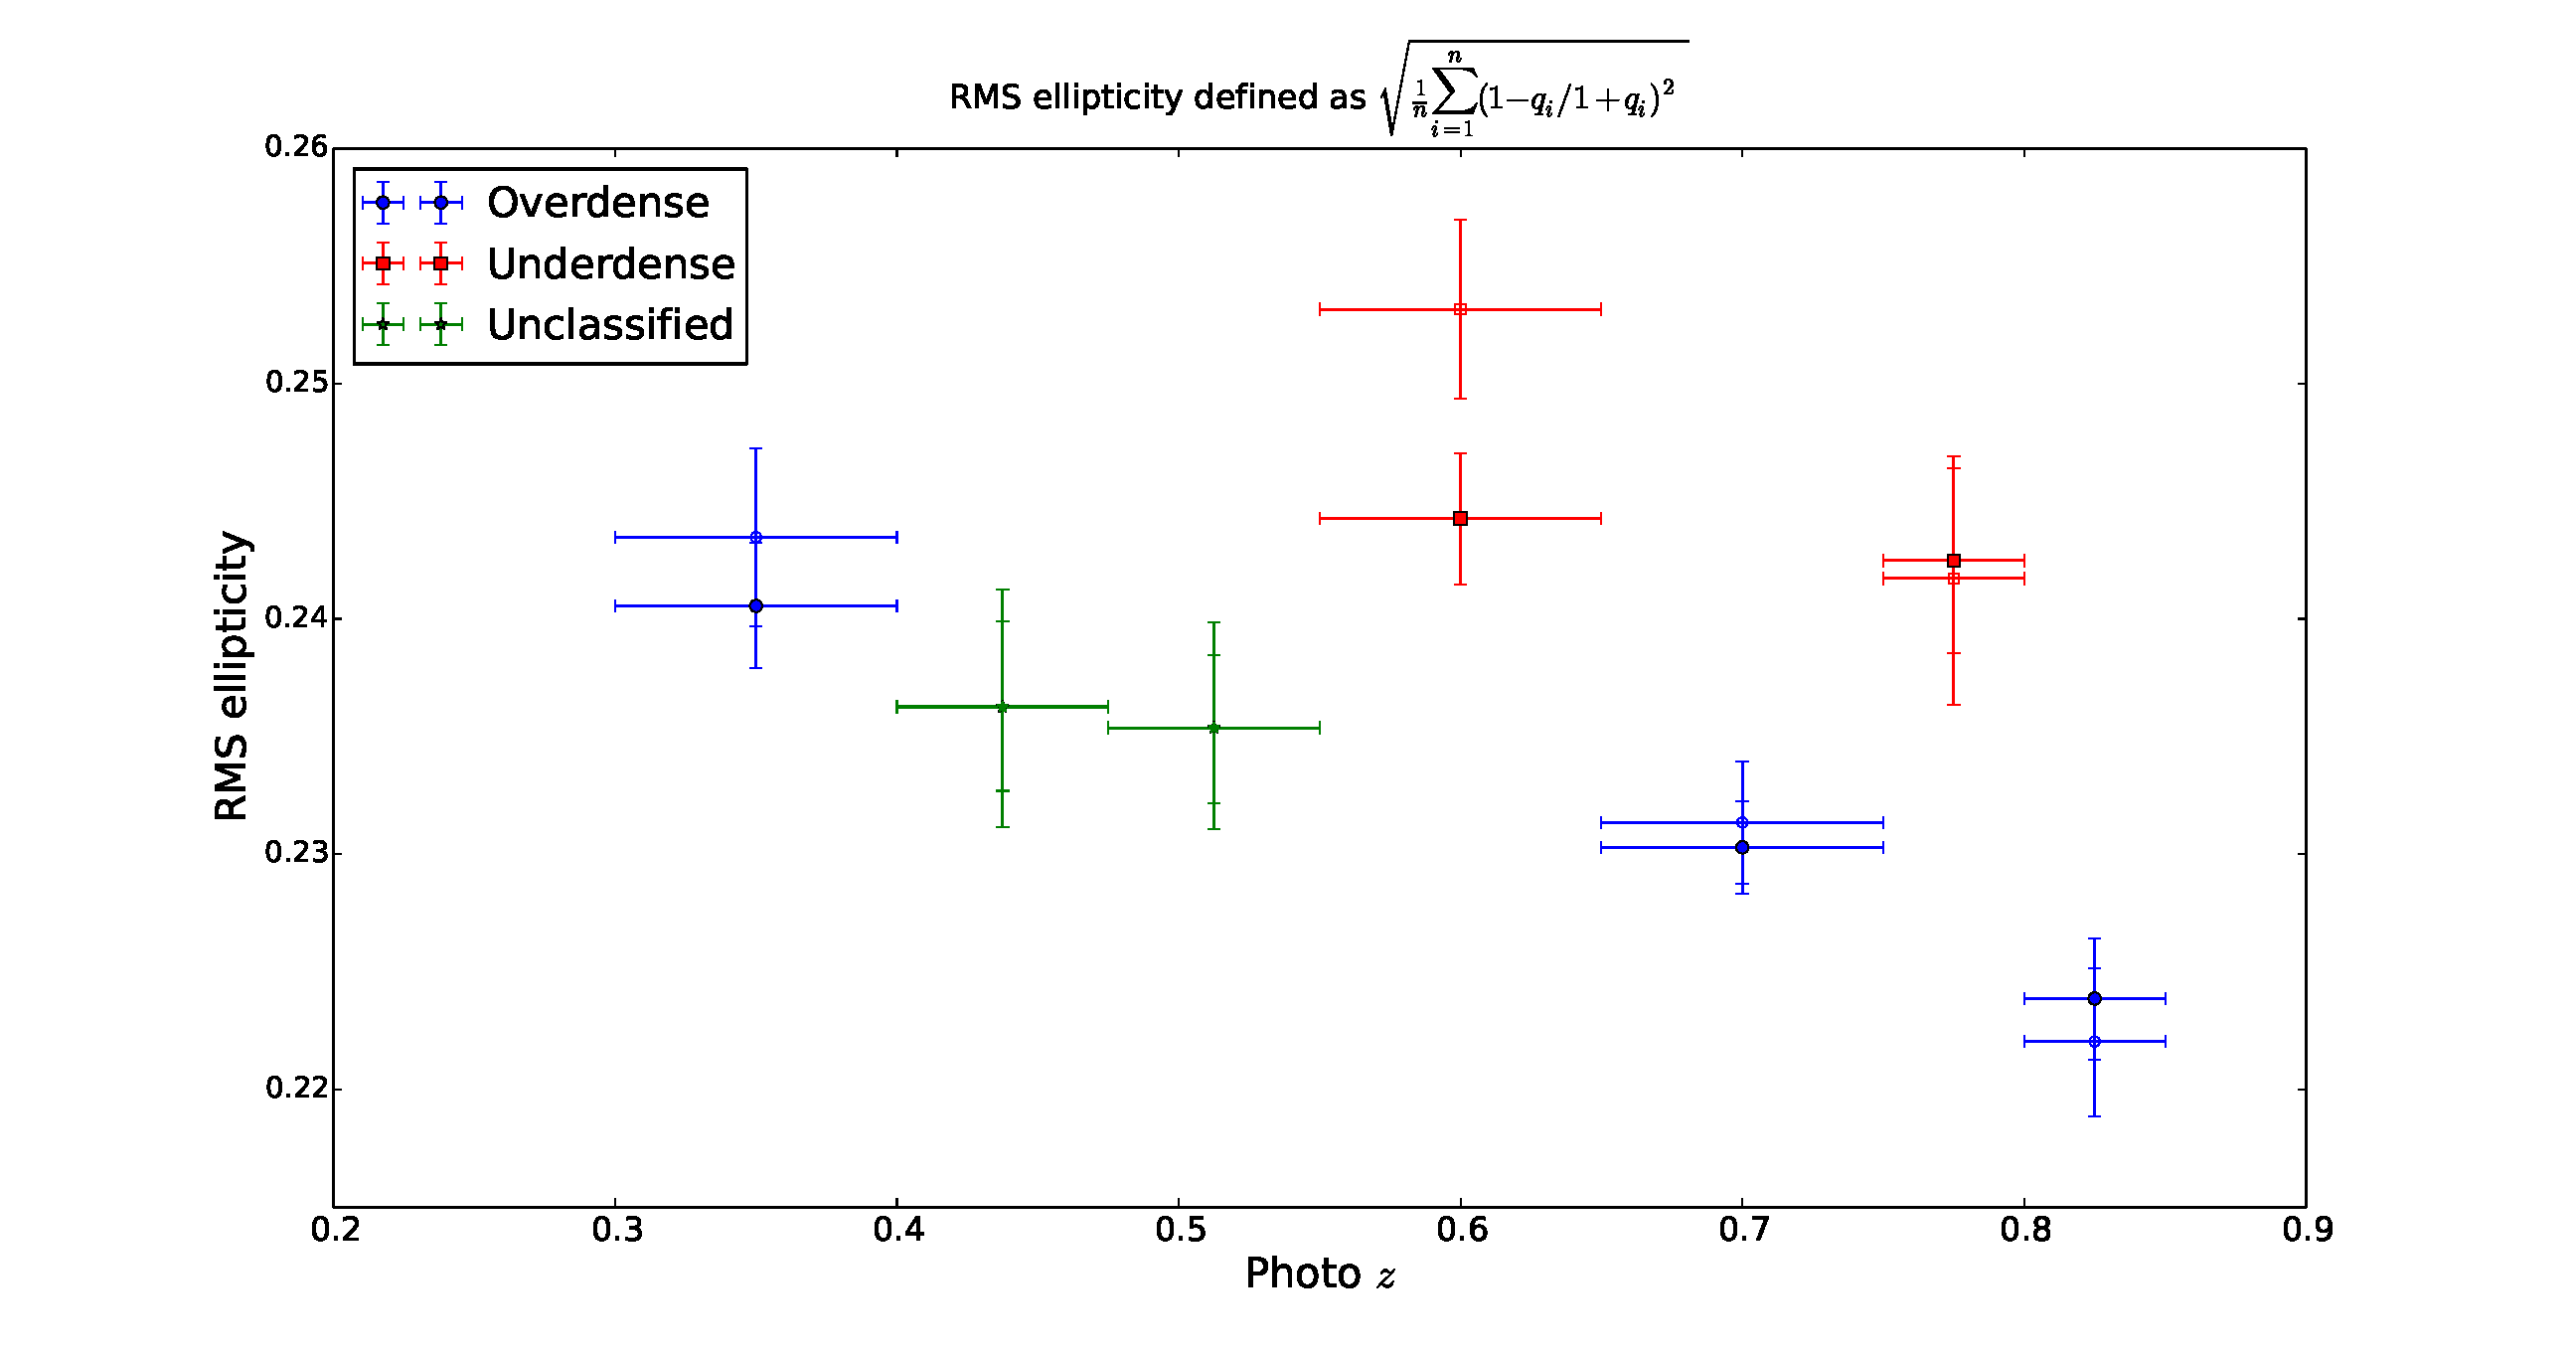
\includegraphics[width=0.9\columnwidth]{rms_ellip1_Bbandevolution_masscut.eps} \
 b) 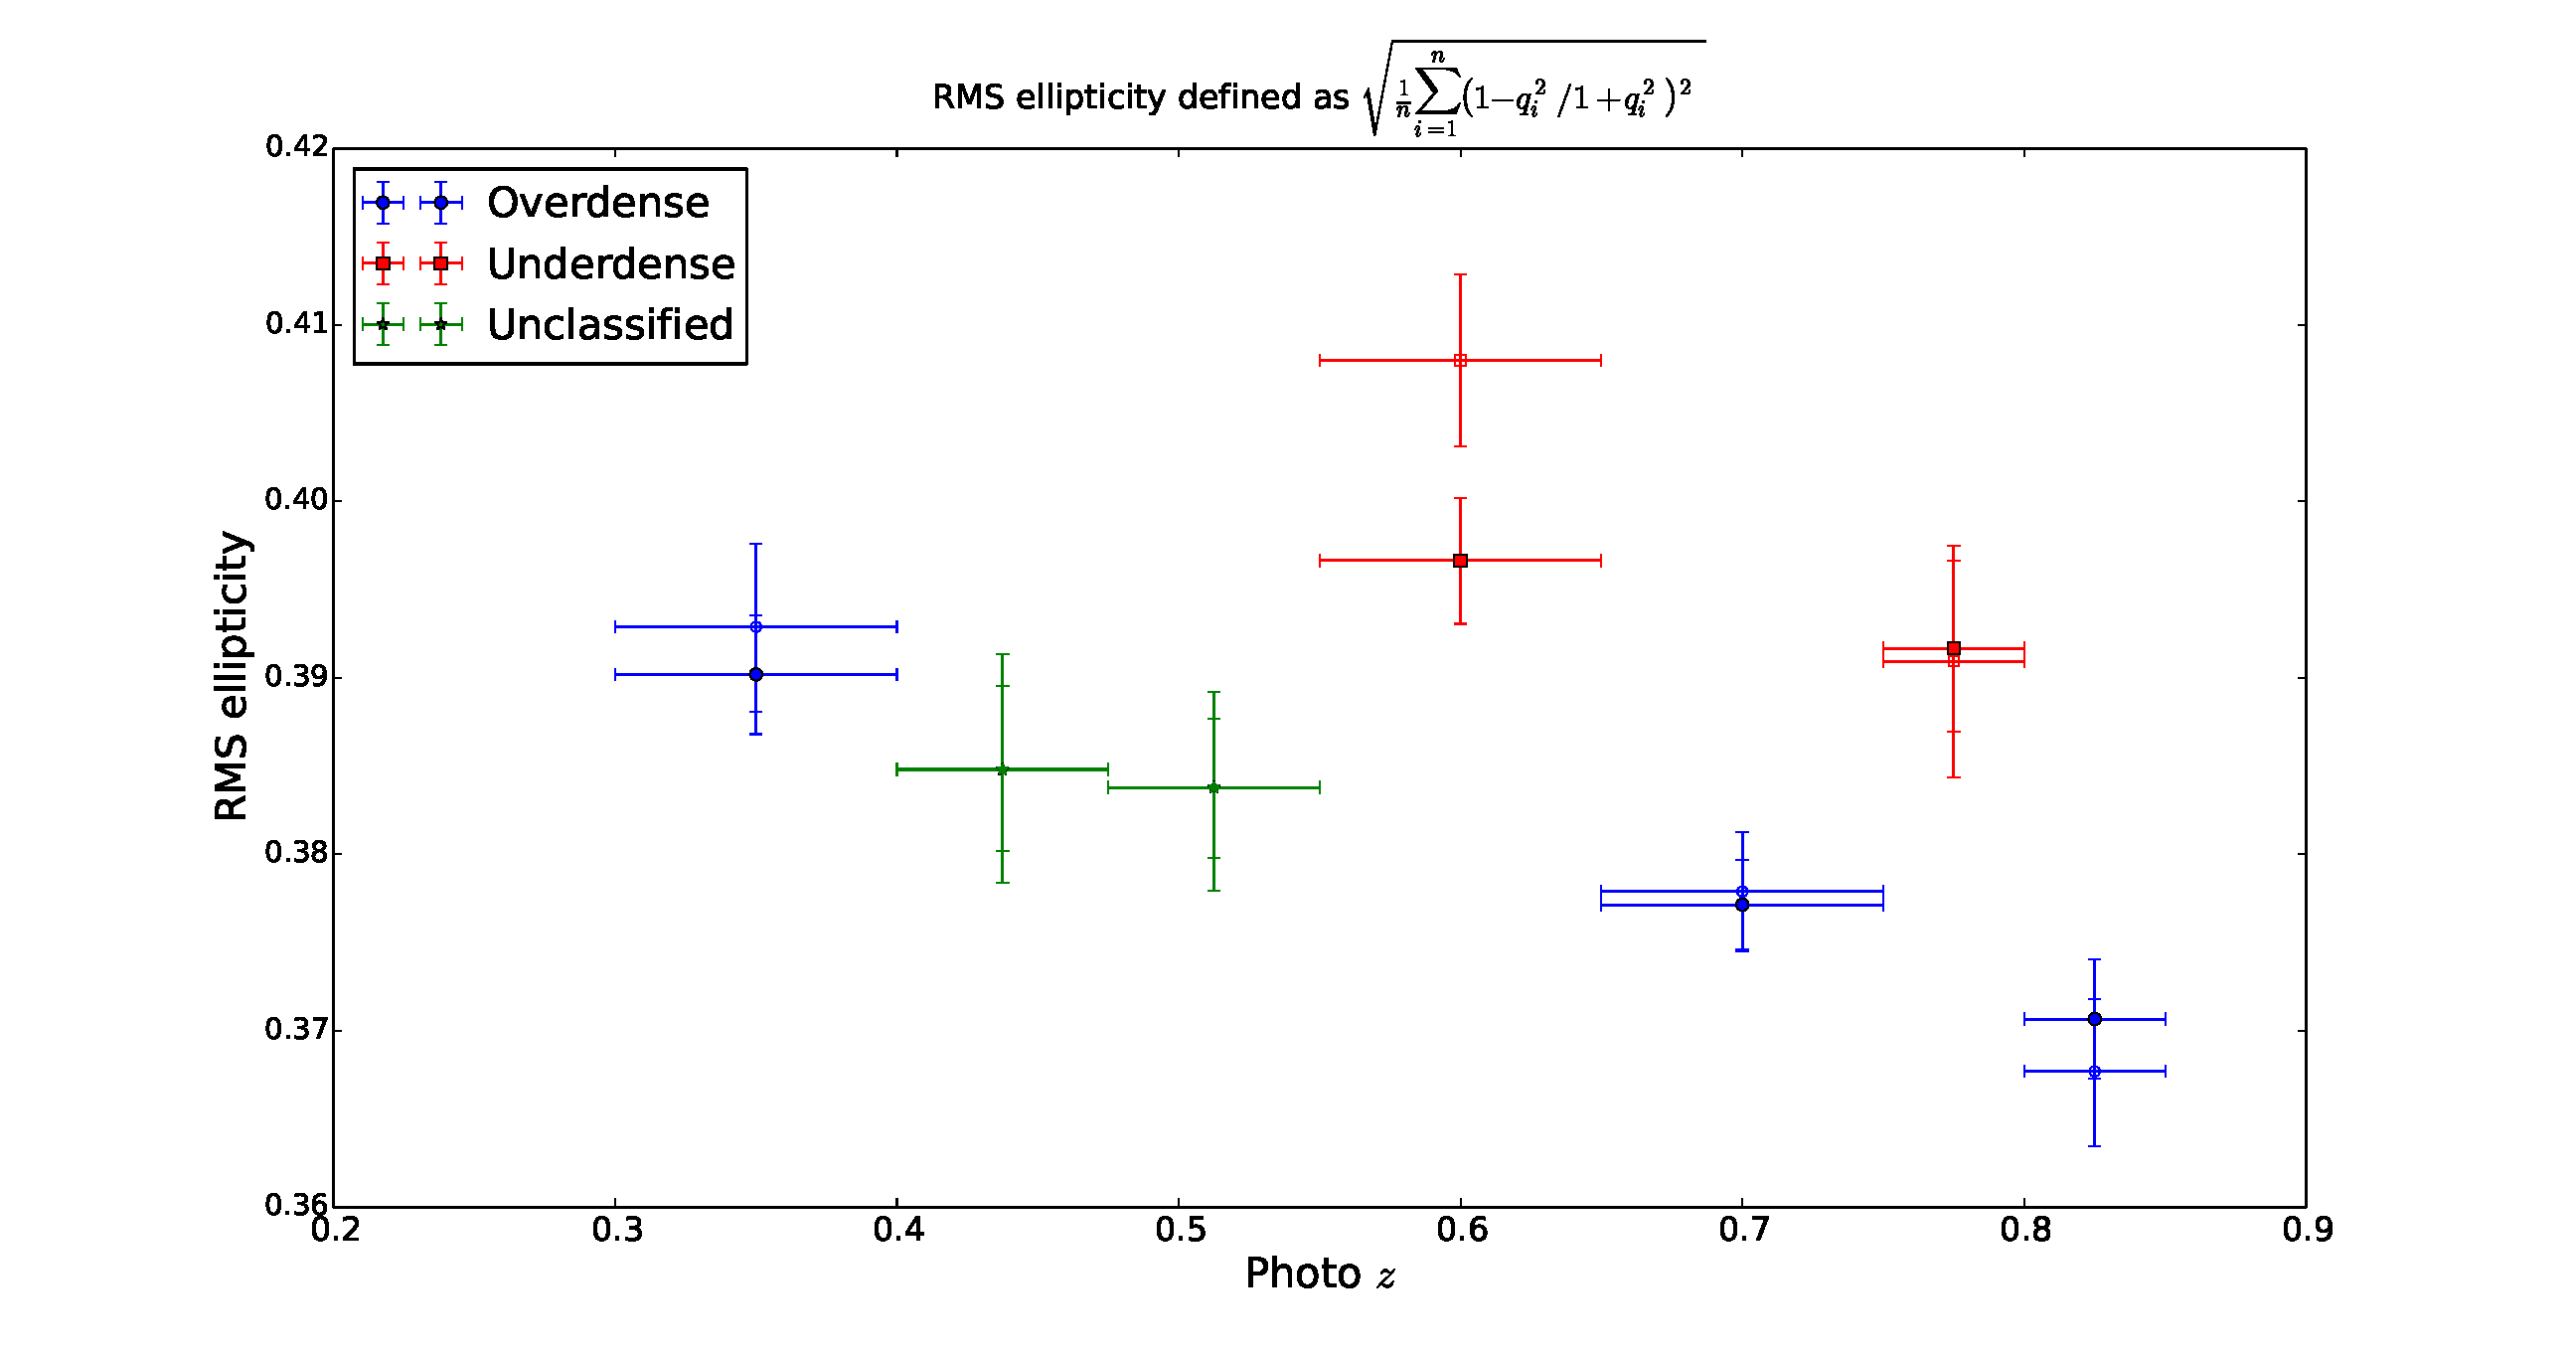
\includegraphics[width=0.9\columnwidth]{rms_ellip2_Bbandevolution_masscut.eps} \\
 \caption{Left: RMS ellipticities with ellipticity defined as $\frac{1-q}{1+q}$. \; 
          Right: RMS ellipticities with ellipticity defined as $\frac{1-q^2}{1+q^2}$.\\ The horizontal errorbars simply correspond to the binwidth while the vertical ones
          are $1\sigma$ errorbars obtained by bootstrapping. The solid points correspond to the sample where the luminosity cut evolves by -1.23 per unit redshift and the unfilled
          points correspond to the sample obtained from stellar mass cuts.}
 \label{fig:rms_ellip}
\end{figure*}

\end{document}


